\Opensolutionfile{ans}[ans/ans-2H3-TL-3]
\setcounter{dang}{0}
\setcounter{vd}{0}
\section{Ứng dụng của phương pháp tọa độ}
\subsection{Tóm tắt lý thuyết}
\begin{tomtat}
\underline{Phương pháp}
	\begin{itemize}
		\item \textbf{Bước} $1$: Chọn hệ trục tọa độ Oxyz trong không gian: Vì $Ox$, $Oy$, $Oz$ vuông góc với nhau từng đôi một nên nếu hình vẽ bài toán cho có chứa các cạnh vuông góc thì ta ưu tiên chọn các cạnh đó	làm trục tọa độ.
		\item \textbf{Bước} $2$: Suy ra tọa độ của các đỉnh, điểm trên hệ trục tọa độ vừa ghép.
		\item  \textbf{Bước} $3$: Sử dụng các kiến thức về tọa độ không gian để giải quyết bài toán
	\end{itemize}
\end{tomtat}
\subsection{Dạng toán và bài tập}
\begin{dang}{Các bài toán liên quan đến góc}
	\begin{itemize}
		\item Cho hai đường thẳng $d_1$, $d_2$ lần lượt có các VTPT là $\vec{u}_1,\vec{u}_2$.\\
		Góc giữa $d_1$ và $d_2$ bằng hoặc bù với góc giữa $\vec{u}_1$ và $\vec{u}_2$.\\
		Tức là $\cos (d_1,d_2 )=\left| \cos (\vec{u}_1,\vec{u}_2 ) \right|=\dfrac{\left| \vec{u}_1\cdot\vec{u}_2 \right|}{\left| \vec{u}_1 \right|\cdot\left| \vec{u}_2 \right|}$.
		\item Cho đường thẳng $d$ có VTCP $\vec{u}_d$ và mặt phẳng $(\alpha)$ có VTPT $\vec{n}_\alpha$.\\
		Góc giữa đường thẳng $d$ và mặt phẳng $(\alpha)$ bằng góc giữa đường thẳng $d$ với hình chiếu $d'$ của nó trên $(\alpha)$. Tức là $\sin (d,(\alpha ) )=\left| \cos (\vec{u}_d,\vec{n}_\alpha ) \right|=\dfrac{\left| \vec{u}_d\cdot\vec{n}_\alpha \right|}{\left| \vec{u}_d \right|\cdot\left| \vec{n}_\alpha \right|}$.
		\item Giả sử $(\alpha):Ax+By+Cz+D=0$ và $(\beta): A'x+B'y+C'z+D'=0$ có các véc-tơ pháp tuyến tương ứng là $\vec{n}_{\alpha}=(A;B;C)$ và $\vec{n}_{\beta}=(A';B';B')$. Khi đó, góc $\varphi$ giữa hai mặt phẳng $(\alpha)$ và $(\beta)$ được tính theo công thức
		$$\cos\varphi=\vert \cos(\vec{n}_{\alpha},\vec{n}_{\beta})\vert=\dfrac{\vert\vec{n}_{\alpha}\cdot\vec{n}_{\beta}\vert}{\vert\vec{n}_{\alpha}\vert\cdot\vert\vec{n}_{\beta}\vert}.$$
	\end{itemize}
\end{dang}
\noindent
\subsubsection{Ví dụ minh hoạ}
\begin{vd}%[Đề thi thử Toán 2018 THPT Quốc gia lần 1 trường Lý Thái Tổ]%[Lê Ngọc Hiếu-EX-7]%[2H3K4-1]
	Hình chóp $S.ABC$ có đáy là tam giác vuông tại $B$ có $AB=a$,  $AC =2a$. $SA$ vuông góc với mặt phẳng đáy, $SA = 2a$. Gọi $\psi$ là góc tạo bởi hai mặt phẳng $(SAC)$ và $(SBC)$. Tính $\cos\psi$.
	\choice
	{$\dfrac{\sqrt{3}}{2}$}
	{\True $\dfrac{\sqrt{15}}{5}$}
	{$\dfrac{\sqrt{3}}{5}$}
	{$\dfrac{1}{2}$}
	\loigiai{
		\immini{Chọn hệ trục tọa độ $Bxyz$ như hình vẽ.\\
			Ta tính được $B(0;0;0)$, $A(a;0;0)$, $C(0;a \sqrt{3};0)$, $S(a;0;2a)$,\\
			$\vv{SA}=(0;0;-2a)$, $\vv{SB}=(-a;0;-2a)$, $\vv{SC}=(-a;a\sqrt{3};-2a)$,\\
			$\vv{n_1}= \left[ \vv{SA} ; \vv{SC} \right] = (2a^2\sqrt{3};2a^2;0)$ là VTPT của $(SAC)$,\\
			$\vv{n_2}= \left[ \vv{SB} ; \vv{SC} \right] = (2a^2\sqrt{3};0;-a^2\sqrt{3})$ là VTPT của $(SBC)$.\\
			Ta có $$\cos \psi = \big|\cos \left[\vv{n_1};\vv{n_2}\right]\big|=\dfrac{|\vv{n_1}\vv{n_2}|}{|\vv{n_1}|\cdot |\vv{n_2}|}=\dfrac{\sqrt{15}}{5}.$$
		}{\begin{tikzpicture}[scale=.8]
			\tkzDefPoints{0/0/A, 2/-2/B, 7/0/C}
			\coordinate (S) at ($(A)+(0,5)$);
			\tkzDefPointBy[homothety = center B ratio 1.7](A)
			\tkzGetPoint{E}
			\tkzDefPointBy[homothety = center B ratio 1.4](C)
			\tkzGetPoint{F}
			\coordinate (G) at ($(B)+(0,7)$);
			\tkzDrawSegments[dashed](A,C)
			\tkzDrawSegments(S,A S,B B,C S,C A,B)
			\tkzLabelPoints[below left](A,B)
			\tkzLabelPoints[below right](C)
			\tkzLabelPoints[above](S)
			\tkzMarkRightAngle(A,B,C)
			\tkzDrawVectors(B,E B,F B,G)
			\draw (-1.5,1.5)[left]node{$x$} (9,0)node[above]{$y$} (2.5,5)node{$z$};
			\draw (0,2)node[above left]{$2a$};
			\draw (1.3,-1.5)node[above left]{$a$};
			\draw (3,0) node[above]{$2a$};
			\end{tikzpicture}
	}}
\end{vd}
\begin{vd}%[TT lần 1, Sở giáo dục Hà Nội, năm 2018]%[2H3K4-1]
	Cho hình chóp tứ giác đều $S.ABCD$ có tất cả các cạnh bằng nhau. Gọi $E$, $M$ lần lượt là trung điểm của các cạnh $BC$ và $SA$, $\alpha$ là góc tạo bởi đường thẳng $EM$ và mặt phẳng $(SBD)$. Tính $\tan\alpha$.
	\choice
	{$\sqrt 3$}
	{$2$}
	{\True $\sqrt 2$}
	{$1$}
	\loigiai{
		\immini{Không mất tính tổng quát, giả sử các cạnh của hình chóp bằng $2\sqrt2$.\\
			Chọn hệ trục tọa độ như hình vẽ.\\
			Khi đó: $E(1;1;0)$, $M(0;-1;1)$, $\vec{ME}=(1;2;-1)$ và $\vec{OC}=(0;2;0)$ là véc-tơ pháp tuyến của $(SBD)$.\\
			Do đó,\\ $\sin \alpha=\sin \left(EM,(SBD)\right)=\left|\cos \left(\vec{EM},\vec{OC}\right)\right|=\dfrac{\left|\vec{EM}\cdot\vec{OC}\right|}{\left|\vec{EM}\right|\cdot \left|\vec{OC}\right|}=\dfrac{2}{\sqrt6}.$\\
			Vậy $\tan\alpha =\dfrac{\sin\alpha}{\cos \alpha}=\dfrac{\sin \alpha}{\sqrt{1-\sin^2 \alpha}}=\sqrt 2$.
		}{\begin{tikzpicture}[scale=0.5]
			\tkzDefPoints{-2/1/A, 4/1/B,-4/-1/D, 0/6/S}
			\tkzDefLine[parallel=through B](A,D) \tkzGetPoint{h}
			\tkzDefLine[parallel=through D](A,B) \tkzGetPoint{k}
			\tkzInterLL(B,h)(D,k) \tkzGetPoint{C}
			\tkzDefMidPoint(A,C)\tkzGetPoint{O}
			\tkzDefMidPoint(B,C)\tkzGetPoint{E}
			\tkzDefMidPoint(A,S)\tkzGetPoint{M}
			\coordinate(x) at ($(O) !1.35! (B)$);
			\coordinate(y) at ($(O) !1.5! (C)$);
			\coordinate(z) at ($(O) !1.35! (S)$);
			\tkzDrawPoints(A,B,C,D,S,O,M,E)
			\tkzLabelPoints[below](A,B,C,D,O,M,E,x,y)
			\tkzLabelPoints[left](S,z)
			\tkzDrawSegments (S,B S,C S,D D,C C,B)
			\tkzDrawSegments[dashed](D,A A,B S,A A,C B,D S,O M,E)
			\tkzDrawSegments[->](B,x C,y S,z)
			\end{tikzpicture}}
	}
\end{vd}

\begin{vd}%[Thi thử L1, Cộng Hiền, Hải Phòng, 2018]%[Dương Xuân Lợi, 12EX11]%[2H3K4-1]
	\immini{Cho hình chóp $S.ABCD$ có đáy $ABCD$ là hình chữ nhật và cạnh bên $SA$ vuông góc với đáy. Biết rằng $AB=a$, $AD=a\sqrt{2}$, $SA=2a$. Gọi góc giữa hai mặt phẳng $(SBC)$ và mặt phẳng $(SBD)$ là $\alpha$. Tính $\cos\alpha$. (tham khảo hình vẽ bên)
		\choice
		{$\cos\alpha=\sqrt{\dfrac{1}{5}}$}
		{$\cos\alpha=\dfrac{3\sqrt{119}}{34}$}
		{\True $\cos\alpha=\sqrt{\dfrac{5}{7}}$}
		{$\cos\alpha=\sqrt{\dfrac{2}{3}}$}
	}{\begin{tikzpicture}[scale=0.9, font=\footnotesize, line join=round, line cap=round,>=stealth]
		\tkzDefPoints{0/0/A,-1.3/-1.6/B,2.5/-1.6/C}
		\coordinate (D) at ($(A)+(C)-(B)$);
		\coordinate (S) at ($(A)+(0,3)$);
		\tkzDrawPolygon(S,B,C,D)
		\tkzDrawSegments(S,C)
		\tkzDrawSegments[dashed](A,S A,B A,D B,D)
		\tkzDrawPoints[fill=black,size=4](D,C,A,B,S)
		\tkzLabelPoints[above](S)
		\tkzLabelPoints[below](A,B,C)
		\tkzLabelPoints[right](D)
		\end{tikzpicture}
	}
	\loigiai{
		\immini{
			Chọn hệ trục tọa độ như hình vẽ, ta có
			$A(0;0;0)$, $B(a;0;0)$, $D(0;a\sqrt{2};0)$, $C(a;a\sqrt{2};0)$, $S(0;0;2a)$.\\
			$\overrightarrow{BC}=(0;a\sqrt{2};0)$, $\overrightarrow{BS}=(-a;0;2a)$, $\overrightarrow{BD}=(-a;a\sqrt{2};0)$.\\
			$(SBC)$ có một véc-tơ pháp tuyến $\overrightarrow{n}_1=[\overrightarrow{BC},\overrightarrow{BS}]=(2a^2\sqrt{2};0;a^2\sqrt{2})$.\\
			$(SBD)$ có  một véc-tơ pháp tuyến $\overrightarrow{n}_2=[\overrightarrow{BS},\overrightarrow{BD}]=(-2a^2\sqrt{2};-2a^2;-a^2\sqrt{2})$.\\
			$\cos\alpha=\left|\cos\left(\overrightarrow{n}_1,\overrightarrow{n}_2\right)\right|=\dfrac{\left|\overrightarrow{n}_1\cdot\overrightarrow{n}_2\right|}{\left|\overrightarrow{n}_1\right|\cdot\left|\overrightarrow{n}_2\right|}=\sqrt{\dfrac{5}{7}}$.
		}{\begin{tikzpicture}[scale=0.8, font=\footnotesize, line join=round, line cap=round,>=stealth]
			\tkzDefPoints{0/0/A,-1.3/-1.6/B,2.5/-1.6/C}
			\coordinate (D) at ($(A)+(C)-(B)$);
			\coordinate (S) at ($(A)+(0,3)$);
			\coordinate (D1) at ($(A)!5/4!(D)$);
			\coordinate (B1) at ($(A)!1.4!(B)$);
			\coordinate (S1) at ($(A)!5/4!(S)$);
			\tkzDrawPolygon(S,B,C,D)
			\tkzDrawSegments(S,C)
			\tkzDrawSegments[dashed](A,S A,B A,D B,D)
			\draw[->] (B)--(B1) node[below]{$x$};
			\draw[->] (D)--(D1) node[below]{$y$};
			\draw[->] (S)--(S1) node[right]{$z$};
			\tkzDrawPoints[fill=black,size=4](D,C,A,B,S)
			\tkzLabelPoints[left](S)
			\tkzLabelPoints[below](A,B,C)
			\tkzLabelPoints[above right](D)
			\end{tikzpicture}
		}
	}
\end{vd}
\begin{vd}%[TT-Đặng Thúc Hứa- Nghệ An lần 2 - 2018]%[PhanMinhTâm, Ex10]%[2H3K4-1]
Cho hình chóp $ S.ABCD $ có đáy là hình chữ nhật, $ AB=3 $, $ BC=4 $. Tam giác $ SAC $ nằm trong mặt phẳng vuông góc với đáy, khoảng cách từ điểm $ C $ đến đường thẳng $ SA $ bằng $ 4 $. Cô-sin góc giữa hai mặt phẳng $ (SAB) $ và $ (SAC) $ bằng bao nhiêu?
		\choice
		{$ \dfrac{5\sqrt{34}}{17} $}
		{\True $ \dfrac{3\sqrt{34}}{34} $}
		{$ \dfrac{3\sqrt{17}}{17} $}
		{$ \dfrac{2\sqrt{34}}{17} $}
	\loigiai{
		\immini{
			Gọi $ K $ là hình chiếu của $ C $ lên $ SA $, ta có $ CK=4 $, $ AK=3 $, $ AC=5 $.\\
			Gọi $ H $ là hình chiếu của $ K $ lên $ (ABCD) $, ta có $ KH\perp(ABCD) $.\\
			Gọi $ I $ là trung điểm $ KB $. Ta có\\
			$ \heva{&KB\perp AI\\&KB\perp CI\\}\Rightarrow KB\perp AC $.\\
			$ \heva{&KH\perp AC\\&KB\perp AC\\}\Rightarrow AC\perp BH$.\\
			Ta có \begin{itemize}
				\item $ HK=\dfrac{KA\cdot KC}{AC}=\dfrac{12}{5} $,
				\item $ HA=\sqrt{9-\left( \dfrac{12}{5}\right)^2 }=\dfrac{9}{5} $,
				\item $ HB=\dfrac{AB\cdot BC}{AC}=\dfrac{12}{5} $.
			\end{itemize}
		}{
			\begin{tikzpicture}[thick,>=stealth,scale=0.6]
			\tkzDefPoints{4/9/S, 2/3/A, 6/0/C, 9/3/B, -1/0/D}
			\coordinate (O) at ($(A)!.5!(C)$);
			\coordinate (H) at ($(A)!.5!(O)$);
			\coordinate (K) at ($(A)!.5!(S)$);
			\coordinate (I) at ($(K)!.5!(B)$);
			\tkzDefPoint(8,-1.5){X}
			\tkzDefPoint(10,3.125){Y}
			\coordinate (Z') at ($(K)+(0,1.3)$);
			\coordinate (Z) at ($(K)+(0,3)$);
			\draw[->] (Z')--(Z)node[left]{$ z $};
			\draw[->] (C)--(X)node[above]{$ x $};
			\draw[->] (B)--(Y)node[right]{$ y $};
			\tkzDrawSegments(S,C C,B S,B S,D C,D)
			\tkzDrawSegments[dashed](A,B A,D S,A A,C K,H K,B A,I C,I C,K B,H K,Z')
			\tkzLabelPoints[right](K)
			\tkzLabelPoints[above left](A)
			\tkzLabelPoints[below left](D,H)
			\tkzLabelPoints[above](S,I)
			\tkzLabelPoints[below](C,B)
			\tkzDrawPoints[fill=black,size=1](A,B,C,S,D,H,K,I)
			\end{tikzpicture}
		}
		\noindent Chọn hệ trục tọa độ như hình vẽ, ta có $ H(0;0;0) $, $ B\left( 0;\dfrac{12}{5};0\right)  $, $ A\left( -\dfrac{9}{5};0;0 \right)  $, $ K\left( 0;0;\dfrac{12}{5} \right)  $.\\Ta có
		$ \vec{KA}=\left( -\dfrac{9}{5};0;-\dfrac{12}{5} \right)  $, $ \vec{KB}=\left( \dfrac{9}{5};\dfrac{12}{5};0 \right)  $.\\
		Véc-tơ pháp tuyến của mặt phẳng $ (SAB) $ là $ \vec{n}_1=\left( -16;12;12 \right) $.\\
		Véc-tơ pháp tuyến của mặt phẳng $ (SAC) $ là $ \vec{j}=(0;0;1) $.\\
		Do đó $ \cos((SAB),(SAC))=\dfrac{|12|}{\sqrt{0^2+0^2+1^2}\sqrt{16^2+12^2+12^2}}=\dfrac{3\sqrt{34}}{34}. $
	}
\end{vd}
\subsubsection{Bài tập rèn luyện}
\begin{ex}%[Đề THPT L1, Hoàng Mai, Nghệ An 2018]%[Thái Văn Đạt, EX10]%[2H3G4-1]
	Hình chóp $S.ABC$ có đáy $ABC$ là tam giác vuông tại $A$ với $AB=a$, $\widehat{ACB}=30^\circ$ và $SA=SB=SD$ với $D$ là trung điểm $BC$. Biết khoảng cách giữa hai đường thẳng $SA$ và $BC$ bằng $\dfrac{3a}{4}$. Tính $\cos$ góc giữa hai mặt phẳng $(SAC)$ và $(SBC)$.
	\choice
	{$\dfrac{2\sqrt{5}}{11}$}
	{\True $\dfrac{\sqrt{65}}{13}$}
	{$3$}
	{$\dfrac{\sqrt{5}}{33}$}
	\loigiai{
		\immini
		{
			Do tam giác $ABC$ vuông tại $A$ có $D$ là trung điểm $BC$ và $\widehat{ACB}=60^\circ$ nên tam giác $ABD$ đều cạnh $a$ và $BC=2a$, $CA=a\sqrt{3}$.\\
			Dựng $SH\perp(ABC)$ với $H\in(ABC)$.\\
			$\Rightarrow$ $H$ là tâm tam giác đều $BAD$ do $SA=SB=SD$.\\
			Gọi hình chiếu của $H$ lên $AB$, $AC$ thứ tự là $E$, $F$.\\
			Gọi $M$ là trung điểm đoạn $BD$.\\
			$\Rightarrow$ $AM=\sqrt{BA^2-BM^2}=\sqrt{a^2-\dfrac{a^2}{4}}=\dfrac{a\sqrt{3}}{2}$.\\
			$\Rightarrow$ $AH=\dfrac{2}{3}AM=\dfrac{a\sqrt{3}}{3}$ và $HE=HM=\dfrac{AM}{3}=\dfrac{a\sqrt{3}}{6}$.\\
			Ta có: $SH\perp BC$, $AM\perp BC$ nên $BC\perp (SAM)$.\\
			Kẻ $MN\perp SA$ ($N\in SA$) thì $MN$ là đường vuông góc chung của $SA$ và $BC$ hay $MN=\dfrac{3a}{4}$.\\
			$\Rightarrow$ $NA=\sqrt{MA^2-MN^2}=\dfrac{a\sqrt{3}}{4}$.\\
		}
		{
			\begin{tikzpicture}[>=stealth,scale=1,x=1cm,y=1cm]
			\tkzInit[ymin=-3,ymax=6.5,xmin=-0.5,xmax=6.5]
			\tkzClip
			\tkzSetUpPoint[color=black,fill=white,size=6]
			\draw[->] (0,0)node[above left]{$O$}--(0,6)node[left]{$z$};
			\draw[->] (0,0)--(2.5,5)node[right]{$x$};
			\draw[->] (0,0)--(6,-2.4)node[above]{$y$};
			\tkzDefPoints{0/0/A, 1/2/B, 3/0/D, 5/-2/C, 1.33/5.66/S}
			\tkzCentroid(A,B,D) \tkzGetPoint{H}
			\tkzDefMidPoint(B,D) \tkzGetPoint{M}
			\tkzDefPointBy[projection=onto A--S](M)\tkzGetPoint{N}
			\tkzDefPointBy[projection=onto A--B](H)\tkzGetPoint{E}
			\tkzDefPointBy[projection=onto A--C](H)\tkzGetPoint{F}
			\tkzDrawSegments(S,A A,C S,C)
			\tkzDrawSegments[  dashed](S,D S,B S,H H,E H,F A,B A,D B,D C,D M,N A,H H,M S,M)
			\tkzDrawPoints(A,B,C,H,M,N,E,F,D,S)
			\tkzLabelPoints[below](E,F,A,C,M,D)
			\tkzLabelPoints[below right](H)
			\tkzLabelPoints[left](S,B)
			\tkzLabelPoints[above left = 1.5mm and -1.7mm](N)
			\end{tikzpicture}
		}
		Trong tam giác $SAM$ có $MN$, $SH$ là hai đường cao nên $AH\cdot AM=AN\cdot AS$.\\
		$\Rightarrow$ $AS=\dfrac{AH\cdot AM}{AN}=\dfrac{2a\sqrt{3}}{3}$
		$\Rightarrow$ $SH=\sqrt{SA^2-AH^2}=a$.\\
		Chọn hệ trục tọa độ với gốc tại $A$ và các trục tọa độ như hình vẽ với tia $Ox$ trùng với tia $AB$, tia $Oy$ trùng với tia $AC$ và tia $Oz$ vuông góc với mặt phẳng $(ABC)$ và có hướng theo $\vec{HS}$. Các đơn vị trên các trục bằng nhau và bằng $a$.\\
		Khi đó: $A(0;0;0)$, $B(1;0;0)$, $C(0;\sqrt{3};0)$.\\
		Do $HF=AE=\dfrac{a}{2}$, $HE=HM=\dfrac{a\sqrt{3}}{6}$ và $SH=a$ nên $S\left(\dfrac{1}{2};\dfrac{\sqrt{3}}{6};1\right)$.\\
		Véc-tơ pháp tuyến của mặt phẳng $(SAC)$ là $$\vec{n_1}=[\vec{AC},\vec{AS}]=\left(\sqrt{3};0;\dfrac{-\sqrt{3}}{2}\right).$$
		Véc-tơ pháp tuyến của mặt phẳng $(SBC)$ là $$\vec{n_2}=[\vec{BC},\vec{SC}]=\left(-\sqrt{3};-1;\dfrac{-\sqrt{3}}{3}\right).$$
		Gọi $\alpha$ là góc giữa hai mặt phẳng $(SAC)$ và $(SBC)$, ta có: $$\cos \alpha=|\cos (\vec{n_1};\vec{n_2})|=\dfrac{|\vec{n_1}\cdot\vec{n_2}|}{|\vec{n_1}||\vec{n_2}|}=\dfrac{\sqrt{65}}{13}.$$
	}
\end{ex}
\begin{ex}%[Đề KSCL, Số 2 An Nhơn, Bình Định 2018]%[Nguyễn Thị Kiều Ngân, dự án 12EX-10]%[2H3B4-1]
	Cho hình lăng trụ tam giác $ABC.A'B'C'$ có đáy là tam giác đều cạnh bằng $2a$, $AA'=a\sqrt{2}$. Hình chiếu vuông góc của $A'$ lên mặt phẳng $(ABC)$ trùng với trung điểm của cạnh $BA$. Tính $\sin$ của góc tạo bởi hai mặt phẳng $(AB'C)$ và $(BA'C')$.
	\choice
	{$\dfrac{4\sqrt{31}}{31}$}
	{$\dfrac{2\sqrt{31}}{31}$}
	{\True $\dfrac{8\sqrt{3}}{\sqrt{217}}$}
	{$\dfrac{3\sqrt{31}}{31}$}
	\loigiai{
		\immini{
			$A'H=\sqrt{AA'^2-AH^2}=a$.\\
			Chọn hệ trục tọa độ như hình vẽ bên.\\
			Không mất tính tổng quát có thể giả sử $a=1$.\\
			Ta có $H(0;0;0)$, $B(1;0;0)$, $C(0;\sqrt{3};0)$, $A(-1;0;0)$, $A'(0;0;1)$, $B'(2;0;1)$, $C'(1;\sqrt{3};1)$.\\
			Gọi $\varphi$ là góc giữa hai mặt phẳng $(AB'C)$ và $(BA'C')$.
			\begin{itemize}
				\item $\vv{AB'}=(3;0;1)$, $\vv{AC}=(1;\sqrt{3};0)$\\
				$\Rightarrow \vv{n}_1 =\left[ \vv{AB'}, \vv{AC} \right] =(-\sqrt{3};1;3\sqrt{3})$.
				\item $\vv{A'B}=(1;0;-1)$, $\vv{A'C'}=(1;\sqrt{3};0)$\\
				$\Rightarrow \vv{n}_2 =\left[ \vv{A'B}, \vv{A'C'} \right] =(\sqrt{3};-1;\sqrt{3})$.
				\item $\cos \varphi =\left| \cos \left( \vv{n}_1, \vv{n}_2 \right) \right|
				=\dfrac{\left| {\vv{n}_1 \cdot \vv{n}_2} \right|}{\left| {\vv{n}_1} \right| \cdot \left| {\vv{n}_2} \right|}
				=\dfrac{5}{\sqrt{31} \cdot \sqrt{7}}.\\
				\Rightarrow \sin \varphi =\dfrac{8\sqrt{3}}{\sqrt{217}}$.
			\end{itemize}
		}{
			\begin{tikzpicture}[>=stealth, scale=1]
			\tkzDefPoints{0/0/A, 1.5/-1.5/B, 4/0/C}
			\tkzDefMidPoint(A,B)\tkzGetPoint{H}
			\coordinate (A') at ($(H)+(0,5)$);
			\tkzDefPointsBy[translation=from A to A'](B,C){B'}{C'}
			\tkzDefPointBy[homothety=center H ratio 2](B)\tkzGetPoint{x}
			\tkzDrawVector[>=stealth](B,x)
			\tkzDefPointBy[homothety=center H ratio 1.4](C)\tkzGetPoint{y}
			\tkzDrawVector[>=stealth](C,y)
			\tkzDefPointBy[homothety=center H ratio 1.2](A')\tkzGetPoint{z}
			\tkzDrawVector[>=stealth](A',z)
			\tkzDrawSegments(A,B B,C A,A' B,B' C,C' A',B' B',C' A',C' A',H A,B' B',C A',B B,C')
			\tkzDrawSegments[dashed](A,C H,C)
			\tkzDrawPoints[fill=black](A,B,C,A',B',C',H)
			\tkzLabelPoints[left](A,A',H,z)
			\tkzLabelPoints[right](C')
			\tkzLabelPoints[below](B,C)
			\tkzLabelPoints[above](B',y)
			\tkzLabelPoints[above right](x)
			\tkzMarkRightAngles(A',H,C A',H,B B,H,C)
			\end{tikzpicture}
		}
	}
\end{ex}
\begin{ex}%[Đề thi thử, THPT Quỳ Hợp 2, Nghệ An 2018]%[Hùng Nam Lý, dự án EX9]%[2H3K4-1]
	\immini
	{
		Cho hình chóp tứ giác đều $S.ABCD$ có tất cả các cạnh bằng $a.$
		Gọi $M$ là trung điểm của cạnh $BC,$  $\alpha$ là góc giữa đường thẳng $SD$ và mặt phẳng $(SAM).$ Tính giá trị $\sin\alpha.$
		\choice
		{\True $\dfrac{2\sqrt{22}}{11}$}
		{$\dfrac{\sqrt{22}}{11}$}
		{$\dfrac{\sqrt{12}}{11}$}
		{$\dfrac{\sqrt{21}}{11}$}
	}
	{
		\begin{tikzpicture}[scale=1]
		\tkzInit[xmin=-3,ymin=-3,xmax=3,ymax=4.5]\tkzClip
		\tkzDefPoints{0/0/O, -2.5/-1/B, 1/-1/C, 0/4/S}
		\tkzDefPointBy[symmetry = center O](C)
		\tkzGetPoint{A}
		\tkzDefPointBy[symmetry = center O](B)
		\tkzGetPoint{D}
		\coordinate (M) at ($(B)!0.5!(C)$);
		\tkzDrawSegments[dashed](A,D A,C D,B S,A S,O A,B A,M)
		\tkzDrawSegments(C,D B,C S,D S,B S,C S,M)
		\tkzMarkRightAngle[size=.2](B,O,A)
		\tkzMarkRightAngle[size=.2](S,O,C)
		\tkzLabelPoints[left](A)
		\tkzLabelPoints[above right](S)
		\tkzLabelPoints[below](C,B)
		\tkzLabelPoints[below](M)
		\tkzLabelPoints[right](D)
		\tkzLabelPoints[below](O)
		\tkzDrawPoints(A,B,C,D,O,S,M)
		\end{tikzpicture}
	}
	\loigiai{
		\immini
		{
			Gọi $O=AC\cap BD.$ Vì $S.ABCD$ là hình chóp đều nên $SO\perp (ABCD).$\\
			Mặt khác $ABCD$ là hình vuông cạnh $a$ nên\\
			$OA=OC=OB=OD=\dfrac{a\sqrt{2}}{2}.$\\
			Xét tam giác $SOA$ vuông tại $O$\\
			$\Rightarrow SO=\sqrt{SA^2-OA^2}=\sqrt{a^2-\dfrac{a^2}{2}}=\dfrac{a\sqrt{2}}{2}.$\\
			Chọn hệ trục tọa độ $Oxyz$ như hình vẽ.\\
			Khi đó, tọa độ các điểm là $B\left(\dfrac{a\sqrt{2}}{2};0;0\right)$, $C\left(0;\dfrac{a\sqrt{2}}{2};0\right)$,
			$S\left(0;0;\dfrac{a\sqrt{2}}{2}\right)$,  $A\left(0;-\dfrac{a\sqrt{2}}{2};0\right)$, $D\left(-\dfrac{a\sqrt{2}}{2};0;0\right)$ và $M\left(\dfrac{a\sqrt{2}}{4};\dfrac{a\sqrt{2}}{4};0\right).$
		}
		{
			\begin{tikzpicture}[scale=1]
			\tkzInit[xmin=-4,ymin=-4,xmax=4,ymax=5.5]\tkzClip
			\tkzDefPoints{0/0/O, -2.5/-1/B, 1/-1/C, 0/4/S}
			\tkzDefPointBy[symmetry = center O](C)
			\tkzGetPoint{A}
			\tkzDefPointBy[symmetry = center O](B)
			\tkzGetPoint{D}
			\coordinate (M) at ($(B)!0.5!(C)$);
			\tkzDefPointWith[linear,K=1.3](O,B)
			\tkzGetPoint{x}
			\tkzDrawVectors[](B,x)
			\tkzDefPointWith[linear,K=1.4](O,C)
			\tkzGetPoint{y}
			\tkzDrawVectors[](C,y)
			\tkzDefPointWith[linear,K=1.2](O,S)
			\tkzGetPoint{z}
			\tkzDrawVectors[](S,z)
			\tkzDrawSegments[dashed](A,D A,C D,B S,A S,O A,B A,M)
			\tkzDrawSegments(C,D B,C S,D S,B S,C S,M)
			\tkzMarkRightAngle[size=.2](B,O,A)
			\tkzMarkRightAngle[size=.2](S,O,C)
			\tkzLabelPoints[left](A,x)
			\tkzLabelPoints[above right](S)
			\tkzLabelPoints[below](C,O,B)
			\tkzLabelPoints[below](M)
			\tkzLabelPoints[right](D,z,y)
			\tkzDrawPoints(A,B,C,D,O,S,M)
			\end{tikzpicture}
		}
		\noindent Ta có $\vec{SD}=\left(-\dfrac{a\sqrt{2}}{2};0;-\dfrac{a\sqrt{2}}{2}\right)\Rightarrow \vec{u}=\left(1;0;1\right)$ là véc-tơ chỉ phương của $SD.$\\
		Mặt khác $\vec{SA}=\left(0;-\dfrac{a\sqrt{2}}{2};-\dfrac{a\sqrt{2}}{2}\right)$, $\vec{AM}=\left(\dfrac{a\sqrt{2}}{4};\dfrac{3a\sqrt{2}}{4};0\right)$
		$\Rightarrow \left[\vec{SA},\vec{AM}\right]=\left(\dfrac{3a^2}{4};-\dfrac{a^2}{4};\dfrac{a^2}{4}\right)$\\
		$\Rightarrow \vec{n}=(3;-1;1)$ là véc-tơ pháp tuyến của mặt phẳng $(SAM).$\\
		Khi đó $\sin\alpha=\left|\cos(\vec{u},\vec{n})\right|=\left|\dfrac{\vec{u}\cdot \vec{n}}{|\vec{u}|\cdot |\vec{n}|}\right|=\left|\dfrac{3+0+1}{\sqrt{2}\cdot \sqrt{11}}\right|=\dfrac{2\sqrt{22}}{11}.$
	}
\end{ex}
\begin{ex}%[THPT Số 2 An Nhơn - Bình Định - Lần 3]%[Thang Minh Do Vu - Dự án 12-EX11-18]%[2H3K4-1]
	\immini{
		Cho hình lập phương $ ABCD.A'B'C'D' $ có $ M $, $ N $, $ E $, $ F $ lần lượt là trung điểm của cạnh $ A'B' $, $ A'D' $, $ B'C' $, $ C'D' $(tham khảo hình bên).
		Tính cosin của góc tạo giữa hai mặt phẳng $ (CMN) $ và $ (AEF) $.
		\choicew{0.4\textwidth}
		\choice
		{\True $ \dfrac{1}{17} $}
		{$ \dfrac{1}{2} $}
		{$ 0 $}
		{$ \dfrac{2}{17} $}
	}{
		\begin{tikzpicture}[scale=0.6, line join=round, line cap=round,>=stealth]
		\tkzDefPoints{0/0/A}
		\coordinate (B) at ($(A) + (-2,-1.5)$) ;
		\coordinate (D) at ($(A) + (5,0)$) ;
		\coordinate (C) at ($(D) + (-2,-1.5)$) ;
		\coordinate (C') at ($(C) + (0,5)$) ;
		\coordinate (A') at ($(A) + (0,5)$) ;
		\coordinate (B') at ($(B) + (0,5)$) ;
		\coordinate (D') at ($(D) + (0,5)$) ;
		\tkzDefMidPoint(A',B') \tkzGetPoint {M}
		\tkzDefMidPoint(A',D') \tkzGetPoint {N}
		\tkzDefMidPoint(B',C') \tkzGetPoint {E}
		\tkzDefMidPoint(C',D') \tkzGetPoint {F}
		\tkzDrawSegments(D,C D,D' B,C B,B' C,C' A',B' B',C' C',D' D',A' M,N E,F)
		\tkzDrawSegments[dashed](D,A A,B A,A' C,M C,N A,E A,F)
		\tkzLabelPoints(A,B,C,D,B',C',D',N,E,F)
		\tkzLabelPoints[above left](M)
		\tkzLabelPoints[above](A')
		\tkzDrawPoints[fill=black](A,B,C,D,A',B',C',D',M,N,E,F)
		\end{tikzpicture}
	}
	\loigiai{
		Cho độ dài của cạnh hình lập phương là $ 1 $. Đắt hệ trục tọa độ vuông góc $ Oxyz $ sao cho gốc $ O $ trùng với điểm $ A $, $ AB $ trùng với $ Ox $, $ AD $ trùng với $ Oy $ và $ AA' $ trùng với $ Oz $. Khi đó ta tính được tọa độ các điểm $ A(0,0,0) $, $ E\left (1;\dfrac{1}{2};1\right ) $, $ F\left (\dfrac{1}{2};1;1\right ) $, $ C(1;1;0) $, $ M\left (\dfrac{1}{2};0;1\right ) $, $ N\left (0;\dfrac{1}{2};1\right ) $.\\
		Ta tính được $ \overrightarrow{AE}= \left (1;\dfrac{1}{2};1\right )$, $ \overrightarrow{AF}=\left (\dfrac{1}{2};1;1\right ) $, $ \overrightarrow{CM}=\left (-\dfrac{1}{2};-1;1\right ) $, $ \overrightarrow{CN}=\left (-1;-\dfrac{1}{2};1\right ) $.\\
		$ \overrightarrow{n}_{(AEF)}=\left [\overrightarrow{AE};\overrightarrow{AF}\right ]=\left (-\dfrac{1}{2};-\dfrac{1}{2};\dfrac{3}{4}\right ). $\\
		$ \overrightarrow{n}_{(CMN)}=\left [\overrightarrow{CM};\overrightarrow{CN}\right ]=\left (-\dfrac{1}{2};-\dfrac{1}{2};-\dfrac{3}{4}\right ). $\\
		$ \cos \left [\overrightarrow{n}_{(AEF)}; \overrightarrow{n}_{(CMN)}\right ]=\dfrac{\overrightarrow{n}_{(AEF)}\cdot \overrightarrow{n}_{(CMN}}{\left |\overrightarrow{n}_{(AEF)}\right |\cdot \left |\overrightarrow{n}_{(CMN)}\right |} =-\dfrac{1}{17}$.\\
		Vậy cosin của góc tạo giữa hai mặt phẳng $ (CMN) $ và $ (AEF) $ là $ \dfrac{1}{17} $.
	}
\end{ex}

\begin{dang}{Các bài toán tính khoảng cách}
	\begin{itemize}
		\item Khoảng cách từ điểm $M(x_0;y_0;z_0)$ đến mặt phẳng $(P)$ có phương trình $Ax+By+Cz+D=0$ là $$d(M,(P))=\dfrac{|Ax_0+By_0+Cz_0+D|}{\sqrt{A^2+B^2+C^2}}.$$
		\item Cho đường thẳng $\Delta $ đi qua $M_0$, có VTCP $\vec{u}$ và điểm $M\notin \Delta $. Khi đó để tính khoảng cách từ $M$ đến $\Delta $ ta có công thức $\mathrm{d}\left[M,\Delta \right]=\dfrac{\left|\left[\vec{MM_0},\vec{u}\right] \right|}{\left| \vec{u} \right|}$.
		\item Cho hai đường thẳng chéo nhau $\Delta $ đi qua $M_0$ có VTCP $\vec{u}$ và $\Delta'$ đi qua $M_0'$ có VTCP $\vec{u'}$. Khi đó khoảng cách giữa hai đường thẳng $\Delta $ và $\Delta '$ được tính theo công thức $d(\Delta ,\Delta ' )=\dfrac{\left| \left[ \vec{u},\vec{u'} \right]\cdot\vec{M_0M'_0}\right|}{\left| \left[ \vec{u},\vec{u'} \right] \right|}$.
	\end{itemize}
\end{dang}
\subsubsection{Ví dụ minh hoạ}
\begin{vd}%[Phan Minh Tâm, dự án EX11-2018]%[2-BGD-102 - Đề thi chính thức THPT QG môn Toán mã 102 năm 2018]%[2H3K4-1]
	Cho hình chóp $S.ABCD$ có đáy là hình chữ nhật, $AB = a$, $BC = 2a$, $SA$ vuông góc với mặt phẳng đáy và $SA = a$. Khoảng cách giữa hai đường thẳng $BD$ và $SC$ bằng
	\choice
	{$\dfrac{4\sqrt{21}a}{21}$}
	{$\dfrac{\sqrt{30}a}{6}$}
	{$\dfrac{\sqrt{30}a}{12}$}
	{\True $\dfrac{2\sqrt{21}a}{21}$}
	\loigiai{
		\immini{
			Chọn hệ trục tọa độ như hình vẽ, ta có $ A(0;0;0) $, $ B(0;a;0) $, $ D(2a;0;0) $, $ C(2a;a;0) $ và $ S(0;0;a) $.\\
			Ta có
			\begin{itemize}
				\item $ \vec{BD}=(2a;-a;0) $.
				\item $ \vec{SC}=(2a;a;-a) $.
				\item $ \vec{SB}=(0;a;-a) $.
				\item $ [\vec{BD},\vec{SC}]=(a^2;2a^2;4a^2)\\ \Rightarrow \left|[\vec{BD},\vec{SC}] \right|=a^2\sqrt{21} $.
				\item $ \left| [\vec{BD},\vec{SC}]\cdot\vec{SB}\right|=2a^3 $.
			\end{itemize}
			Khoảng cách giữa hai đường thẳng $ BD $ và $ SC $ là $$ \mathrm{d}(SC,BD)=\dfrac{\left| [\vec{BD},\vec{SC}]\cdot\vec{SB}\right| }{\left| [\vec{BD},\vec{SC}] \right| }=\dfrac{2a\sqrt{21}}{21}. $$
		}{
			\begin{tikzpicture}[scale=.8,font=\footnotesize,line join= round,line cap=round,>=stealth,x=0.75cm,y=0.75cm]
			\tkzDefPoints{2/9/S, 2/3/A, 7/0/C, 9/3/B, 0/0/D, -0.67/-1/X, 10/3/Y, 2/10/Z}
			\tkzDrawSegments(S,C C,B S,B S,D C,D)
			\tkzDrawSegments[dashed](A,B A,D S,A B,D)
			\tkzLabelPoints[above](B)
			\tkzLabelPoints[above left](A)
			\tkzLabelPoints[left](D)
			\tkzLabelPoints[left](S)
			\tkzLabelPoints[below](C)
			\tkzDrawPoints(A,B,C,S,D)
			\draw[->] (D)--(X) node[left]{$x$};
			\draw[->] (B)--(Y)node[below left]{$y$};
			\draw[->] (S)--(Z)node[left]{$z$};
			\tkzMarkRightAngle(S,A,D)
			\tkzMarkRightAngle(S,A,B)
			\tkzMarkRightAngle(D,A,B)
			\end{tikzpicture}
		}
	}
\end{vd}
\begin{vd}%[2-TT-33-BenTre-VinhPhuc-18]%[Đoàn Nhật Thiện-12EX-8]%[2H3K4-1]
	Cho hình lăng trụ đứng $ABCD.A_1B_1C_1D_1$, đáy $ABCD$ là hình chữ nhật có $AB=a$, $AD=a\sqrt{3}$. Biết góc giữa đường thẳng $A_1C$ và mặt phẳng $(ABCD)$ bằng $60^\circ$. Tính khoảng cách giữa đường thẳng $B_1C$ và $C_1D$ theo $a$.
	\choice
	{$\dfrac{4a\sqrt{51}}{17} $}
	{$\dfrac{a\sqrt{51}}{17} $}
	{$\dfrac{8a\sqrt{51}}{17} $}
	{\True $\dfrac{2a\sqrt{51}}{17} $}
	\loigiai{
		\immini{Ta có $C_1D\parallel B_1A\Rightarrow C_1D\parallel (AB_1C)$\\
			$\Rightarrow \mathrm{d}(C_1D,B_1C)=\mathrm{d}(C_1D,(B_1AC))=\mathrm{d}(C_1,(AB_1C))$. $AA_1\perp (ABCD)$ suy ra $AC$ là hình chiếu của $A_1C$ lên mặt phẳng $(ABCD)$. Do đó góc tạo bởi $A_1C$ và mặt phẳng $(ABCD)$ là góc $\widehat{A_1CA}$.\\
			Ta có $AC=\sqrt{AB^2+BC^2}=\sqrt{AD^2+AB^2}=\sqrt{(a\sqrt{3})^2+a^2}=2a$.\\
			Xét tam giác $AA_1C$ có $$AA_1=AC\cdot \tan 60^\circ=2\sqrt{3}a.$$
			Chọn hệ trục với $A(0;0;0)$, $B(a;0;0)$, $D(0;a\sqrt{3};0)$, $C(a;a\sqrt{3};0)$, $A_1(0;0;2a\sqrt{3})$, $D_1(0;a\sqrt{3};2a\sqrt{3})$, $B_1(a;0;2a\sqrt{3})$; $C_1(a;a\sqrt{3};2a\sqrt{3})$. }{\begin{tikzpicture}[scale=0.5,>=stealth]
			\tkzDefPoints{0/0/A,-3/-3/B,7/0/D}
			\coordinate (C) at ($(B)+(D)-(A)$);
			\coordinate (A_1) at ($(A)+(0,7)$);
			\coordinate (B_1) at ($(A_1)+(B)-(A)$);
			\coordinate (C_1) at ($(A_1)+(C)-(A)$);
			\coordinate (D_1) at ($(A_1)+(D)-(A)$);
			\tkzMarkAngle(A_1,C,A)
			\tkzDrawPoints(A,B,C,D,A_1,B_1,C_1,D_1)
			\tkzDrawSegments(B,C C,D B,B_1 C,C_1 D,D_1 A_1,B_1 B_1,C_1 D_1,C_1 A_1,D_1 B_1,C C_1,D)
			\tkzDrawSegments[dashed](A,A_1 A,B A,D A_1,C A,C)
			\tkzLabelPoints[above](A_1,C_1,D_1)\tkzLabelPoints[below right](C,D)\tkzLabelPoints[below left](B_1,B)\tkzLabelPoints[below](A)
			\end{tikzpicture}}
		Ta có $\vec{AB_1}=(a;0;2a\sqrt{3})$, $\vec{AC}=(a;a\sqrt{3};0)$, $[\vec{AB_1},\vec{AC}]=\left(-6a^2;2\sqrt{3}a^2;\sqrt{3}a^2\right)$. Mặt phẳng $(AB_1C)$ qua ba điểm $A$, $B_1$, $C$.\\ Khi đó mặt phẳng $(AB_1C)$ có một véc-tơ pháp tuyến $\vec{n}=(-6,2\sqrt{3};\sqrt{3})$. Phương trình mặt phẳng $(AB_1C)\colon -6x+2\sqrt{3}y+\sqrt{3}z=0$.\\
		Khoảng cách từ $C_1$ đến $(AB_1C)$ là $$\mathrm{d}(C_1,(AB_1C))=\dfrac{|-6 \cdot a+2\sqrt{3} \cdot a\sqrt{3}+\sqrt{3}\cdot 2a\sqrt{3}|}{\sqrt{(-6)^2+(2\sqrt{3})^2+(\sqrt{3})^2}}=\dfrac{2a\sqrt{51}}{17}.$$
	}
\end{vd}
\begin{vd}%[Đề HK2, 2018, Sở Đồng Nai]%[Trần Quang Thạnh, dự án EX9]%[2H3K4-1]
	Cho hình chóp $S.MNPQ$ có đáy là hình vuông cạnh bằng $1$, $SM$ vuông góc với đáy và $SM=2$. Tính khoảng cách $h$ giữa hai đường thẳng $SN$ và $MP$.
	\choice
	{$h=\dfrac{1}{3} $}
	{$h=1 $}
	{$h=2 $}
	{\True $h=\dfrac{2}{3} $}
	\loigiai{
		\immini{Chọn hệ trục tọa độ $Oxyz$ sao cho $M(0;0;0)$, $S(0;0;2)$, $N(1;0;0)$, $Q(0;1;0)$. Lúc đó $P(1;1;0)$, $\vec{SN}=(1;0;-2)$, $\vec{MP}=(1;1;0)$ và $\vec{MN}=(1;0;0)$.\\
			Suy ra $\left[\vec{SN},\vec{MP}\right]=(2;-2;1)$, do đó
			$$h=\dfrac{\left|\left[\vec{SN},\vec{MP}\right]\cdot \vec{MN}\right|}{\left|\left[\vec{SN},\vec{MP}\right]\right|}=\dfrac{2}{3}.$$
		}{\begin{tikzpicture}[scale=0.7]
			\tkzDefPoints{0/0/N, 8/0/P, 10/2/Q, 2/2/M, 2/6/S}
			\tkzDrawPoints(S,M,N,P,Q)
			\tkzDrawSegments(N,P P,Q S,N S,P S,Q)
			\tkzDrawSegments[dashed](M,N M,Q S,M M,P)
			\tkzLabelPoints[above right](S,M,Q)
			\tkzLabelPoints[below right](N,P)
			\tkzMarkRightAngle(S,M,Q)
			\end{tikzpicture}}
	}
\end{vd}
\begin{vd}%[Đề TT, SGD, Đồng Tháp 2018]%[Phan Quốc Trí, dự án Ex10]%[2H3B4-1]
	Cho hình lập phương $ABCD.A'B'C'D'$ có cạnh là $a>0$. Khi đó khoảng cách giữa hai đường thẳng chéo nhau $AB'$ và $BC'$ là
	\choice
	{\True $\dfrac{a\sqrt{3}}{3}$}
	{$\dfrac{a\sqrt{6}}{3}$}
	{$\dfrac{a\sqrt{2}}{3}$}
	{$\dfrac{a\sqrt{3}}{2}$}
	\loigiai{
		\immini{
			Chọn hệ trục tọa độ $Oxyz$ sao cho $A$ trùng với gốc tọa độ và $B$, $D$, $A'$ lần lượt thuộc tia $Ox$, $Oy$, $Oz$.\\
			Ta có $A(0;0;0)$, $B'(a;0;a)$, $B(a;0;0)$, $C'(a;a;a)$.\\
			$\overrightarrow{AB'}=(a;0;a)$, $\overrightarrow{BC'}=(0;a;a)$ và $\overrightarrow{AB}=(a;0;0)$.\\
			$$\mathrm{d}(AB',BC')=\dfrac{\left| \left[\overrightarrow{AB'},\overrightarrow{BC'}\right] \cdot \overrightarrow{AB} \right|}{\left|\left[\overrightarrow{AB'},\overrightarrow{BC'}\right] \right|}=\dfrac{a\sqrt{3}}{3}.$$
		}{
			\begin{tikzpicture}[scale=0.8,>=stealth]
			\tkzDefPoints{0/0/A, 4/0/C, -1/-1.5/B, 0/3/E}
			%\tkzDefMidPoint(B,C) \tkzGetPoint{M}
			\tkzDefPointBy[translation=from A to B](C)\tkzGetPoint{D}
			\tkzDefPointBy[translation=from A to E](B)\tkzGetPoint{B'}
			\tkzDefPointBy[translation=from A to E](C)\tkzGetPoint{C'}
			\tkzDefPointBy[translation=from A to E](D)\tkzGetPoint{D'}
			\tkzDefPointBy[translation=from A to E](A)\tkzGetPoint{A'}
			\tkzDefPointBy[homothety=center A ratio 1.5](B) \tkzGetPoint{x}
			\tkzDefPointBy[homothety=center A ratio 1.4](C) \tkzGetPoint{y}
			\tkzDefPointBy[homothety=center A ratio 1.5](A') \tkzGetPoint{z}
			\tkzDrawSegments(B,D D,C D',C' D',B' B',A' A',C' B,B' D,D' C,C')
			\tkzDrawSegments[dashed](A,B A,C A,A' A,B' B,C')
			\tkzDrawSegments[->](B,x C,y A',z)
			\tkzLabelPoints(C,D,C',D')
			\tkzLabelPoints[left](A',B,B',A)
			\tkzLabelPoints(x,y,z)
			\tkzDrawPoints[fill=black](A,B,C,D,A',B',C',D')
			\end{tikzpicture}
		}
	}
\end{vd}
\subsubsection{Bài tập rèn luyện}
%chỗ này 10 câu ex tự luận
\begin{ex}%[TT-Đặng Thúc Hứa- Nghệ An lần 2 - 2018]%[PhanMinhTâm, Ex10]%[2H3K4-1]
	\immini{Cho hình chóp $ S.ABCD $ có đáy $ ABCD $ là hình chữ nhật, $ AB=2a $, $ BC=a $, tam giác $ SAB $ là tam giác đều và nằm trong mặt phẳng vuông góc với đáy. Gọi $ E $ là trung điểm của $ CD $. Tính theo $ a $ khoảng cách giữa hai đường thẳng $ BE $ và $ SC $.
		\choice
		{$ a $}
		{$ \dfrac{a\sqrt{15}}{5} $}
		{$ \dfrac{a\sqrt{3}}{2} $}
		{\True $ \dfrac{a\sqrt{30}}{10} $}
	}{
		\begin{tikzpicture}[thick,>=stealth,scale=0.4,every node/.style={scale=0.8}]
		\tkzDefPoints{1/9/S, 2/3/B, 7/0/D, 9/3/C, 0/0/A}
		\coordinate (H) at ($(A)!.5!(B)$);
		\coordinate (E) at ($(C)!.5!(D)$);
		\tkzDrawSegments(S,A A,D D,S D,C C,S)
		\tkzDrawSegments[dashed](A,B B,S B,C B,E)
		\tkzLabelPoints[left](B)
		\tkzLabelPoints[below](A)
		\tkzLabelPoints[below](D)
		\tkzLabelPoints[above](S)
		\tkzLabelPoints[right](C,E)
		\tkzDrawPoints[fill=black,size=1](A,B,C,S,D,E)
		\end{tikzpicture}
	}
	\loigiai{
		\immini{
			Chọn hệ trục tọa độ như hình vẽ, ta có $ H(0;0;0) $, $ B(-a;0;0) $, $ C(-a;a;0) $, $ E(0;a;0) $ và $ S(0;0;a\sqrt{3}) $.\\
			Ta có $ \vec{BE}=(a;a;0) $, $ \vec{SC}=(-a;a;-a\sqrt{3}) $, $ \vec{EC}=(-a;0;0) $.\\
			Khi đó, $ [\vec{BE},\vec{SC}] = \left(-a^2\sqrt{3};a^2\sqrt{3};2a^2\right) $.\\
			Khoảng cách giữa $ BE $ và $ SC $ là $$ \mathrm{d}(BE,SC)=\dfrac{\left| [\vec{BE},\vec{SC}]\cdot\vec{EC} \right| }{\left| [\vec{BE},\vec{SC}] \right| }=\dfrac{a^2\sqrt{3}}{a\sqrt{10}}=\dfrac{a\sqrt{30}}{10}. $$
		}{
			\begin{tikzpicture}[thick,>=stealth,scale=0.5,every node/.style={scale=0.7}]
			\tkzDefPoints{1/9/S, 2/3/B, 7/0/D, 9/3/C, 0/0/A}
			\coordinate (H) at ($(A)!.5!(B)$);
			\coordinate (E) at ($(C)!.5!(D)$);
			\tkzDrawSegments(S,A A,D D,S D,C C,S)
			\tkzDrawSegments[dashed](A,B B,S B,C B,E S,H H,E)
			\tkzLabelPoints[left](B,S)
			\tkzLabelPoints[below](A,H)
			\tkzLabelPoints[below](D,E)
			\tkzLabelPoints[right](C)
			\tkzDrawPoints[size=2pt](A,B,C,S,D,E,H)
			\tkzMarkRightAngle[line width=0.4pt,size=0.3](S,H,B)
			\draw[->](0,0)--(-1,-1.5)node[left]{$ x $};
			\draw[->](8,1.5)--(10,1.5)node[below]{$ y $};
			\draw[->](1,9)--(1,10.5)node[left]{$ z $};
			\end{tikzpicture}
		}
	}
\end{ex}
\begin{ex}%[Thi thử L2, Chuyên Phan Bội Châu Nghệ An, 2018]%[Lê Quốc Hiệp,12EX-8-2018]%[2H3G4-1]
	Cho hình chóp $S.ABCD$ có đáy $ABCD$ là hình chữ nhật, cạnh $AB=a,~BC=2a$. Cạnh $SA$ vuông góc với mặt phẳng đáy $(ABCD)$, $SA=2a$. Tính khoảng cách $d$ giữa hai đường thẳng $BD$ và $SC$.
	\choice
	{$d=\dfrac{a\sqrt{2}}{3}$}
	{$d=\dfrac{3a}{2}$}
	{$d=\dfrac{a\sqrt{3}}{2}$}
	{\True $d=\dfrac{2a}{3}$}
	\loigiai
	{
		\immini
		{
			Chọn hệ trục tọa độ $Oxyz$ sao cho $A(0;0;0)$, $B(0;a;0)$, $D(2a;0;0)$, $S(0;0;2a)$. Suy ra $C(2a;a;0)$.\\
			Ta có $$\mathrm{d}(BD,SC)=\dfrac{\left|[\vec{BD},\vec{SC}]\cdot\vec{SB}\right|}{\left|[\vec{BD},\vec{SC}]\right|}.\qquad(1)$$
			Trong đó, \vspace{-3ex}
			\begin{eqnarray*}
				& & \vec{BD}=(2a;-a;0),\\
				& & \vec{SC}=(2a;a;-2a),\\
				& \Rightarrow & [\vec{BD},\vec{SC}]=(2a^2;4a^2;4a^2).\\
				& & \vec{SB}=(0;a;-2a).
			\end{eqnarray*}
		}
		{\begin{tikzpicture}[line cap=round,line join=round,scale=0.75,>=stealth]
			\tkzDefPoints{0/0/A,5/0/B,2/-2/C}
			\coordinate (D) at ($(A)-(B)+(C)$);
			\coordinate (S) at ($(A)!1!90:(B)$);
			\coordinate (y) at ($(A)!1.3!(B)$);
			\coordinate (x) at ($(A)!1.3!(D)$);
			\coordinate (z) at ($(A)!1.3!(S)$);
			\tkzDrawSegments[->](D,x S,z B,y)
			\tkzDrawPolygon(S,D,C)
			\tkzDrawPolygon(S,B,C)
			\tkzDrawSegments[dashed](A,D S,A A,B)
			\tkzLabelPoints[](A,B,C,D,x,y,z)
			\tkzLabelPoints[right](S)
			\tkzMarkRightAngles[size=0.2](S,A,D)
			\tkzDrawPoints[fill=black](A,B,C,D,S)
			\end{tikzpicture}}
		Từ (1) ta có $d=\dfrac{\left|4a^3-8a^3\right|}{\sqrt{4a^4+16a^4+16a^4}}=\dfrac{4a^3}{6a^2}=\dfrac{2a}{3}$.
	}
\end{ex}
\begin{ex}%[Đề thi thử THPT Quốc gia lần 3, THPT Chuyên Hạ Long, Quảng Ninh, 2018]%[Nguyễn Thị Chúc, dự án 12EX11]%[2H3G4-1]
	Cho hình chóp $S.ABCD$ có đáy là hình vuông cạnh $2a,$ hình chiếu của $S$ trên mặt đáy trùng với điểm $H$ thỏa mãn $\overrightarrow{BH}=\dfrac{2}{5}\overrightarrow{BD}.$ Gọi $M$ và $N$ lần lượt là hình chiếu vuông góc của $H$ trên các cạnh $AB$ và $AD$. Tính khoảng cách giữa hai đường thẳng $MN$ và $SC$ biết $SH=2a\sqrt{13}$.
	\choice
	{$\dfrac{19a\sqrt{26}}{26}$}
	{$\dfrac{19a\sqrt{2}}{13}$}
	{$\dfrac{a\sqrt{13}}{26}$}
	{\True $\dfrac{38a\sqrt{2}}{13}$}
	\loigiai{
		\immini
		{Gắn hệ trục tọa độ như hình vẽ.\\
			Ta có: $H(0; 0; 0); S(0;0; 2a\sqrt{13}); M\left(0; \dfrac{4a}{5};0\right); N \left(\dfrac{6a}{5}; 0; 0\right); C\left(-\dfrac{4a}{5}; -\dfrac{6a}{5};0\right)$.\\
			Ta có: $\overrightarrow{CS}=\left(\dfrac{4a}{5}; \dfrac{6a}{5}; 2a\sqrt{13}\right) \Rightarrow \overrightarrow{u_1}=\left(\dfrac{2}{5}; \dfrac{3}{5};\sqrt{13}\right)$ là véc-tơ chỉ phương của $SC$.\\
			Ta có: $\overrightarrow{MN}=\left(\dfrac{6a}{5}; -\dfrac{4a}{5}; 0\right) \Rightarrow \overrightarrow{u_2}=(3;-2;0)$ là véc-tơ chỉ phương của $MN$.\\
			Có: $\left[\overrightarrow{u_1}; \overrightarrow{u_2}\right] = \left(2\sqrt{13}; 3\sqrt{13}; -\dfrac{13}{5}\right) \Rightarrow \left| \left[\overrightarrow{u_1}; \overrightarrow{u_2}\right] \right| = \dfrac{13\sqrt{26}}{5}$.\\
			Có: $\overrightarrow{SM}=\left(0; \dfrac{4a}{5}; -2a\sqrt{13}\right) \Rightarrow \left[\overrightarrow{u_1}; \overrightarrow{u_2}\right] \cdot \overrightarrow{SM} = \dfrac{38a\sqrt{13}}{5}$.\\
			Ta có: $d\left(SC; MN\right)= \dfrac{\left| \left[\overrightarrow{u_1}; \overrightarrow{u_2}\right] \cdot \overrightarrow{SM} \right|}{\left| \left[\overrightarrow{u_1}; \overrightarrow{u_2}\right] \right|} = \dfrac{38a\sqrt{2}}{13}.$}
		{\begin{tikzpicture}[scale=0.7, font=\footnotesize, line join=round, line cap = round, >=stealth]
			\tkzDefPoints{ 0/0/B, 5/0/C, -2/-2/A, 3/-2/D, 1.2/-0.8/H, 1.2/5/S, -0.8/-0.8/M, 0/-2/N, -1.4/-0.8/K}
			\draw[->] (1.2,5) --(1.2,6.5) node[right]{$z$};
			\draw[->] (0,-2) --(-1.2,-3.2) node[right]{$x$};
			\draw[->] (-1.4,-0.8) --(-3,-0.8) node[below]{$y$};
			\tkzDrawSegments[dashed](A,B B,C B,D B,S S,H H,M H,N M,K)
			\tkzDrawSegments(S,A S,D S,C A,D D,C)
			\tkzDrawPoints[fill=black](S,A,B,C,D,M,N,H)
			\tkzLabelPoints[below](B,H,M,N)
			\tkzLabelPoints[right](C,D)
			\tkzLabelPoints[left](A)
			\tkzLabelPoints[right](S)
			\end{tikzpicture}}
	}
\end{ex}
\subsubsection{Bài tập trắc nghiệm}
\begin{ex}%[Thi thử lần 3, chuyên ĐHSP Hà Nội, 2018]%[Nguyễn Thành Khang, dự án 12Ex10-18]%[2H3K4-1]
	Cho hình lập phương $ABCD.A'B'C'D'$ có cạnh bằng $a$. Gọi $M,N,P$ lần lượt là trung điểm của $CD,CB,A'B'$. Khoảng cách từ điểm $A$ đến mặt phẳng $(MNP)$ bằng
	\choice
	{$a\sqrt{2}$}
	{$\dfrac{a\sqrt{3}}{4}$}
	{$\dfrac{a\sqrt{2}}{2}$}
	{\True $\dfrac{a\sqrt{3}}{2}$}
	\loigiai{
		\immini{
			Dựng hệ trục toạ độ $Oxyz$ với $O\equiv A$ như hình vẽ. Khi đó toạ độ các điểm là $A(0,0,0)$, $B(0,a,0)$, $C(a,a,0)$, $D(a,0,0)$, $A'(0,0,a)$, $B'(0,a,a)$, $M\left(a,\dfrac{a}{2},0\right)$, $N\left(\dfrac{a}{2},a,0\right)$, $P\left(0,\dfrac{a}{2},a\right)$. Ta có $\vec{MN}=\left(-\dfrac{a}{2},\dfrac{a}{2},0\right),\vec{MP}=(-a,0,a)$ nên $\left[\vec{MN},\vec{MP}\right]=\left(\dfrac{a^2}{2},\dfrac{a^2}{2},\dfrac{a^2}{2}\right)=\dfrac{a^2}{2}(1,1,1)$. Suy ra mặt phẳng $(MNP)$ có phương trình $x+y+z-\dfrac{3a}{2}=0$. Dẫn tới $\mathrm{d}\left[A,(MNP)\right]=\dfrac{\left|-\dfrac{3a}{2}\right|}{\sqrt{3}}=\dfrac{a\sqrt{3}}{2}$.
		}{
			\begin{tikzpicture}[>=stealth,scale=0.8]
			\tkzInit[xmin=-1.2, xmax=7, ymin=-1.2, ymax=7.5]
			\tkzClip
			\tkzDefPoints{0/0/D,4/0/C,1.4/2/A,1.4/6/A'}
			\tkzDefPointBy[translation=from D to A](C)\tkzGetPoint{B}
			\tkzDefPointBy[translation=from A to A'](B)\tkzGetPoint{B'}
			\tkzDefPointBy[translation=from A to A'](C)\tkzGetPoint{C'}
			\tkzDefPointBy[translation=from A to A'](D)\tkzGetPoint{D'}
			\tkzDefMidPoint(C,D)\tkzGetPoint{M}
			\tkzDefMidPoint(B,C)\tkzGetPoint{N}
			\tkzDefMidPoint(A',B')\tkzGetPoint{P}
			\tkzDrawPoints[fill=black](A,B,C,D,A',B',C',D',M,N,P)
			\tkzDrawSegments(B,C C,D D,D' C,C' B,B' A',B' B',C' C',D' D',A')
			\tkzDrawSegments[dashed](A,B A,D A,A' M,N N,P M,P)
			\draw[->] (0,0) -- (-0.7,-1) node[left]{$x$};
			\draw[->] (5.4,2) -- (6.4,2) node[above]{$y$};
			\draw[->] (1.4,6) -- (1.4,7) node[right]{$z$};
			\tkzLabelPoints[above](P,B')
			\tkzLabelPoints[left](A,A',D,D')
			\tkzLabelPoints[below](M,C,B)
			\tkzLabelPoints[right](N,C')
			\end{tikzpicture}
		}
	}
\end{ex}
\begin{ex}%[Thi thử L6, lớp 12, Chuyên Thái Bình, Thái Bình 2018]%[Võ Tấn Đạt, 12EX10]%[2H3G4-1]
	Cho hình chóp $S.ABC$ có đáy $ABC$ là tam giác vuông tại $B, BC=2a$, $SA$ vuông góc với mặt phẳng đáy và $SA=2a\sqrt{3}$. Gọi $M$ là trung điểm của $AC$. Khoảng cách giữa hai đường thẳng $AB$ và $SM$ bằng
	\choice
	{\True $\dfrac{2a\sqrt{39}}{13}$}
	{$\dfrac{a\sqrt{39}}{13}$}
	{$\dfrac{2a}{\sqrt{13}}$}
	{$\dfrac{2a\sqrt{3}}{13}$}
	\loigiai{
		\immini{
			Đặt độ dài $AB=b$, chọn hệ trục tọa độ $Oxyz$ sao cho
			$B \equiv O$, tia $BA$ trùng với tia $Ox$, $BC$ trùng với tia $Oy$, tia $Bz$ song song $SA$.\\
			Khi đó $B(0;0;0), A(b;0;0), C(0;2a;0), S(b;0;2a\sqrt{3})$.\\
			$M$ là trung điểm $AC \Rightarrow M\left(\dfrac{b}{2};a;0\right)$.\\
			Do đó ta được \\$\overrightarrow{BA}=(b;0;0), \overrightarrow{MS}=\left(\dfrac{b}{2},-a,2a\sqrt{3}\right), \overrightarrow{BM}=\left(\dfrac{b}{2};a;0\right)$.\\
			$ \left[\overrightarrow{BA},\overrightarrow{MS}\right] =(0;-2ab\sqrt{3};ab) \Rightarrow \left| \left[\overrightarrow{BA},\overrightarrow{MS}\right]\right|=\sqrt{13}ab$
			\\ $\left| \left[\overrightarrow{BA},\overrightarrow{MS}\right] \cdot\overrightarrow{BM} \right|=2a^2b\sqrt{3} $.\\
			Vậy $\mathrm{d}(AB,SM)=\dfrac{\left| \left[\overrightarrow{BA},\overrightarrow{MS}\right]\cdot \overrightarrow{BM}\right| }{\left|\left[\overrightarrow{BA},\overrightarrow{MS}\right]\right|}=\dfrac{2a\sqrt{39}}{13}$.}{\begin{tikzpicture}[scale=.6,>=stealth]
			\tkzDefPoints{0/0/A, 1.5/1.7/B, 6/0/C, -1.4/-1.5/U, 8.5/-1/V, 3/0/M}
			\coordinate (S) at ($(A)+(0,7)$);
			\coordinate (H) at ($(B)+(0,6)$);
			\tkzInterLL(S,C)(H,B)\tkzGetPoint{E}
			\tkzDrawSegments[->](E,H);
			\draw(1.5,7.7) node[left]{$z$};
			\draw(-1.4,-1.5) node[left]{$x$};
			\draw(8.5,-1) node[right]{$y$};
			\tkzDrawSegments[->](A,U);
			\tkzDrawSegments[->](C,V);
			\tkzDrawSegments[dashed](B,A B,C B,E S,B);
			\tkzDrawSegments(S,A A,C C,A E,H S,C S,M);
			\tkzLabelPoints[above right](C);
			\tkzLabelPoints[above](S);
			\tkzLabelPoints[left](A,B);
			\tkzLabelPoints[below](M);
			\tkzMarkRightAngle(S,A,B);
			\tkzMarkRightAngle(S,A,C);
			\tkzMarkRightAngle(A,B,C);
			\draw(B) circle (1pt) ;\draw(S) circle (1pt) ;\draw(A) circle (1pt) ;
			\draw(C) circle (1pt) ;
			\tkzText[left](0,3.5){$2a\sqrt{3}$}
			\tkzText[left](0.7,0.9){$b$}
			\tkzText[left](3.8,0.8){$2a$}
			\end{tikzpicture}}
	}
\end{ex}
\begin{ex}%[Đề KSCL trường THPT chuyên Hùng Vương, Phú Thọ, năm 2018, lần 4]%[Nguyễn Thành Khang, 12-Ex-9]%[2H3G4-1]
	Cho tứ diện $ABCD$ đều có cạnh bằng $2\sqrt{2}$. Gọi $G$ là trọng tâm của tứ diện $ABCD$ và $M$ là trung điểm của $AB$. Khoảng cách giữa hai đường thẳng $BG$ và $CM$ bằng
	\choice
	{\True $\dfrac{2}{\sqrt{14}}$}
	{$\dfrac{3}{2\sqrt{5}}$}
	{$\dfrac{2}{\sqrt{5}}$}
	{$\dfrac{2}{\sqrt{10}}$}
	\loigiai{
		\immini{
			Gọi $H$ là trọng tâm $\triangle ABC$, khi đó ta có $DH\perp CM$.\\
			Ta có $CM=DM=AB\dfrac{\sqrt{3}}{2}=\sqrt{6}$, $HM=\dfrac{CM}{3}=\dfrac{\sqrt{6}}{3}$,\\
			$DH=\sqrt{DM^2-HM^2}=\dfrac{4\sqrt{3}}{3}$.\\
			Dựng hệ trục toạ độ $Oxyz$ (với $M\equiv O$) như hình vẽ, khi đó toạ độ các điểm là $A(\sqrt{2};0;0)$, $B(-\sqrt{2};0;0)$, $C(0;\sqrt{6};0)$, $D\left(0;\dfrac{\sqrt{6}}{3};\dfrac{4\sqrt{3}}{3}\right)$.\\
			Toạ độ trọng tâm $G$ của tứ diện là $G\left(0;\dfrac{\sqrt{6}}{3};\dfrac{\sqrt{3}}{3}\right)$.\\
			Ta có $\vec{BG}=\left(\sqrt{2};\dfrac{\sqrt{6}}{3};\dfrac{\sqrt{3}}{3}\right), \vec{MC}=(0;\sqrt{6};0)$ và\\
			$\vec{BM}=(\sqrt{2};0;0)$.
		}{
			\begin{tikzpicture}[>=stealth]
			\tkzInit[xmin=-1, xmax=6, ymin=-2.5, ymax=4.5]
			\tkzClip
			\tkzDefPoints{0/0/C,5.2/0/A,3.8/-2/B,3/4/D,3/0.5/G}
			\tkzDefMidPoint(A,B)\tkzGetPoint{M}
			\tkzCentroid(A,B,C)\tkzGetPoint{H}
			\tkzDrawPoints(A,B,C,D,M,G,H)
			\tkzDrawSegments(A,B B,C C,D D,A D,B D,M)
			\tkzDrawSegments[dashed](A,C C,M D,H B,G)
			\draw[->] (0,0) -- (-0.9,0.2) node[above]{$y$};
			\draw[->] (5.2,0) -- (5.9,1) node[above]{$x$};
			\draw[->] (4.5,-1) -- (4.5,3.5) node[right]{$z$};
			\tkzLabelPoints[below right](A,B)
			\tkzLabelPoints[below left](C,H)
			\tkzLabelPoints[above](D)
			\tkzLabelPoints[left](G)
			\tkzLabelPoint[below right](M){$M\equiv O$}
			\tkzMarkRightAngles(D,H,C)
			\end{tikzpicture}
		}
		\noindent Suy ra $\left[\vec{BG},\vec{MC}\right]=(-\sqrt{2};0;3\sqrt{2})$, $\mathrm{d}(BG,MC)=\dfrac{\left|\left[\vec{BG},\vec{MC}\right]\cdot\vec{BM}\right|}{\left|\left[\vec{BG},\vec{MC}\right]\right|}=\dfrac{2}{\sqrt{14}}$.
	}
\end{ex}
\begin{ex}%[Thi thử, THPT Lê Văn Thịnh, Bắc Ninh, 2018]%[Lê Phước Thật, dự án EX12]%[2H3K4-1]
	Cho lăng trụ đứng $ABC.A'B'C'$ có đáy là tam giác vuông tại $B$ với $AB=3$, $AA'=2$.
	Gọi $M$ là trung điểm cạnh $A'B, G$ là trọng tâm $\triangle ABC, (\alpha)$ là mặt phẳng đi qua $MG$ và song song với $BC$. Tính khoảng cách $d$ từ điểm $A$ đến mặt phẳng $(\alpha)$.
	\choice
	{$d=\dfrac{2}{\sqrt{5}}$}
	{$d=\dfrac{1}{\sqrt{5}}$}
	{\True $d=\dfrac{4}{\sqrt{5}}$}
	{$d=\dfrac{10}{3\sqrt{5}}$}
	\loigiai{
		\immini{Chọn hệ trục tọa độ $Oxyz$ như sau: $O\equiv B, C$ nằm trên tia $Ox, A$ nằm trên tia $Oy, B'$ nằm trên tia $Oz$.\\
			Gọi $N, P$ lần lượt là giao điểm của mặt phẳng $(\alpha)$ với cạnh $AB, BC$.\\
			Dễ tìm được $M(0;\dfrac{3}{2};1), N(0;1;0)$.\\
			Ta có $\vec{NM}=(0;\dfrac{1}{2};1), \vec{i}=(1;0;0)$.\\
			VTPT của $(\alpha)$ là $\vec{n}=[{\vec{NM},\vec{i}}]=(0;1;-\dfrac{1}{2})$.\\
			Phương trình $(\alpha)\colon y-\dfrac{1}{2}z-1=0$.\\
			Khoảng cách từ $A(0;3;0)$ đến $(\alpha)$ là $d=\dfrac{\left|{3-1}\right|}{\sqrt{1+\dfrac{1}{4}}}$$=\dfrac{4}{\sqrt{5}}$.}{\begin{tikzpicture}[scale=1, font=\footnotesize, line join=round, line cap=round, >=stealth]
			\tkzDefPoints{0/0/A,1.1/-1.5/B,3.5/0/C}
			\coordinate (A') at ($(A)+(0,3.2)$);
			\tkzDefPointsBy[translation=from A to A'](B,C){B'}{C'}
			\tkzCentroid(A,B,C)\tkzGetPoint{G}
			\tkzDefPointBy[translation=from C to B](G)\tkzGetPoint{x}
			\tkzInterLL(A,B)(G,x)\tkzGetPoint{N}
			\tkzInterLL(A,C)(G,x)\tkzGetPoint{P}
			\tkzDefPointBy[homothety=center B ratio 1.3](A)\tkzGetPoint{I}
			\tkzDefPointBy[homothety=center B ratio 1.3](C)\tkzGetPoint{J}
			\tkzDefPointBy[homothety=center B ratio 1.3](B')\tkzGetPoint{K}
			\coordinate (M) at ($(A')!0.5!(B)$);
			\tkzDrawPolygon(A,B,C,C',B',A')
			\tkzDrawSegments(A',C' B',B M,N A',B)
			\tkzDrawSegments[dashed](A,C N,P M,P)
			\tkzDrawPoints[fill=black](A,C,B,A',B',C',G,M,N,P)
			\tkzLabelPoints[above](P)
			\tkzLabelPoints[below](B)
			\tkzLabelPoints[below left](N)
			\tkzLabelPoints[left](A',A,M)
			\tkzLabelPoints[right](C')
			\tkzLabelPoints[below right](G,B',C)
			\tkzDrawSegments[->](B,I B,J B,K)
			\node [below] at (J) {$x$};
			\node [left] at (I) {$y$};
			\node [right] at (K) {$z$};
			\end{tikzpicture}}}
\end{ex}


%chỗ này 10 câu
\begin{dang}{Các bài toán cực trị hình học}
\end{dang}
\subsubsection{Ví dụ minh hoạ}
\begin{vd}%[TT Nguyễn Đăng Đạo, Bắc Ninh, lần 3, đề 152, 2018]%[Nguyễn Vân Trường, 12EX-8]%[2H3G4-1]
	Tứ  diện  $ABCD$   có tam giác  $BCD$  vuông cân tại
	$B$, $BC = 4$, $AC = 4$, $AC\perp (BCD)$.  $M$, $N$  là các điểm lần lượt  di động trên các tia   $BC$ $BD$   sao cho  $\dfrac{BC}{BM}+\dfrac{BD}{BN} = 4$.  Đặt  $d$   là khoảng cách từ   $C$   đến $(AMN)$.  Tính giá  trị  lớn nhất của $d$.
	\choice
	{\True $\dfrac{4\sqrt{65}}{13}$}
	{$\dfrac{4}{3}$}
	{$\sqrt{3}$}
	{$\dfrac{2\sqrt{65}}{10}$}
	\loigiai{
		\immini{
			Dựng hệ trục tọa độ $Bxyz$ sao cho $B=(0;0;0)$, $C(4;0;0)$, $D(0;4;0)$, $A(4;0;4)$. Giả sử $M(m;0;0)$ và $N(0;n;0)$ ($m,n>0$). Theo giả thiết ta có $\dfrac{1}{m}+\dfrac{1}{n}=1 \Rightarrow MN$ luôn đi qua điểm $I(1;1;0)$. Do đó $\mathrm{d} \le \mathrm{d}(C,AI)$. Giá trị lớn nhất của $\mathrm{d}$ là $\mathrm{d}(C,AI)$. Ta có $\overrightarrow{AI}=(-3;1;-4), \overrightarrow{AC}=(-4;4;-4)$ \\
			$ \Rightarrow \mathrm{d}(C,AI) = \dfrac{\left|[\overrightarrow{AI},\overrightarrow{AC}]\right|}{AI} =\dfrac{4\sqrt{65}}{13}. $
		}{
			\begin{tikzpicture}[scale=.6]
			\tkzDefPoints{0/0/C, 1.5/1.7/B, 6/0/D}
			\coordinate (M) at ($(B)!.35!(C)$);
			\coordinate (N) at ($(B)!.75!(D)$);
			\coordinate (A) at ($(C)+(0,7)$);
			\coordinate (H) at ($(B)+(0,6)$);
			\tkzInterLL(A,D)(H,B)\tkzGetPoint{E}
			\tkzDrawSegments[->](E,H);
			\draw(1.5,7.7) node[left]{$z$};
			\tkzDefPointBy[translation = from B to M](C)
			\tkzGetPoint{U};
			\tkzDefPointBy[translation = from N to D](D)
			\tkzGetPoint{V};
			\draw(U) node[left]{$x$};
			\draw(V) node[right]{$y$};
			\tkzDrawSegments[->](C,U);
			\tkzDrawSegments[->](D,V);
			\tkzDrawSegments[dashed](B,C B,D M,N A,M A,N B,E);
			\tkzDrawSegments(A,C C,D D,A E,H);
			\tkzLabelPoints[left](M,C);
			\tkzLabelPoints[above right](B);
			\tkzLabelPoints[left=0.2](N);
			\tkzLabelPoints[above](D,A);
			\tkzMarkRightAngle(A,C,B);
			\tkzMarkRightAngle(A,C,D);
			\tkzMarkRightAngle(C,B,D);
			\draw(B) circle (1pt) ;\draw(A) circle (1pt) ;\draw(C) circle (1pt) ;
			\draw(D) circle (1pt) ;\draw(M) circle (1pt) ;
			\draw(N) circle (1pt) ;
			\end{tikzpicture}
		}
	}
\end{vd}
\begin{vd}%[HK2 (2017-2018), THPT LÊ QUÝ ĐÔN, HÀ NỘI]%[Trần Hòa, dự án EX9]%[2H3G4-1][2H3G3-8]
	Cho hình lập phương $ABCD.A'B'C'D'$ cạnh bằng $1$. Gọi $M$ là điểm trên mặt phẳng $(A'BD)$ sao cho $CM^2+C'M^2+B'M^2$ đạt giá trị nhỏ nhất. Tính $BM$.
	\choice
	{\True $\dfrac{2\sqrt{6}}{9}$}
	{$\dfrac{2}{9}$}
	{$\dfrac{\sqrt{3}}{9}$}
	{$\dfrac{2\sqrt{3}}{9}$}
	%
	\loigiai{
		\immini{Gọi $G$ là trọng tâm tam giác $CC'B$, ta có
			\begin{eqnarray*}
				& & CM^2+C'M^2+B'M^2\\
				&=& (\vec{CG}+\vec{GM})^2 + (\vec{C'G}+\vec{GM})^2 + (\vec{B'G}+\vec{GM})^2\\
				&=& CG^2 + C'G^2 +B'G^2 +2\vec{GM}(\vec{CG}+\vec{C'G}+\vec{B'G})+3GM^2\\
				&=& CG^2 + C'G^2 +B'G^2+3GM^2.
			\end{eqnarray*}
		}{\begin{tikzpicture}[scale=.7,>=stealth]
			\tkzDefPoints{2/2.3/x, 5/0/y, 0/3/z, 0/0/A}
			\coordinate (B) at ($(A)+(x)$);
			\coordinate (C) at ($(B)+(y)$);
			\coordinate (D) at ($(C)-(x)$);
			\coordinate (A') at ($(A)+(z)$);
			\coordinate (B') at ($(B)+(z)$);
			\coordinate (C') at ($(C)+(z)$);
			\coordinate (D') at ($(D)+(z)$);
			\tkzDrawSegments(A,D A,A' D,D' D,C C,C' A',B' B',C' C',D' D',A')
			\tkzDrawSegments[dashed](A,B B,B' B,C)
			%\tkzDrawPolygon(A',B',C',D')
			\tkzLabelPoints[right](C, C', D')
			\tkzLabelPoints[below]( D)
			\tkzLabelPoints[left](A, B, A', B')
			\draw[->,dashed] (B)--(2.4,2.8) node[right]{$x$};
			\draw[->] (A')--(0,3.5) node[above]{$z$};
			\draw[->] (D)--(5.5,0) node[below]{$y$};
			\tkzDrawPoints(A,B,C,D,D',B',A',C')
			\end{tikzpicture}
		}
		Vậy $CM^2+C'M^2+B'M^2$ nhỏ nhất $\Leftrightarrow M$ là hình chiếu vuông góc của $G$ lên $(A'BD)$.\\
		Chọn hệ tọa độ $Oxyz$ như hình vẽ. Khi đó phương trình mặt phẳng là $(A'BD)\colon x+y+z-1-0$, $C(1;1;0)$, $C'(1;1;1)$, $B'(1;0;1)\Rightarrow G\left(1;\dfrac{2}{3};\dfrac{2}{3}\right)$.\\
		PTĐT $(\Delta)$ qua $G$ và vuông góc với $(A'BD)$ là $\heva{&x=1+t\\&y=\dfrac{2}{3}+t\\&z=\dfrac{2}{3}+t.}$\\
		Có $M=(\Delta)\cap (A'BD)$. Vì $M\in (\Delta)\Rightarrow M\left(1+t;\dfrac{2}{3}+t;\dfrac{2}{3}+t\right)$.\\ Mặt khác $M\in (A'BD)\Rightarrow \dfrac{4}{3}+3t=0\Rightarrow t=-\dfrac{4}{9}\Rightarrow M\left(\dfrac{5}{9};\dfrac{2}{9};\dfrac{2}{9}\right)$.\\
		Suy ra $\vec{BM}=\left(-\dfrac{4}{9};\dfrac{2}{9};\dfrac{2}{9}\right)\Rightarrow BM=\dfrac{2\sqrt{6}}{9}.$}
\end{vd}
\begin{vd}%[TT, THPT Chuyên KHTN, Hà Nội]%[Bùi Quốc Hoàn, dự án EX10]%[2H3K4-2]
	Cho ba số thực $x$, $y$, $z$ thỏa mãn $4x^2 + y^2 + 9z^2 = 4x + 12z + 11$. Tìm giá trị lớn nhất của biểu thức $P = 4x + 2y + 3z$.
	\choice
	{$6 + 2\sqrt{15}$}
	{$8 + 4\sqrt{3}$}
	{\True $16$}
	{$20$}
	\loigiai{
		Ta có
		$$4x^2 + y^2 + 9z^2 = 4x + 12z + 11\Leftrightarrow \left(2x - 1\right)^2 + y^2 + \left(3z - 2\right)^2 = 16$$
		Mà $P = 2\left(2x - 1\right) + 2y + \left(3z - 2\right) + 4$. Áp dụng bất đẳng thức Bunhiacôpski ta có
		\begin{align*}
			{ }&\left[2\left(2x - 1\right) + 2y + \left(3z - 2\right)\right]^2\leq \left(2^2 + 2^2 + 1^1\right)\cdot\left[\left(2x - 1\right)^2 + y^2 + \left(3z - 2\right)^2\right]\\
			\Leftrightarrow &\left[2\left(2x - 1\right) + 2y + \left(3z - 2\right)\right]^2\leq 144\\
			\Leftrightarrow &-12 \leq 4x + 2y + 3z -  4\leq 12\\
			\Leftrightarrow &- 8 \leq 4x + 2y + 3z\leq 16
		\end{align*}
		Suy ra $\max P = 16$ khi $\heva{&\dfrac{2x - 1}{2} = \dfrac{y}{2} = \dfrac{3z - 2}{1}\\&4x + 2y + 3z = 16}\Leftrightarrow \heva{&x = \dfrac{11}{6}\\&y = \dfrac{8}{3}\\&z = \dfrac{10}{9}}$
	}
\end{vd}
\subsubsection{Bài tập rèn luyện}
%chỗ này 10 câu ex tự luận
\begin{ex}%[Đề KSCL Toán 12 THPT năm học 2017 – 2018 sở GD và ĐT Thanh Hóa]%[Phạm Doãn Lê Bình, 12-Ex-9]%[2H3G4-1]
	\immini{Cho hình chóp $S.ABCD$ có đáy $ABCD$ là hình vuông cạnh bằng $2$, $SA = 2$ và $SA$ vuông góc với mặt đáy $(ABCD)$. Gọi $M$ và $N$ là hai điểm thay đổi trên hai cạnh $AB$, $AD$ sao cho mặt phẳng $(SMC)$ vuông góc với mặt phẳng $(SNC)$. Tính tổng $T = \dfrac{1}{AN^2} + \dfrac{1}{AM^2}$ khi thể tích hình chóp $S.AMCN$ đạt giá trị lớn nhất.
		\choice
		{$T=\dfrac{2+\sqrt{3}}{4}$}
		{$T = \dfrac{13}{9}$}
		{$T=2$}
		{\True $T= \dfrac{5}{4}$}
	}{
		\begin{tikzpicture}[scale=0.5,>=stealth]
		\tkzDefPoints{0/0/A, 8/0/D,-3/-3/B, 0/6/S}
		\tkzDefPointBy[translation = from A to B](D)\tkzGetPoint{C}
		\tkzDefPointBy[homothety = center A ratio 0.7](B)\tkzGetPoint{M}
		\tkzDefPointBy[homothety = center A ratio 0.6](D)\tkzGetPoint{N}
		\tkzDrawPoints(A,B,C,D,S,M,N)
		\tkzLabelPoints[below](A,B,C,D,M)
		\tkzLabelPoints[above](S,N)
		\tkzDrawSegments (S,B S,C S,D D,C C,B)
		\tkzDrawSegments[dashed](D,A A,B S,A S,M S,N C,M C,N)
		\end{tikzpicture}
	}
	\loigiai{
		\immini{
			Chọn hệ trục tọa độ $Oxyz$ sao cho $A(0;0;0)$, $B(2;0;0)$, $D(0;2;0)$, $S(0;0;2) \Rightarrow C(2;2;0)$.\\
			Đặt $AM = x$, $AN = y$, $x;y\in[0;2]$, suy ra $M(x;0;0)$, $N(0;y;0)$.\\
			$\vec{SM} = (x;0;-2)$, $\vec{SC} = (2;2;-2)$, $\vec{SN} = (0;y;-2)$.\\
			$\Rightarrow \vec{n}_1 = \left[ \vec{SM}, \vec{SC} \right] = (4;2x-4;2x)$,\\
			$\vec{n}_2 = \left[ \vec{SN}, \vec{SC} \right] = (4-2y; -4; -2y)$. \\
			Do $(SMC) \perp (SNC)$ nên
			\begin{align*}
			& \vec{n}_1 \cdot \vec{n}_2 = 0 \Leftrightarrow 4(4-2y) - 4(2x-4) -4xy = 0\\
			\Leftrightarrow & xy + 2(x+y) = 8 \Leftrightarrow y = \dfrac{8-2x}{x+2}.
			\end{align*}
		}{
			\begin{tikzpicture}[scale=0.5,>=stealth]
			\tkzDefPoints{0/0/A, 8/0/D,-3/-3/B, 0/6/S}
			\tkzDefPointBy[translation = from A to B](D)\tkzGetPoint{C}
			\tkzDefPointBy[homothety = center A ratio 0.7](B)\tkzGetPoint{M}
			\tkzDefPointBy[homothety = center A ratio 0.6](D)\tkzGetPoint{N}
			\draw[->] (0,6) -- (0,7) node[left]{$z$};
			\draw[->] (8,0) -- (9,0) node[above]{$y$};
			\draw[->] (-3,-3) -- (-4,-4) node[below]{$x$};
			\tkzDrawPoints(A,B,C,D,S,M,N)
			\tkzLabelPoints[below](A,B,C,D,M)
			\tkzLabelPoints[above](N)
			\tkzLabelPoints[right](S)
			\tkzDrawSegments (S,B S,C S,D D,C C,B)
			\tkzDrawSegments[dashed](D,A A,B S,A S,M S,N C,M C,N)
			\end{tikzpicture}
		}
		\noindent Do $y \le 2$ nên $\dfrac{8-2x}{x+2} \le 2 \Leftrightarrow x \ge 1$.\\
		$S_{AMCN} = S_{ABCD} - S_{BMC} - S_{DNC} = 4 - (2-x) - (2-y) = x+ y$.\\
		Do đó $V_{S.AMCD} = \dfrac{1}{3} SA \cdot S_{AMCN} = \dfrac{2}{3}( x+y) = \dfrac{2}{3} \left( x + \dfrac{8-2x}{x+2} \right) = \dfrac{2}{3} \cdot \dfrac{x^2+8}{x+2}$.\\
		Xét hàm $f(x) = \dfrac{2}{3} \cdot \dfrac{x^2+8}{x+2}$ với $x \in [1;2]$, $f'(x) = \dfrac{2}{3} \cdot \dfrac{x^2 + 4x - 8}{(x+2)^2}$.\\
		$f'(x) = 0 \Leftrightarrow x^2 + 4x - 8 = 0 \Leftrightarrow \hoac{& x = -2+2\sqrt{3} \\ & x = -2 - 2\sqrt{3} \ (\text{loại}).}$\\
		Lập bảng biến thiên ta suy ra được $\displaystyle \max \limits_{[0;2]} f(x) = f(1) = f(2) = 2$.\\
		Vậy $\max V_{S.AMCN} = 2 \Leftrightarrow \hoac{& x= 1, y = 2 \\ & x= 2, y = 1}$. Khi đó $T = \dfrac{1}{AM^2} + \dfrac{1}{AN^2} = \dfrac{1}{x^2} + \dfrac{1}{y^2} = \dfrac{5}{4}$.
	}
\end{ex}
\begin{ex}%[TT lần 2, THPT Đồng Lộc, Hà Tĩnh 2018]%[Hữu Bình,12EX9]%[2H3K4-1]
	Trong không gian với hệ trục toạ độ Oxyz ,cho tứ diện ABCD có điểm$A(1;1;1)$, $B(2;0;2)$, $C(-1; -1;0)$, $D(0;3;4)$ . Trên các cạnh $AB, AC, AD$ lần lượt lấy các điểm $B', C', D'$ thỏa: $\dfrac{AB}{AB'}+\dfrac{AC}{AC'}+\dfrac{AD}{AD'}=4$. Viết phương trình mặt phẳng $(B'C'D')$ biết tứ diện $AB'C'D'$ có thể tích nhỏ nhất?
	\choice
	{$16x+40y+44z-39=0$}
	{$16x-40y-44z+39=0$}
	{\True $16x+40y-44z+39=0$}
	{$16x-40y-44z-39=0$}
	\loigiai{
		\immini{
			$\dfrac{V_{ABCD}}{V_{AB'C'D'}}=\dfrac{AB}{AB'}\cdot\dfrac{AC}{AC'}\cdot\dfrac{AD}{AD'} \leq \left(\dfrac{\dfrac{AB}{AB'}+\dfrac{AC}{AC'}+\dfrac{AD}{AD'}}{3}\right)^3=\dfrac{64}{27}$.\\
			$\Rightarrow V_{AB'C'D'}\geq \dfrac{27}{64}V_{ABCD}$.\\
			Dấu $=$ xảy ra khi:  $\dfrac{AB}{AB'}=\dfrac{AC}{AC'}=\dfrac{AD}{AD'}=\dfrac{4}{3}$.\\
			Suy ra$\heva{&(B'C'D')\parallel (BCD)\\&\vec{AB'}=\dfrac{3}{4}\vec{AB}.}$\\
			Ta có $\heva{&\vec{BC}=(-3;-1;-2)\\&\vec{BD}=(-2;3;2)}\Rightarrow \vec{n}_{(B'C'D')}=(4;10;-11)$.\\
			Mặt khác $\vec{AB'}=\dfrac{3}{2}\vec{AB}=\left(\dfrac{3}{4};-\dfrac{3}{4};\dfrac{3}{4}\right)
			\Rightarrow B'\left(\dfrac{7}{4};\dfrac{1}{4};\dfrac{7}{4}\right)$.\\
			Vậy phương trình mặt phẳng $(B'C'D')$ là $16x+40y-44z+39=0$.
		}{\begin{tikzpicture}[line cap=round,line join=round, >=stealth,scale=1]
			\def \xa{1}
			\def \xb{-2}
			\def \y{4}
			\def \z{3}
			\coordinate (D) at (0,0);
			\coordinate (B) at ($(D)+(\xa,\xb)$);
			\coordinate (C) at ($ (D)+(\y,0) $);
			\coordinate (M) at ($ (B)!0.5!(C) $);
			\coordinate (H) at ($ (D)!2/3!(M) $);
			\coordinate (A) at ($ (H)+(0,\z) $);
			\coordinate (D') at ($ (A)!0.4!(D) $);
			\coordinate (B') at ($ (A)!0.4!(B) $);
			\coordinate (C') at ($ (A)!0.4!(C) $);
			\draw [dashed] (D)--(C) (D')--(C');
			\draw (A)--(D)--(B)--(A)--(C)--(B) (D')--(B')--(C');
			\tkzDrawPoints(A,D,B,C,D',B',C')
			\tkzLabelPoints[above right](C,C')
			\tkzLabelPoints[above](A)
			\tkzLabelPoints[above left](D,D')
			\tkzLabelPoints[below left](B,B')
			\end{tikzpicture}}
	}
\end{ex}
\begin{ex}%[2-TT-85C-Sở GD và ĐT Cần Thơ]%[Nguyễn Bình Nguyên, dự án EX10]%[2H3G4-1]
	Trong KG $Oxyz$, cho hình hộp chữ nhật $ABCD.A'B'C'D'$ có $A$ trùng với gốc tọa độ $O$. Biết rằng $B\left(m;0;0\right), D\left(0;m;0\right), A'\left(0;0;n\right)$ với $m$, $n$ là các số dương và $m+n=4$. Gọi $M$ là trung điểm của cạnh $CC'$. Thể tích lớn nhất của khối tứ diện $BDA'M$ bằng
	\choice
	{$\dfrac{9}{4}$}
	{\True $\dfrac{64}{27}$}
	{$\dfrac{245}{108}$}
	{$\dfrac{75}{32}$}
	\loigiai{
		\begin{center}
			\begin{tikzpicture}[scale=.7,>=stealth]
			\tkzDefPoints{2/2.2/x, 5/0/y, 0/5.5/z, 0/0/A}
			\coordinate (B) at ($(A)+(x)$);
			\coordinate (C) at ($(B)+(y)$);
			\coordinate (D) at ($(C)-(x)$);
			\coordinate (A') at ($(A)+(z)$);
			\coordinate (B') at ($(B)+(z)$);
			\coordinate (C') at ($(C)+(z)$);
			\coordinate (D') at ($(D)+(z)$);
			\coordinate (M) at ($(C)!0.5!(C')$);
			\tkzDrawSegments(A,D A,A' D,D' D,C C,C' A',B' B',C' C',D' D',A' A',D M,D)
			\tkzDrawSegments[dashed](A,B B,B' B,C A',M B,D A',B B,M)
			\tkzLabelPoints[right](C, C', D',M)
			\tkzLabelPoints[below]( D)
			\tkzLabelPoints[left](A, B, A', B')
			\draw[->,dashed] (B)--(2.6,2.8) node[right]{$x$};
			\draw[->] (A')--(0,6.5) node[above]{$z$};
			\draw[->] (D)--(6,0) node[below]{$y$};
			\tkzDrawPoints(A,B,C,D,D',B',A',C',M)
			\end{tikzpicture}
		\end{center}
		Ta có  $A\left(0;0;0\right)$, $B\left(m;0;0\right)$, $D\left(0;m;0\right)$, $A'\left(0;0;n\right)$ suy ra $C\left(m;m;0\right)$, $B'\left(m;0;n\right)$, $C'\left(m;m;n\right)$, $D'\left(0;m;n\right)$, $M\left(m;m;\dfrac{n}{2}\right)$.\\
		Từ đó ta tính $\vec{BD}=\left(-m;m;0\right)$, $\vec{BA'}=\left(-m;0;n\right)$, $\vec{BM}=\left(0;m;\dfrac{n}{2}\right)$.\\
		$V_{BDA'M}=\dfrac{1}{6}\left|\left[\vec{BD},\vec{BA'}\right]\cdot\vec{BM}\right|=\dfrac{1}{4}\left|{m^2\cdot n}\right|$\\
		$=\dfrac{1}{4}\left|{m^2\cdot \left({4-m}\right)}\right|=\dfrac{1}{8}\left|m \cdot m\cdot \left({8-2m}\right)\right| \leqslant \dfrac{1}{8}\left(\dfrac{m+m+8-2m}{3}\right)^3=\dfrac{64}{27}$.}
\end{ex}
\begin{ex}%[TT trường Nam Tiền Hải, Thái Bình lần 3-2018]%[Trần Nhân Kiệt, 12EX11-2018]%[2H3G4-1]
	Cho tứ diện $SABC$ có $SC=CA=AB=3\sqrt{2}$, $SC\perp (ABC)$, tam giác $ABC$ vuông tại $A.$ Các điểm $M\in SA$, $N\in BC$ sao cho $AM=CN=t$ $(0<t<6)$. Tìm $t$ để $MN$ ngắn nhất.
	\choice
	{$t=4$}
	{$t=3$}
	{\True $t=2$}
	{$t=1$}
	\loigiai{
		\immini{
			Xét hệ trục tọa độ $Oxyz$ như hình vẽ với $O\equiv C$, $B\in Oy$, $S\in Oz.$\\
			Vì $\triangle SCA$, $\triangle ABC$ vuông cân nên $SA=BC=6.$\\
			Ta có $C(0;0;0)$, $A(3;3;0)$, $B(0;6;0)$, $N(0;t;0)$\\ $S\left(0;0;3\sqrt{2}\right).$\\
			Ta có $\vec{AM}=\dfrac{t}{6}\vec{AS}\Rightarrow \heva{&x-3=-\dfrac{t}{2}\\&y-3=-\dfrac{t}{2}\\&z=\dfrac{t\sqrt{2}}{2}}$\\
			$\Rightarrow \heva{&x=3-\dfrac{t}{2}\\&y=3-\dfrac{t}{2}\\&z=\dfrac{t\sqrt{2}}{2}}$
			$\Rightarrow M\left(3-\dfrac{t}{2};3-\dfrac{t}{2};\dfrac{t\sqrt{2}}{2}\right).$
		}
		{
			\begin{tikzpicture}[line join=round, line cap=round,thick]
			\tikzset{label style/.style={font=\footnotesize}}
			\tkzDefPoints{0/0/C,1.2/-1.5/A,4/0/B,5/0/y,0/4/z,-2/-2/x}
			\coordinate (S) at ($(C)+(0,3)$);
			\coordinate (M) at ($(S)!0.4!(A)$);
			\coordinate (N) at ($(B)!0.4!(C)$);
			\tkzDrawVectors(C,x C,z B,y)
			\tkzDrawPolygon(S,B,A,C)
			\tkzDrawSegments(S,A)
			\tkzDrawSegments[dashed](B,C M,N)
			\tkzDrawPoints[fill=black,size=2](A,B,C,S,M,N)
			\tkzLabelPoints[right](S,z)
			\tkzLabelPoints[below](A,N,B,y,x)
			\tkzLabelPoints[left](C)
			\tkzLabelPoints[right](M)
			\tkzMarkRightAngles[size=0.15,thin](B,A,C S,C,B B,C,x)
			\tkzMarkSegments[mark=|](S,C C,A A,B)
			\tkzMarkSegments[mark=||](A,M C,N)
			\tkzLabelSegment[left](S,C){\footnotesize$3\sqrt{2}$}
			\tkzLabelSegment[below](C,N){\footnotesize$t$}
			\end{tikzpicture}
		}
		\noindent
		Ta có $\vec{MN}=\left(\dfrac{t}{2}-3;\dfrac{3t}{2}-3;-\dfrac{t\sqrt{2}}{2}\right)\Rightarrow MN^2=\left(\dfrac{t}{2}-3\right)^2+\left(\dfrac{3t}{2}-3\right)^2+\dfrac{t^2}{2}=3t^2-12t+18.$\\
		Khi đó $MN^2=3(t-2)^2+6\ge 6\Rightarrow MN$ nhỏ nhất bằng $\sqrt{6}$ khi $t=2.$
	}
\end{ex}
\begin{dang}{Các bài toán tính thể tích, tỷ số,...}
	\begin{itemize}
		\item Tính thể tích hình hộp: $V_{ABCD.A'B'C'D'}=\left| \left[ \vec{AB},\vec{AC} \right]\cdot\vec{AA'} \right|$.
		\item Tính thể tích tứ diện: $V_{ABCD}=\dfrac{1}{6}\left| \left[ \vec{AB},\vec{AC} \right]\cdot \vec{AD} \right|$.
	\end{itemize}
\end{dang}
\subsubsection{Ví dụ minh hoạ}
\begin{vd}%[TT lần 1, Sở giáo dục Hà Nội, năm 2018]%[2H3G4-1]
	Cho hình lăng trụ tam giác đều $ABC.A'B'C'$ có cạnh bên bằng cạnh đáy. Đường thẳng $MN$ ($M\in A'C, N\in BC'$) là đường vuông góc chung của $A'C$ và $BC'$. Tỉ số $\dfrac{NB}{NC'}$ bằng
	\choice
	{\True $\dfrac{3}{2}$}
	{$1$}
	{$\dfrac{\sqrt{5}}{2}$}
	{$\dfrac{2}{23}$}
	\loigiai{
		\textbf{Cách 1.}
		\begin{center}
			\begin{tikzpicture}[>=stealth]
			\tkzDefPoints{0/0/A, -4/0/C, -3/-1.5/B}
			\coordinate (A') at ($(A)+(0,-4)$);
			\coordinate (B') at ($(B)+(0,-4)$);
			\coordinate (C') at ($(C)+(0,-4)$);
			\tkzDefMidPoint(A,C)\tkzGetPoint{O}
			\tkzDefMidPoint(A',C')\tkzGetPoint{O'}
			\draw[->,dashed] (O)--($(O')+(0,-0.45)$) node[left]{$z$};
			\draw[->] (O)--($(A)+(0.5,0)$) node[above]{$x$};
			\draw[->] (O)--($(-3.6,-2.4)$) node[above]{$y$};
			\tkzDrawSegments[dashed](A',C A',C')
			\tkzDrawSegments(C,C' C',B' B',A' A',A B,C C,A B,A B,B' B,C')
			\tkzLabelPoints[left](C,C')
			\tkzLabelPoints[right](A')
			\tkzLabelPoints[below right](B,B')
			\tkzLabelPoints[above](O,A)
			\tkzLabelPoints[above right](O')
			\end{tikzpicture}
		\end{center}
		Gọi $O$, $O'$ lần lượt là trung điểm $AC$, $A'C'$. Ta chọn hệ trục tọa độ sao cho $O(0;0;0)$, $A(1;0;0)$, $B\left( 0;\sqrt{3};0 \right)$, $O'(0;0;2)$. Khi đó $C(-1;0;0)$, $A'(1;0;2)$, $C'(-1;0;2)$. Suy ra phương trình của hai đường thẳng $A'C$ và $BC'$ lần lượt là
		\begin{align*}
		\heva{&x=1+t\\ &y=0\\&z=2+t}\quad\text{và}\quad \heva{&x=-1+t'\\ &y=\sqrt{3}t'\\ &z=2-2t'.}
		\end{align*}
		Do đó ta có thể coi $M\left( t+1;0;t+2 \right)$ và $N\left( t'-1;\sqrt{3}t';-2t'+2 \right)$. Suy ra $\overrightarrow{NM}\left( t-t'+2;-\sqrt{3}t'; t+2t' \right)$. Do $MN$ là đường vuông góc chung của $A'C$ và $BC'$ nên
		\begin{align*}
		\overrightarrow{NM}\cdot \overrightarrow{CA'}=\overrightarrow{NM}\cdot \overrightarrow{C'B}=0.
		\end{align*}
		hay ta có hệ phương trình
		\begin{align*}
		\heva{&2t+t'+2=0\\ &t+8t'-2=0} \Leftrightarrow \heva{&t=-\dfrac{6}{5}\\ &t'=\dfrac{2}{5}.}
		\end{align*}
		Suy ra $N\left( -\dfrac{3}{5}; \dfrac{2\sqrt{3}}{5}; \dfrac{6}{5} \right)$, do đó $NB=\dfrac{6\sqrt{2}}{5}$, $NC'=\dfrac{4\sqrt{2}}{5}$. Vậy $\dfrac{NB}{NC'}=\dfrac{3}{2}$.\\
		\textbf{Cách 2.}
		\begin{center}
			\begin{tikzpicture}[>=stealth]
			\tkzDefPoints{1/0/A, -4/0/C, -3/-1/B}
			\coordinate (A') at ($(A)+(0,-4)$);
			\coordinate (B') at ($(B)+(0,-4)$);
			\coordinate (C') at ($(C)+(0,-4)$);
			\tkzDefMidPoint(A,B)\tkzGetPoint{H}
			\tkzDefMidPoint(A',C)\tkzGetPoint{I}
			\tkzInterLL(A',H)(B',B)\tkzGetPoint{S}
			\tkzInterLL(A,C)(S,H)\tkzGetPoint{x}
			\tkzDefBarycentricPoint(H=4,S=1)\tkzGetPoint{K}
			\tkzDefBarycentricPoint(I=4,C=1)\tkzGetPoint{M}
			\tkzDefBarycentricPoint(B=2,C'=3)\tkzGetPoint{N}
			\tkzDrawSegments[dashed](H,I C,H A',C A',C' C,x K,M M,N)
			\tkzDrawSegments(B,K C,C' C',B' B',A' A',A B,C B,A B,B' B,C' S,B S,A' S,C x,A)
			\tkzLabelPoints[left](C,C',B)
			\tkzLabelPoints[right](A')
			\tkzLabelPoints[below right](B',N)
			\tkzLabelPoints[above](A,S)
			\tkzLabelPoints[below](M,I)
			\tkzLabelPoints[above right](K)
			\tkzLabelPoints[below left
			](H)
			\end{tikzpicture}
		\end{center}
		Gọi $H$, $I$ lần lượt là trung điểm của $AB$, $AC'$. Suy ra $HI\parallel BC'$. Trong mặt phẳng $(ABB'A')$, tia $A'H$ cắt tia $B'B$ tại $S$, gọi $K$ là hình chiếu của $B$ trên $SH$. Dễ thấy $BK\perp (SCH)$. Gọi $M$ là hình chiếu của $K$ trên $A'C$, chú ý rằng $CH=HA'$ nên $HI\perp A'C$, do đó $KM\parallel HI\parallel BC'$. Trong mặt phẳng $(BC'MK)$ lấy điểm $N$ trên $BC'$ sao cho $BKMN$ là hình bình hành. Khi đó $MN$ là đoạn vuông góc chung cần tìm. Ta có
		\begin{align*}
		\dfrac{NB}{BC'}=\dfrac{MK}{2HI}=\dfrac{1}{2} \left( 1+ \dfrac{HK}{A'H} \right)=\dfrac{1}{2}\left( 1+ \dfrac{HK}{HS} \right)=\dfrac{1}{2}\left( 1+ \dfrac{HB^2}{HS^2} \right).
		\end{align*}
		Do $2HB= SB$ nên
		\begin{align*}
		\dfrac{NB}{BC'}= \dfrac{1}{2}\left( 1+ \dfrac{HB^2}{HB^2+SB^2} \right)=\dfrac{1}{2}\left( 1+\dfrac{HB^2}{HB^2+4HB^2} \right)=\dfrac{3}{5}.
		\end{align*}
		Vậy $\dfrac{NB}{NC'}=\dfrac{3}{2}$.
	}
\end{vd}
\begin{vd}%[TT, THPT Chuyên KHTN, Hà Nội]%[Bùi Quốc Hoàn, dự án EX10]%[2H3B4-1]
	Trong KG $Oxyz$, cho mặt phẳng $\left(\alpha\right)\colon 2x - y - 3z = 4$. Gọi $A$, $B$, $C$ lần lượt là giao điểm của mặt phẳng $\left(\alpha\right)$ với các trục tọa độ $Ox$, $Oy$, $Oz$. Thể tích tứ diện $OABC$ bằng
	\choice
	{$\dfrac{32}{9}$}
	{\True $\dfrac{16}{9}$}
	{$1$}
	{$2$}
	\loigiai{
		Do giả thiết suy ra tọa độ điểm $A\left(2;0;0\right)$, $B\left(0;- 4;0\right)$ và $C\left(0;0;-\dfrac{4}{3}\right)$ nên $OA = 2$; $OB = 4$ và $OC = \dfrac{4}{3}$. Gọi $V$ là thể tích tứ diện $OABC$ ta có $V = \dfrac{1}{6}\cdot OA\cdot OB\cdot OC = \dfrac{1}{6}\cdot 2\cdot 4\cdot \dfrac{4}{3} = \dfrac{16}{9}$.
	}
\end{vd}
\subsubsection{Bài tập rèn luyện}
%chỗ này 10 câu ex tự luận
\begin{ex}%[Đề TT L3 trường THPT Thực hành Cao Nguyên, Đắk Lắk 2018]%[Ngô Trung Kiên, 12EX11-2018]%[2H3K4-1]
	Trong KG $Oxyz$, cho điểm $M(1;2;3)$. Gọi $(P)$ là mặt phẳng đi qua điểm $M$ và cách gốc tọa độ $O$ một khoảng lớn nhất, mặt phẳng $(P)$ cắt các trục tọa độ tại các điểm $A$, $B$, $C$. Tính thể tích khối chóp $O.ABC$.
	\choice
	{\True $\dfrac{686}{9}$}
	{$\dfrac{524}{3}$}
	{$\dfrac{1372}{9}$}
	{$\dfrac{343}{9}$}
	\loigiai{
		Không mất tính tổng quát, giả sử $A$, $B$, $C$ lần lượt là giao điểm của mặt phẳng $(P)$ và các trục tọa độ $Ox$, $Oy$, $Oz$.\\
		Ta có $\mathrm{d}\left(O, (P)\right) \le OM$. Nên khoảng cách từ $O$ đến mặt phẳng $(P)$ lớn nhất $\Leftrightarrow OM \perp (P)$.\\
		Phương trình mặt phẳng $(P)$ đi qua điểm $M(1;2;3)$ nhận $\vec{OM}$ làm véc-tơ pháp tuyến là
		$$1(x-1)+2(y-2)+3(z-3)=0 \Leftrightarrow x+2y+3z-14=0.$$
		Khi đó $A(14;0;0)$, $B(0;7;0)$ và $C\left(0;0;\dfrac{14}{3}\right)$.\\
		Vậy thể tích khối chóp $O.ABC$ là $V=\dfrac{1}{6}OA \cdot OB \cdot OC = \dfrac{1}{6} \cdot 14 \cdot 7 \cdot \dfrac{14}{3} = \dfrac{686}{9}$.}
\end{ex}
\begin{ex}%[Thi thử L1, Phổ thông Năng khiếu, HCM, 2018]%[Nguyễn Thành Khang, 12-EX-8-2018]%[2H3G4-1]
	Cho hình lăng trụ đều $ABC.A'B'C'$ có cạnh đáy bằng $a$. $M,N$ là hai điểm thoả $\break\vec{MB}+2\vec{MB'}=\vec{0}; \vec{NB'}=3\vec{NC'}$. Biết hai mặt phẳng $(MCA)$ và $(NAB)$ vuông góc nhau. Tính thể tích khối lăng trụ $ABC.A'B'C'$.
	\choice
	{$\dfrac{9a^3\sqrt{2}}{16}$}
	{\True $\dfrac{3a^3\sqrt{2}}{16}$}
	{$\dfrac{9a^3\sqrt{2}}{8}$}
	{$\dfrac{3a^3\sqrt{2}}{8}$}
	\loigiai{
		\immini{
			Giả sử $AA'=BB'=CC'=x$, với $x>0$.\\
			Gọi $O$ là trung điểm $BC$. Dựng hệ trục toạ độ $Oxyz$ như hình bên. Khi đó toạ độ các điểm là $A\left(0;\dfrac{a\sqrt{3}}{2};0\right)$, $B\left(\dfrac{a}{2};0;0\right)$, $C\left(-\dfrac{a}{2};0;0\right)$, $N(-a;0;x)$, $M\left(\dfrac{a}{2};0;\dfrac{2x}{3}\right)$.\\
			Véc-tơ pháp tuyến của mp$(NAB)$ là:\\
			$\vec{n_1}=\left[\vec{AB},\vec{BN}\right]=\left(-\dfrac{xa\sqrt{3}}{2};-\dfrac{xa}{2};-\dfrac{3a^2\sqrt{3}}{2}\right)$.\\
			Véc-tơ pháp tuyến của mp$(MAC)$ là:\\
			$\vec{n_2}=\left[\vec{AC},\vec{CM}\right]=\left(-\dfrac{xa\sqrt{3}}{3};\dfrac{xa}{3};\dfrac{a^2\sqrt{3}}{2}\right)$.\\
			Hai mặt phẳng $(MCA)$ và $(NAB)$ vuông góc nhau nên ta có:\\
			$\vec{n_1}\cdot \vec{n_2}=0\Leftrightarrow x^2\cdot \dfrac{a^2}{2}-x^2\cdot \dfrac{a^2}{6}-\dfrac{9a^4}{8}=0\Leftrightarrow x=\dfrac{3a\sqrt{6}}{4}$.\\
			Vậy thể tích khối lăng trụ $ABC.A'B'C'$ là:\\
			$V=S_{ABC}\cdot AA'=\dfrac{a^2\sqrt{3}}{4}\cdot\dfrac{3a\sqrt{6}}{4}=\dfrac{3a^3\sqrt{2}}{16}$.
		}{
			\begin{tikzpicture}[>=stealth,scale=0.9]
			\tkzInit[ymin=-3,ymax=9,xmin=-3,xmax=4.5]
			\tkzClip
			\tkzDefPoints{0/0/C,-2/-2/B,3.5/-2/A,0/7.2/C',-2/5.2/B',3.5/5.2/A',1/8.2/N,-2/2.8/M,-1/-1/O}
			\draw[->] (-2,-2) -- (-2.5,-2.5) node[below]{$x$};
			\draw[dashed] (-1,-1) node[below]{$O$} -- (3.5,-2);
			\draw[->] (3.5,-2) -- (4.4,-2.2) node[below]{$y$};
			\draw[dashed] (-1,-1)-- (-1,6.2);
			\draw[->] (-1,6.2) -- (-1,8.5) node[right]{$z$};
			\tkzInterLL(N,A)(A',C')\tkzGetPoint{I}
			\tkzInterLL(N,B)(A',C')\tkzGetPoint{J}
			\tkzDrawSegments(A,B A,A' B,B' A',B' B',N N,J M,A A',C' N,I)
			\tkzDrawSegments[dashed](A,C I,A C,B M,C C,C' B,J)
			\tkzDrawPoints[fill=black](A,B,C,A',B',C',M,N,O)
			\tkzLabelPoints[below](A,B,C)
			\tkzLabelPoints[above](N,C')
			\tkzLabelPoints[left](M,B')
			\tkzLabelPoints[right](A')
			\end{tikzpicture}
		}
	}
\end{ex}
\begin{ex}%[Thi thử lần 3, chuyên ĐHSP Hà Nội, 2018]%[Nguyễn Thành Khang, dự án 12Ex10-18]%[2H3G4-1]
	Cho hình chóp đều $S.ABCD$ có đáy là hình vuông cạnh $a$, $M$ là trung điểm của $SA$. Biết mặt phẳng $(MCD)$ vuông góc với mặt phẳng $(SAB)$. Thể tích của khối chóp $S.ABCD$ là
	\choice
	{\True $\dfrac{\sqrt{3}a^3}{6}$}
	{$\dfrac{\sqrt{5}a^3}{2}$}
	{$\dfrac{\sqrt{5}a^3}{6}$}
	{$\dfrac{a^3}{\sqrt{3}}$}
	\loigiai{
		\immini{
			Đặt $SO=x>0$ và gọi $O$ là tâm hình vuông $ABCD$. Dựng hệ trục toạ độ $Oxyz$ như hình vẽ, khi đó toạ độ các điểm là $S(0,0,x)$, $A\left(-\dfrac{a\sqrt{2}}{2},0,0\right)$, $B\left(0,-\dfrac{a\sqrt{2}}{2},0\right)$, $C\left(\dfrac{a\sqrt{2}}{2},0,0\right)$, $D\left(0,\dfrac{a\sqrt{2}}{2},0\right)$, $M\left(-\dfrac{a\sqrt{2}}{4},0,\dfrac{x}{2}\right)$.\\
			Ta có $\left[\vec{MC},\vec{CD}\right]=\left(\dfrac{ax\sqrt{2}}{4},\dfrac{ax\sqrt{2}}{4},\dfrac{3a^2}{4}\right)=\dfrac{a}{4}\left(x\sqrt{2},x\sqrt{2},3a\right)$ nên mp$(MCD)$ có véc-tơ pháp tuyến $\vec{n_1}=\left(x\sqrt{2},x\sqrt{2},3a\right)$.\\
			Và $\left[\vec{AS},\vec{AB}\right]=\left(\dfrac{ax\sqrt{2}}{2},\dfrac{ax\sqrt{2}}{2},\dfrac{-a^2}{2}\right)=\dfrac{a}{2}\left(x\sqrt{2},x\sqrt{2},-a\right)$ nên mp$(SAB)$ có véc-tơ pháp tuyến $\vec{n_2}=\left(x\sqrt{2},x\sqrt{2},-a\right)$.
		}{
			\begin{tikzpicture}[scale=0.8,>=stealth]
			\tkzInit[xmin=-1, xmax=6.5, ymin=-1, ymax=6.2]
			\tkzClip
			\tkzDefPoints{0/0/C,2/2/B,4/0/D,3/5.5/S}
			\tkzDefPointBy[translation=from C to B](D)\tkzGetPoint{A}
			\tkzDefMidPoint(A,C)\tkzGetPoint{O}
			\tkzDefMidPoint(S,A)\tkzGetPoint{M}
			\tkzDrawPoints[fill=black](A,B,C,D,O,S,M)
			\tkzDrawSegments(S,A S,C S,D A,D C,D M,D)
			\tkzDrawSegments[dashed](S,B A,C B,D S,O M,C A,B B,C)
			\tkzLabelPoints[left](S,B)
			\tkzLabelPoints[below](O,D,C)
			\tkzLabelPoints[right](M,A)
			\draw[->] (0,0) -- (-0.75,-0.25) node[below]{$x$};
			\draw[->] (4,0) -- (4.5,-0.5) node[right]{$y$};
			\draw[->] (3,5.5) -- (3,6) node[right]{$z$};
			\end{tikzpicture}
		}
		\noindent Để mặt phẳng $(MCD)$ vuông góc với mặt phẳng $(SAB)$ thì $$\vec{n_1}\cdot \vec{n_2}=0 \Leftrightarrow 4x^2-3a^2=0 \Leftrightarrow x=\dfrac{a\sqrt{3}}{2}\quad(\text{vì }x>0).$$
		Suy ra thể tích khối chóp $S.ABCD$ là $V=\dfrac{1}{3}\cdot SO\cdot S_{ABCD}=\dfrac{\sqrt{3}a^3}{6}$.
	}
\end{ex}
\begin{ex}%[TT-Đặng Thúc Hứa- Nghệ An lần 2 - 2018]%[PhanMinhTâm, Ex10]%[2H3G4-1]
	\immini{Cho hình chóp $ S.ABC $ có $ AB=a $, $ AC=a\sqrt{3} $, $ SB>2a $ và $ \widehat{ABC}=\widehat{BAS}=\widehat{BCS}=90^{\circ} $. Sin của góc giữa đường thẳng $ SB $ và mặt phẳng $ (SAC) $ bằng $ \dfrac{\sqrt{11}}{11} $. Tính thể tích khối chóp $ S.ABC $.
		\choice
		{$ \dfrac{2\sqrt{3}a^3}{9} $}
		{$ \dfrac{\sqrt{3}a^3}{9} $}
		{\True $ \dfrac{\sqrt{6}a^3}{6} $}
		{$ \dfrac{\sqrt{6}a^3}{3} $}
	}{
		\begin{tikzpicture}[thick,>=stealth,scale=0.6]
		\tkzDefPoints{3/9/S, 0/3/C, 5/0/B, 7/3/A}
		\tkzDrawSegments(S,A A,B C,B B,S S,C)
		\tkzDrawSegments[dashed](A,C)
		\tkzLabelPoints[right](A)
		\tkzLabelPoints[left](C)
		\tkzLabelPoints[above](S)
		\tkzLabelPoints[below](B)
		\tkzDrawPoints[fill=black,size=1](A,B,C,S)
		\end{tikzpicture}
	}
	\loigiai{
		\immini{
			Gọi $ M $ là trung điểm $ SB $, ta có $ MC=MB=MA=\dfrac{SB}{2} $.\\
			Gọi $ O $ là trung điểm $ AC $, ta có $ OA=OC=OB $.\\
			Suy ra $ OM $ là trục của đường tròn ngoại tiếp tam giác $ ABC $ nên $ MO\perp(ABC) $.\\
			Gọi $ H $ là hình chiếu của $ S $ lên $ (ABC) $, suy ra $ H $ đối xứng với $ B $ qua $ O $.\\
			Gọi $ I $, $ K $ lần lượt là hình chiếu của $ H $ lên $ AC $, $ SI $. Ta có $ \mathrm{d}(H,(SAC))=HK $.\\
		}{
			\begin{tikzpicture}[thick,>=stealth,scale=0.6]
			\tkzDefPoints{2/9/S, 2/3/H, 7/0/B, 9/3/A, 0/0/C}
			\coordinate (O) at ($(A)!.5!(C)$);
			\coordinate (M) at ($(S)!.5!(B)$);
			\coordinate (I) at ($(C)!.8!(O)$);
			\coordinate (K) at ($(S)!.6!(I)$);
			\tkzDrawSegments(S,A S,B S,C A,B B,C)
			\tkzDrawSegments[dashed](S,H H,B A,C H,A H,C M,O H,I S,I H,K)
			\tkzLabelPoints[right](A,M,K)
			\tkzLabelPoints[left](H)
			\tkzLabelPoints[above](S)
			\tkzLabelPoints[below](C,B,O,I)
			\tkzDrawPoints[fill=black,size=1](A,B,C,S,H,M,O,I,K)
			\end{tikzpicture}
		}
		\noindent Ta có $ \sin(SB,(SAC))=\dfrac{\mathrm{d}(B,(SAC))}{SB}=\dfrac{\mathrm{d}(H,(SAC))}{SB}=\dfrac{HK}{SB} $.\\
		$ \Rightarrow \dfrac{SB^2}{HK^2}=11.$\\
		Ta có $ (SH^2+AB^2+BC^2)=11\left( \dfrac{SH^2 \cdot \dfrac{2a^2}{3}}{SH^2+\dfrac{2a^2}{3}} \right)  $\\
		$\Leftrightarrow SH^2+3a^2=11\dfrac{2a^2 \cdot SH^2}{3SH^2+2a^2} $\\
		\noindent$ \Leftrightarrow 3SH^4-11a^2SH^2+6a^2=0\Leftrightarrow\hoac{&SH=a\sqrt{3},\mbox{ nhận vì thỏa điều kiện }SB>2a\\&SH=\dfrac{a\sqrt{6}}{3},\mbox{ loại vì không thỏa điều kiện }SB>2a.\\} $\\
		Vậy thể tích khối chóp là $ V=\dfrac{1}{3}SH\cdot S_{\triangle ABC}=\dfrac{1}{6}SH\cdot BA\cdot BC=\dfrac{a^3\sqrt{6}}{6} $.
	}
\end{ex}

\begin{dang}{Bài toán liên quan mặt cầu ngoại tiêp}
	\begin{itemize}
		\item Mặt cầu tâm $I(a;b;c )$, bán kính $R$ có phương trình
		$(S )\colon (x-a )^2+(y-b )^2+(z-c )^2=R^2$.
		\item Xét phương trình $x^2+y^2+z^2+2ax+2by+2cz+d=0$. $(* )$.\\
		Để phương trình $(* )$ là phương trình mặt cầu $\Leftrightarrow a^2+b^2+c^2>d$.\\ Khi đó $(S )$ có
		$\heva{
			& \text{tâm }I(-a;-b;-c ) \\
			& \text{bán kính }R=\sqrt{a^2+b^2+c^2-d}. \\
		}.$ 
	\end{itemize}
\end{dang}
\subsubsection{Ví dụ minh hoạ}
\begin{vd}%[Đề Khảo Sát Kiến Thức Toán 12 THPT Lần 2 sở GD\&ĐT Vĩnh Phúc]%[Mai Sương 12-EX-10-2018]%[2H3K4-1]
	Trong không gian, cho hình chóp $S.ABCD$ có đáy $ABCD$ là hình thang vuông tại $A$ và $B$ với $AB=BC=a$,$AD = 2a$, cạnh bên $SA = a$ và $SA$ vuông góc với đáy. Gọi $E$ là trung điểm của $AD$. Tính diện tích $S$ của mặt cầu ngoại tiếp hình chóp $S.CDE$.
	\choice
	{\True $S = 11\pi a^2$}
	{$S = 12\pi a^2$}
	{$S = 8\pi a^2$}
	{$S = 9\pi a^2$}
	\loigiai{
		\begin{center}
			\begin{tikzpicture}[>=stealth,x=1cm,y=1cm,z=1cm,]
			\draw[->,dashed] (0,0,0) node[above left]{$A\equiv O$}--(8,0,0) node [below] {$y$};
			\draw[->,dashed] (0,0,0)--(0,7,0) node [left] {$z$};
			\draw[->,dashed] (0,0,0)--(0,0,-3.5) node [left] {$x$};
			\tkzDefPoints{0/0/A, -2/-2/B, 1/-2/C}
			\coordinate (D) at ($(A)+(6,0)$);
			\coordinate (S) at ($(A)+(0,5)$);
			\tkzDefMidPoint(A,D) \tkzGetPoint{E}
			\tkzDrawSegments[dashed](S,A A,B A,D S,E E,C)
			\tkzDrawPolygon(S,C,D)
			\tkzDrawSegments(S,B B,C)
			\tkzLabelPoints[above left](S)
			\tkzLabelPoints[left](B)
			\tkzLabelPoints[below right](C)
			\tkzLabelPoints[above right](E,D)
			\tkzMarkRightAngles(D,A,S B,A,S)
			\tkzDrawPoints[fill=black](A,B,C,D,S,E)
			\draw (S)--(0,7,0) (D)--(8,0,0) (B)--(0,0,-3.5);
			\end{tikzpicture}
		\end{center}
		Chọn hệ trục tọa độ như hình vẽ, với
		$$A\equiv O(0;0;0),B(a;0;0),D(0;2a;0),S(0;0;a),C(a;a;0),E(0;a;0).$$
		Phương trình mặt cầu cần tìm có dạng
		$$x^2+y^2+z^2-2mx-2ny-2pz+d=0.$$
		Ta có mặt cầu đi qua các điểm $S,C,E,D$ nên ta có hệ phương trình
		$$\heva{&a^2-2ap+d=0\\&2a^2-2am-2an+d=0\\&a^2-2an+d=0\\&4a^2-4an+d=0}
		\Leftrightarrow \heva{&m=\dfrac{a}{2} \\&n=\dfrac{3a}{2}\\ &p=\dfrac{3a}{2}\\&d=2a^2.}$$
		Bán kính của mặt cầu
		$$R=\sqrt{m^2+n^2+p^2-d}=\dfrac{a\sqrt{11}}{2}.$$
		Vậy diện tích mặt cầu ngoại tiếp hình chóp $S.CDE$
		$$S=4 \pi R^2=11 \pi a^2.$$
	}
\end{vd}
\begin{vd}%[Thi thử L1, THPT Nghèn Hà Tĩnh, 2018]%[Phan Quốc Trí]%[2H3G4-1]
	Cho hình lăng trụ $ABC.{A}'{B}'{C}'$ có đáy là tam giác vuông tại $A$, $AB=a,AC=a\sqrt{2}$. Biết góc giữa hai mặt phẳng $\left(A{B}'{C}'\right)$ và $\left(ABC\right)$ bằng $60^\circ $ và hình chiếu của $A$ lên $\left({A}'{B}'{C}'\right)$ là trung điểm $H$ của đoạn thẳng ${A}'{B}'$. Tính bán kính mặt cầu ngoại tiếp tứ diện $A.H{B}'{C}'$ theo $a$.
	\choice
	{$\dfrac{3a\sqrt{6}}{8}$}
	{$\dfrac{a\sqrt{21}}{7}$}
	{$\dfrac{2a\sqrt{21}}{7}$}
	{\True $\dfrac{a\sqrt{62}}{8}$}
	\loigiai{
		\immini{
			Gọi $M$ là trung điểm $B'C'$ và $N$ là hình chiếu của $H$ trên $B'C'$. Ta có \\
			$\bullet \heva{&B'C'\perp HN\\&B'C' \perp AH} \Rightarrow B'C' \perp (AHN) \Rightarrow B'C' \perp AN$.\\
			$\bullet \heva{&(AB'C') \cap (A'B'C') = B'C'\\& B'C' \perp HN\\&B'C' \perp AN} $\\
			$\Rightarrow \left((A'B'C'),(AB'C') \right)=\widehat{ANH}=60^{\circ}$
		}{
			\begin{tikzpicture}[scale=0.7, line width=1.2pt]%1
			\tkzDefPoints{0/0/A', 5/0/C', 1.5/-2/B', 0/5/S}
			\tkzDefMidPoint(A',B') \tkzGetPoint{H}
			\tkzDefMidPoint(C',B') \tkzGetPoint{M}
			\tkzDefPointBy[translation=from A' to S](H) \tkzGetPoint{A}
			\tkzDefPointBy[translation=from A' to A](B') \tkzGetPoint{B}
			\tkzDefPointBy[translation=from A' to A](C') \tkzGetPoint{C}
			\tkzDefPointBy[homothety=center B' ratio 0.25](C') \tkzGetPoint{N}
			\tkzDrawSegments(A,B A',B' B,C B',C' A,C A,A' B,B' C,C' A,H A,B')
			\tkzDrawSegments[dashed](A',C' A,C' H,N H,M A,N H,C')
			\tkzLabelPoints(C',B,C,M,N)
			\tkzLabelPoints[left](A',H,A,B')
			\tkzMarkRightAngles[opacity=0.5](B',A',C' B',H,M H,N,B' A,H,A')
			\tkzMarkAngle[fill=black,size=0.4, opacity=0.25](A,N,H)
			\tkzDrawPoints[size=1pt](A,B,C,A',B',C',H,M,N)
			\end{tikzpicture}
		}
		Ta có $B'C'=\sqrt{A'B'^2+A'C'^2}=a\sqrt{3}$ \\
		$\dfrac{1}{HN^2}=\dfrac{1}{HB'^2}+\dfrac{1}{HM^2} \Rightarrow HN=\dfrac{a\sqrt{6}}{6}$ và $AH=HN \cdot \tan 60^{\circ}=\dfrac{a\sqrt{2}}{2}$\\
		Chọn hệ trục tọa độ $Oxyz$ sao cho $H$ trùng với $O$ các điểm $B',M,A$ lần lượt thuộc các tia $Ox, Oy, Oz$. Ta có $H(0;0;0), B'\left(\dfrac{a}{2};0;0  \right), A \left( 0;0; \dfrac{a\sqrt{2}}{2} \right), \; C' \left( -\dfrac{a}{2}; a\sqrt{2}; 0 \right)$.\\
		Gọi $(S): x^2+y^2+z^2-2Ax-2By-2Cz+D=0$ là phương trình mặt cầu ngoại tiếp tứ diện $AHB'C'$. Ta có
		\begin{equation*}
			\heva{&D=0\\ &2A \dfrac{a}{2}=\left(\dfrac{a}{2}\right)^2 \\&2C\cdot a\dfrac{\sqrt{2}}{2}= \left( \dfrac{a\sqrt{2}}{2} \right)^2\\& 2A\cdot \left( -\dfrac{a}{2} \right) +2B \cdot a\sqrt{2}=\left(-\dfrac{a}{2}\right)^2+\left(a\sqrt{2} \right)^2 } \Leftrightarrow \heva{&A= \dfrac{a}{4}\\& B= \dfrac{5}{4\sqrt{2}}\\& C=\dfrac{a}{2\sqrt{2}}\\& D=0.}
		\end{equation*}
		Bán kính $R=\sqrt{A^2+B^2+C^2-D}= \dfrac{a\sqrt{62}}{8}$.
	}
\end{vd}
\begin{vd}%[Thi thử L1, THPT Nghèn Hà Tĩnh, 2018]%[Phan Quốc Trí]%[2H3B4-1]
	Cho hình chóp $S.ABCD$ có đáy $ABCD$ là hình chữ nhật $AB=2AD=2a$, $SA$ vuông góc với đáy. Góc giữa cạnh bên $SB$ và đáy là $45^\circ $. Bán kính mặt cầu tâm $A$ cắt mặt phẳng $\left(SBD\right)$ theo một đường tròn bán kính bằng $a$ là
	\choice
	{$\dfrac{a\sqrt{6}}{3}$}
	{\True $\dfrac{a\sqrt{15}}{3}$}
	{$\dfrac{a\sqrt{30}}{5}$}
	{$\dfrac{a\sqrt{11}}{2\sqrt{3}}$}
	\loigiai{
		\immini{
			$AB$ là hình chiếu của $SB$ trên $(ABCD)$ nên \\
			$\left(SB,(ABCD) \right)=\widehat{SBA}=45^{\circ} \Rightarrow SA=AB\cdot \tan 45^{\circ}=2a$.\\
			Chọn hệ trục tọa độ $Oxyz$ sao cho điểm $A$ trùng với điểm $O$, các điểm $B,D,S$ lần lượt thuộc các tia $Ox, Oy, Oz$. Ta có $A(0;0;0),B(2a;0;0),D(0;a;0),S(0;0;2a)$.
			Phương trình mặt phẳng $(SBD)$ là
			$$\dfrac{x}{2a}+\dfrac{y}{a}+\dfrac{z}{2a}=1\Leftrightarrow x+2y+z-2a=0$$
			Ta có $\mathrm{d}\left( A, (SBD)\right)=\dfrac{\left| 0+2\cdot0+0-2a\right|}{\sqrt{1^2+2^2+1^2}}=\dfrac{2a}{\sqrt{6}}$.\\
			Khi đó $R=\sqrt{r^2+\mathrm{d}^2(A,(SBD))}=\dfrac{a\sqrt{15}}{3}$.
		}{
			\begin{tikzpicture}[scale=0.8, line width=1.2pt]%1
			\tkzDefPoints{0/0/A, 5/0/D, -1.5/-2/B, 0/4/S}
			\tkzDefPointBy[translation=from A to D](B) \tkzGetPoint{C}
			\tkzDefMidPoint(A,C) \tkzGetPoint{O}
			\tkzDefMidPoint(S,C) \tkzGetPoint{I}
			\tkzDrawSegments(B,C  S,B S,C S,D C,D)
			\tkzDrawSegments[dashed](A,D A,C B,D A,B S,A)
			\tkzLabelPoints(C,B,D)
			\tkzLabelPoints[above](S)
			\tkzLabelPoints[left](A)
			\tkzLabelPoints[below](O)
			\tkzDrawPoints[size=1pt](S,A,B,C,D,O)
			\end{tikzpicture}
		}
	}
\end{vd}

\subsubsection{Bài tập rèn luyện}
%chỗ này 10 câu ex tự luận
\begin{ex}%[KSCL lần 4, Chuyên Vĩnh Phúc, 2018]%[Hà Lê, 12EX-8]%[2H3K4-1]
	\immini{Cho hình chóp  $S.ABCD$ có đáy là hình vuông cạnh $a$, $SAD$ là tam giác đều và nằm trong mặt phẳng vuông góc với đáy. Gọi $M$ và $N$ lần lượt là trung điểm của $BC$ và $CD$ (tham khảo hình vẽ bên). Tính bán kính $R$ của khối cầu ngoại tiếp hình chóp $S.CMN$.
		\choice
		{\True $R=\dfrac{a \sqrt{93}}{12}$}
		{$R=\dfrac{5a \sqrt{3}}{12}$}
		{$R=\dfrac{a \sqrt{29}}{8}$}
		{$R=\dfrac{a \sqrt{37}}{6}$}
	}
	{\begin{tikzpicture}
		[>=stealth,scale=0.8]
		\tkzDefPoints{0/0/A, -2/-2/D, 2.5/-2/C}
		\coordinate (B) at ($(A)+(C)-(D)$);
		\draw (B)--(C)--(D);
		\draw[dashed] (B)--(A)--(D);
		\coordinate (H) at ($(A)!0.5!(D)$);
		\coordinate (S) at ($(H)+(0,4)$);
		\coordinate (M) at ($(B)!0.5!(C)$);
		\coordinate (N) at ($(C)!0.5!(D)$);
		%\tkzDefMidPoint(B,C)\tkzGetPoint{M}
		%\tkzDefMidPoint(C,D)\tkzGetPoint{N}
		\draw[dashed] (S)--(A);
		\draw[dashed] (N)--(M);
		\draw (S)--(D) (B)--(S)--(C);
		\tkzMarkRightAngle(D,A,B)
		\begin{scriptsize}
		%\tkzDrawPoints(M,N)
		\draw (M) node[below right]{$M$};
		\draw (N) node[below]{$N$};
		%\tkzLabelPoints[below](N)
		\draw (S) node[above left]{$S$};
		\draw (A) node[left]{$A$};
		\draw (D) node[left]{$D$};
		\draw (C) node[right]{$C$};
		\draw (B) node[right]{$B$};
		\tkzDrawPoints(A,B,C,D,M,N,S)
		\end{scriptsize}
		\end{tikzpicture}}
	\loigiai{
		\begin{center}
			\begin{tikzpicture}
			[>=stealth,scale=0.8]
			\draw[->] (3.5,-1)--(6,-1) node[below]{$y$};
			\draw[->] (-1,3)--(-1,6) node[left]{$z$};
			\draw[->] (-2,-2)--(-4,-4) node[left]{$x$};
			\tkzDefPoints{0/0/A, -2/-2/D, 2.5/-2/C}
			\coordinate (B) at ($(A)+(C)-(D)$);
			\draw (B)--(C)--(D);
			\draw[dashed] (B)--(A)--(D);
			\coordinate (H) at ($(A)!0.5!(D)$);
			\coordinate (S) at ($(H)+(0,4)$);
			\coordinate (M) at ($(B)!0.5!(C)$);
			\coordinate (N) at ($(C)!0.5!(D)$);
			%\tkzDefMidPoint(B,C)\tkzGetPoint{M}
			%\tkzDefMidPoint(C,D)\tkzGetPoint{N}
			\draw[dashed] (S)--(A);
			\draw[dashed] (H)--(M);
			\draw[dashed] (N)--(M);
			\draw[dashed] (H)--(S);
			\draw (S)--(D) (B)--(S)--(C);;
			\tkzMarkRightAngle(S,H,A)
			\tkzMarkRightAngle(D,A,B)
			\begin{scriptsize}
			%\tkzDrawPoints(M,N)
			\draw (M) node[below right]{$M$};
			\draw (N) node[below]{$N$};
			%\tkzLabelPoints[below](N)
			\draw (S) node[above left]{$S$};
			\draw (A) node[left]{$A$};
			\draw (D) node[left]{$D$};
			\draw (C) node[right]{$C$};
			\draw (B) node[right]{$B$};
			\draw (H) node[left]{$H$};
			\end{scriptsize}
			\tkzDrawPoints(A,B,C,D,M,N,S,H)
			\end{tikzpicture}
		\end{center}
		Gọi $H$ là trung điểm của $AD$. Khi đó, $SH \perp (ABCD)$. Gắn hệ trục tọa độ như hình vẽ.\\
		Lấy độ dài $a=1$ ta xác định được tọa độ các điểm $H(0;0;0), D\left(\dfrac{1}{2};0;0\right), M(0;1;0), C\left(\dfrac{1}{2};1;0\right)$, $N\left(\dfrac{1}{2};\dfrac{1}{2};0\right), S\left(0;0;\dfrac{\sqrt{3}}{2}\right)$.\\
		Gọi $I(x;y;z)$ là tâm mặt cầu ngoại tiếp hình chóp $S.CMN$, ta có\\
		$IC^2=IM^2=IN^2=IS^2 \Leftrightarrow \heva{ &\left(x-\dfrac{1}{2}\right)^2+(y-1)^2+z^2=x^2+(y-1)^2+z^2 \\ & \left(x-\dfrac{1}{2}\right)^2+(y-1)^2+z^2=\left(x-\dfrac{1}{2}\right)^2+\left(y-\dfrac{1}{2}\right)^2+z^2 \\ &\left(x-\dfrac{1}{2}\right)^2+(y-1)^2+z^2=x^2+y^2+\left(z-\dfrac{\sqrt{3}}{2}\right)^2
		}$\\
		$\Leftrightarrow \heva{& x=\dfrac{1}{4} \\ & y=\dfrac{3}{4} \\ & z= \dfrac{5}{4\sqrt{3}}}$. Suy ra\\
		$R=IM =\sqrt{\dfrac{1}{4^2}+\left(\dfrac{3}{4}-1\right)^2+ \left(\dfrac{5}{4\sqrt{3}}\right)^2}=\dfrac{\sqrt{93}}{12}$. Vậy $R=\dfrac{a \sqrt{93}}{12}$.
	}
\end{ex}
\begin{ex}%[Đề thi hết học kì 2, Bình Minh, Ninh Bình 2018]%[Nguyễn Tuấn Anh, dự án EX9]%[2H3K4-1]
	Cho hình lăng trụ đứng $ABC.A'B'C'$ có đáy là tam giác $ABC$ vuông cân tại $C$, $CC'=CA=x$. Gọi $D, E, F$ lần lượt là trung điểm các cạnh $AB, B'C'$ và $AA'$. Tìm độ dài cạnh $x$ sao cho bán kính mặt cầu ngoại tiếp khối tứ diện $CDEF$ bằng $\dfrac{\sqrt{179}}{20}$.
	\choice
	{\True $x=1$}
	{$x=2$}
	{$x=\dfrac{1}{\sqrt{3}}$}
	{$x=\sqrt{3}$}
	\loigiai{
		\immini{Gán hệ trục tọa độ $Oxyz$ sao cho $C(0;0;0)$ trùng với gốc tọa độ và $A(x;0;0), B(0;x;0), C'(0;0;x)$.\\
			Khi đó $A'(x;0;x), B'(0;x;x)$ và $D\left(\dfrac{x}{2};\dfrac{x}{2};0\right)$, $F\left(x;0;\dfrac{x}{2}\right)$, $E\left(0;\dfrac{x}{2};x\right)$.\\
			Giả sử $I(a;b;c), R$ lần lượt là tâm, bán kính mặt cầu ngoại tiếp tứ diện $CDEF$. Từ đó ta có $IC=ID=IE=IF$.\\
			Ta có hệ phương trình
		}{
			\begin{tikzpicture}
			\tkzInit[xmin=-1.5,ymin=-2,xmax=5,ymax=5]
			\tkzClip
			\tkzDefPoints{0/0/B,1/-1/C,4/0/A,1/3/C'}
			\tkzDefPointBy[ translation = from C to C'](B)\tkzGetPoint{B'}
			\tkzDefPointBy[ translation = from C to C'](A)\tkzGetPoint{A'}
			\tkzDefMidPoint(A,B)\tkzGetPoint{D}
			\tkzDefMidPoint(B',C')\tkzGetPoint{E}
			\tkzDefMidPoint(A,A')\tkzGetPoint{F}
			\tkzDrawSegments(B,C A,C B',A' A',C' A,A' B,B' C,C' B',C')
			\tkzDrawPoints(A,B,C,A',B',C',D,E,F)
			\tkzDrawSegments[dashed](B,A)
			\tkzLabelPoints[left](B,B',F)
			\tkzLabelPoints[below](A,C)
			\tkzLabelPoints[above](A',D,E)
			\tkzLabelPoints[below right](C')
			\tkzMarkRightAngles[](B,C,A)
			\tkzMarkSegments[mark=s|](C,A C,C' C,B)
			\end{tikzpicture}
		}
		$$ \heva{& a^2+b^2+c^2=\left(a-\dfrac{x}{2}\right)^2+\left(b-\dfrac{x}{2}\right)^2+c^2\\
			&a^2+b^2+c^2=(a-x)^2+b^2+\left(c-\dfrac{x}{2}\right)^2\\
			&a^2+b^2+c^2=a^2+\left(b-\dfrac{x}{2}\right)^2+(c-x)^2} \Leftrightarrow \heva{&a+b=\dfrac{x}{2}\\ &2a+c=\dfrac{5x}{4}\\ &b+2c=\dfrac{5x}{4}}\Leftrightarrow \heva{&a=\dfrac{7x}{20}\\ &b=\dfrac{3x}{20}\\&c=\dfrac{11x}{20}.} $$
		Suy ra $I\left(\dfrac{7x}{20};\dfrac{3x}{20};\dfrac{11x}{20}\right)$, và $R=IC=\dfrac{x\sqrt{179}}{20}$.\\
		Theo giả thiết $R=\dfrac{\sqrt{179}}{20}$, suy ra $x=1$.
	}
\end{ex}
\subsubsection{Bài tập trắc nghiệm}
\begin{ex}%[Thi thử, Sở GD\&ĐT Cao Bằng, 2018]%[Trần Hòa, dự án (12EX-10)]%[2H3G4-1]
	Cho khối tứ diện $ABCD$ có $BC=3$, $CD=4$, $\widehat{ABC}=\widehat{BCD}=\widehat{ADC}=90^\circ$. Góc giữa hai đường thẳng $AD$ và $BC$ bằng $60^\circ$, cô-sin góc giữa hai mặt phẳng $(ABC)$ và $(ACD)$ bằng
	\choice
	{$\dfrac{\sqrt{43}}{86}$}
	{$\dfrac{\sqrt{43}}{43}$}
	{$\dfrac{4\sqrt{43}}{43}$}
	{\True $\dfrac{2\sqrt{43}}{43}$}
	\loigiai{
		\immini{Chọn hệ trục tọa độ $Oxyz$ như hình vẽ.\\
			$C(0;0;0)$, $B(3;0;0)$, $D(0;4;0)$. Gọi $A(x;y;z)$,($x,y,z>0$).\\
			$\vec{BA}=(x-3;y;z)$, $\vec{DA}=(x;y-4;z)$.\\
			Do  $\widehat{ABC}=\widehat{ADC}=90^\circ\Rightarrow \heva{&\vec{BA}\cdot \vec{CB}=0\\&\vec{DA}\cdot \vec{CD}=0}$\\
			$\Leftrightarrow \heva{&3(x-3)=0\\&4(y-4)=0}\Leftrightarrow \heva{&x=3\\&y=4.}$\\
			Vậy $A(3;4;z)$, suy ra $\vec{DA}=(3;0;z), \vec{CB}=(3;0;0)$.\\
			Vì góc giữa hai đường thẳng $AD$ và $BC$ bằng $60^\circ$ nên $$\cos 60^\circ =\dfrac{|\vec{DA}\cdot \vec{CB}|}{|\vec{DA}|\cdot |\vec{CB}|}\Leftrightarrow \dfrac{1}{2}=\dfrac{|9|}{3\sqrt{9+z^2}}\Rightarrow 9+z^2=36\Rightarrow z=3\sqrt{3}\Rightarrow A(3;4;3\sqrt{3}).$$
		}{\begin{tikzpicture}[>=stealth,scale=.5]
			\tkzDefPoints{0/0/C, 2/-2/B, 8/0/D}
			\coordinate (A) at ($(C)+(2,5)$);
			\coordinate (z) at ($(C)+(0,5)$);   % M là trung điểm BC
			\coordinate (y) at ($(C)+(9,0)$);
			\coordinate (x) at ($(C)!1.2!(B)$);
			\tkzDrawSegments[dashed](C,D)
			\tkzDrawPolygon(A,B,C)
			\tkzDrawSegments(A,D B,D)
			\tkzLabelPoints[left](B,C)
			%\tkzLabelPoints[right](C)
			\tkzLabelPoints[below](D)
			\tkzLabelPoints[above](A)
			\tkzDrawPoints(A,B,C,D)
			\tkzMarkRightAngle[size=.5](B,C,D)
			\tkzMarkRightAngle[size=.5](A,B,C)
			\tkzMarkRightAngle[size=.5](A,D,C)
			\draw[->] (C)--(z) node[right] {$z$};
			\draw[->] (D)--(y) node[below] {$y$};
			\draw[->] (B)--(x) node[right] {$x$};
			\end{tikzpicture}}
		Suy ra $\vec{CB}=(3;0;0)$, $\vec{CA}=(3;4;3\sqrt{3})$, $\vec{CD}=(0;4;0)$.\\
		$[\vec{CB},\vec{CA}]=(0;-9\sqrt{3};12)\Rightarrow \vec{n}_1=(0;-3\sqrt{3};4)$ là một véc-tơ pháp tuyến của mặt phẳng $(ABC)$.\\
		$[\vec{CA},\vec{CD}]=(-12\sqrt{3};0;12)\Rightarrow \vec{n}_2=(-\sqrt{3};0;1)$ là một véc-tơ pháp tuyến của mặt phẳng $(ACD)$.\\
		Gọi $\alpha$ là góc giữa hai mặt phẳng $(ABC)$ và $(ACD)$
		$$\cos \alpha =\dfrac{|\vec{n}_1\cdot \vec{n}_2|}{|\vec{n}_1|\cdot |\vec{n}_2|}=\dfrac{4}{\sqrt{27+16}\cdot \sqrt{3+1}}=\dfrac{2\sqrt{43}}{43}.$$
	}
\end{ex}
\begin{ex}%[Thi thử L2, THPT Cầu Xe- Hải Dương, 2018]%[Võ Tấn Đạt, 12EX8]%[2H3K4-1]
	Cho hình hộp chữ nhật $ABCD.A'B'C'D'$ có các cạnh $AB=2,AD=3,AA'=4$. Góc giữa hai mặt phẳng $(AB'D')$ và $(A'C'D)$ là $\alpha$. Tính giá trị gần đúng của góc $\alpha$.
	\choice
	{$38,1^{\circ}$}
	{$53,4^{\circ}$}
	{\True $61,6^{\circ}$}
	{$45,2^{\circ}$}
	\loigiai{
		\begin{center}
			\begin{tikzpicture}[>=stealth,scale=.6]
			\tkzDefPoints{0/0/A,-3/-2/D,2/-2/C,5/0/B,0/5/A',-3/3/D',2/3/C',5/5/B'}
			\tkzDrawPoints(A,B,C,D,A',B',C',D')
			\tkzLabelPoints[above right](A')
			\tkzLabelPoints[above left](B')
			\tkzLabelPoints[above](C')
			\tkzLabelPoints[above left](B,D',D)
			\tkzLabelPoints[below right](A,C)
			\tkzDrawSegments(B,C C,D D,D' C,C' B,B' A',B' B',C' C',D' D',A' B',D' A',C' C',D)
			\tkzDrawSegment[style=dashed](A,B)
			\tkzDrawSegment[style=dashed](A,D)
			\tkzDrawSegment[style=dashed](A,A')
			\tkzDrawSegment[style=dashed](A,B')
			\tkzDrawSegment[style=dashed](A,D)
			\tkzDrawSegment[style=dashed](A,D')
			\tkzDrawSegment[style=dashed](A',D)
			\end{tikzpicture}
		\end{center}
		Gắn hình hộp chữ nhật $ABCD.A'B'C'D'$ vào hệ trục tọa độ $Oxyz$. Khi đó $A(0,0,0), B(0;2;0), C(3;2;0), D(3;0;0), A'(0;0;4), B'(0;2;4),C'(3;2;4),D'(3;0;4)$.\\
		$\vec{AB'}=(0;2;4), \vec{AD'}=(3;0;4)$, $\vec{A'C'}=(3;2;0),\vec{A'D}=(3;0;-4)$.\\
		Gọi $\overrightarrow{n}_{1}$ là véc-tơ pháp tuyến của $(AB'D')$. Ta có $\overrightarrow{n}_{1}=[\vec{AB'},\vec{AD'}]=(8;12;-6)$.\\
		Gọi $\overrightarrow{n}_{2}$ là véc-tơ pháp tuyến của $(A'C'D)$. Ta có $\overrightarrow{n}_{2}=[\vec{A'C'},\vec{A'D}]=(-8;12;-6)$.\\
		$\alpha$ là góc giữa hai mặt phẳng $(AB'D')$ và $(A'C'D)$, ta có \\
		$\cos \alpha=\left|\dfrac{\overrightarrow{n}_{1}\cdot \overrightarrow{n}_{2}}{|\overrightarrow{n}_{1}||\overrightarrow{n}_{2}|} \right|=\dfrac{29}{61}$.\\
		Vậy giá trị gần đúng của góc $\alpha$ là $61,6^{\circ}$.
	}
\end{ex}
\begin{ex}%[Đề TT Sở Hậu Giang]%[12-EX-11, Trần Hòa]%[2H3K4-1]
	Cho hình chóp $S.ABCD$ có đáy $ABCD$ là hình bình hành, $AD=2$ cm, $CD=1$ cm, $\widehat{ADC}=120^\circ$. Cạnh bên $SB=\sqrt{3}$ cm, hai mặt phẳng $(SAB)$ và $(SBC)$ cùng vuông góc với mặt phẳng đáy. Gọi $\alpha$ là góc tạo bởi $SD$ và mặt phẳng $(SAC)$. Tính $\sin \alpha$
	\choice
	{\True $\sin \alpha =\dfrac{1}{4}$}
	{$\sin \alpha =\dfrac{\sqrt{3}}{4}$}
	{$\sin \alpha =\dfrac{3}{4}$}
	{$\sin \alpha =\dfrac{\sqrt{3}}{7}$}
	\loigiai{
		\immini{
			Xét $\triangle ABD$ có
			\begin{align*}
			BD^2&=AB^2+AD^2-2\cdot AB\cdot AD\cdot \cos\widehat{BAD}\\
			& =1+4-2=3.
			\end{align*}
			Suy ra $AD^2=BD^2+AB^2$, vậy tam giác $ABD$ vuông tại $B$ và $BD=\sqrt{3}$.\\
			Lại có $(SAB)$ và $(SBC)$ cùng vuông góc với đáy nên $SB\perp (ABCD)$. Suy ra $BA$, $BD$, $BS$ đôi một vuông góc.}{\begin{tikzpicture}[scale=0.8,font=\footnotesize,line join=round, line cap=round,>=stealth]
			\tkzDefPoints{0/0/B, -2/-2/A, 4/0/C}
			\coordinate (D) at ($(A)+(C)-(B)$);
			\coordinate (S) at ($(B)+(0,3)$);
			\coordinate (a) at ($(B)!1.2!(A)$);
			\coordinate (b) at ($(B)!1.2!(D)$);
			\coordinate (c) at ($(B)!1.2!(S)$);
			\draw[->] (A)--(a)  node[below]{ $x$};
			\draw[->] (D)--(b)  node[below]{ $y$};
			\draw[->] (S)--(c)  node[right]{ $z$};
			\tkzDrawSegments[dashed](S,B A,B B,C A,C B,D)
			\tkzDrawPolygon(S,C,D)
			\tkzDrawSegments(S,A A,D)
			\tkzLabelPoints[left](A,B,S)
			\tkzLabelPoints[right](C,D)
			%\tkzLabelPoints[above](S)
			\tkzDrawPoints[fill=black](A,B,C,D,S)
			\end{tikzpicture}
			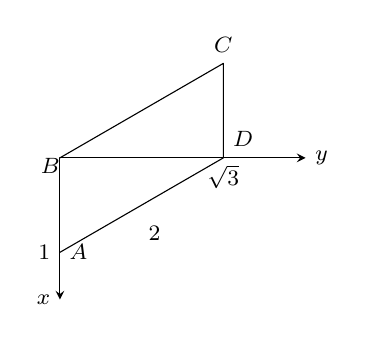
\begin{tikzpicture}[scale=1.2,font=\footnotesize,line join=round, line cap=round,>=stealth]
			\draw[->] (0,0) -- (2.6,0) node[right]{ $y$};
			\draw[->] (0,0) -- (0,-1.5) node[left]{$x$};
			\draw (.1,.1) node[below left]{$B$}
			(1,-.8) node{$2$}
			(0,-1) node[left]{$1$}
			(0,-1) node[right]{$A$}
			(1.73,-0.2) node[]{$\sqrt{3}$}
			(1.73,.2) node[right]{$D$}
			(1.73,1.2) node[]{$C$};
			\draw (0,-1)--(1.73,0)--(1.73,1)--(0,0);
			\end{tikzpicture}}
		\noindent 
		Xét hệ trục tọa độ $Oxyz$, sao cho gốc $O$ trùng với $B$, trục $Ox$ trùng với tia $BA$, trục $Oy$ trùng với tia $BD$, trục $Oz$ trùng với tia $BS$.\\
		Ta có $B(0;0;0)$, $A(1;0;0)$, $C(-1;\sqrt{3};0)$, $D(0;\sqrt{3};0)$, $S(0;0;\sqrt{3})$.\\
		$\vec{SD}=(0;\sqrt{3};\sqrt{3})\Rightarrow \vec{u}=(0;1;-1)$ là một véc-tơ chỉ phương của đường thẳng $SD$.\\
		$\vec{SA}=(1;0;-\sqrt{3})$, $\vec{SC}=(-1;\sqrt{3};-\sqrt{3})\Rightarrow [\vec{SA},\vec{SC}]=(3;2\sqrt{3};\sqrt{3})\Rightarrow \vec{n}=(\sqrt{3};2;1)$ là một véc-tơ pháp tuyến của mặt phẳng $(SAC)$. Vì $\alpha$ là góc tạo bởi $SD$ và mặt phẳng $(SAC)$ nên
		$$\sin \alpha =|\cos(\vec{u},\vec{n})|=\dfrac{|0+2-1|}{\sqrt{2}\cdot \sqrt{8}}=\dfrac{1}{4}.$$
	}
\end{ex}
\begin{ex}%[Đề TT lần 1, Chuyên Nguyễn Thị Minh Khai, Sóc Trăng 2018]%[Hung Tran,12EX-8]]%[2H3K4-1]
	\immini{Cho hình lăng trụ tam giác $ABC.A'B'C'$ có đáy $ABC$ là tam giác vuông tại $A, AB=3,AC=4,AA'=\dfrac{\sqrt{61}}{2}$; hình chiếu của $B'$ trên mặt phẳng $(ABC)$ là trung điểm cạnh $BC$. Gọi $M$ là trung điểm cạnh $A'B'$ (tham khảo hình vẽ bên). Cô-sin của góc tạo bởi hai mặt phẳng $(AMC')$ và $(A'BC)$ bằng
		\choice
		{\True $\dfrac{33}{\sqrt{3157}}$}
		{$\dfrac{11}{\sqrt{3157}}$}
		{$\dfrac{33}{\sqrt{3517}}$}
		{$\dfrac{\sqrt{13}}{65}$}
	}{\begin{tikzpicture}[scale=.6]
		\tkzDefPoints{0/0/A, 2/-3/B, 7/0/C, -1/5/z}
		\tkzDefMidPoint(C,A)
		\tkzGetPoint{H}
		\tkzDefMidPoint(C,B)
		\tkzGetPoint{N}
		\tkzLabelPoints[below](N)
		\coordinate(A') at($(H)+(z)$);
		\tkzLabelPoints[above](A')
		\tkzDefPointBy[translation=from A to A'](B)
		\tkzGetPoint{B'}\tkzLabelPoints[below right](B')
		\tkzDefPointBy[translation=from A to A'](C)
		\tkzGetPoint{C'}\tkzLabelPoints[above](C')
		\tkzDefPointBy[translation=from A to A'](C)
		\tkzDefMidPoint(A',B')\tkzGetPoint{M}\tkzLabelPoints[above right](M)
		\tkzDrawPolygon(A',B',C')
		\tkzDrawPoints(A,B,C,A',B',C',M,N)
		\tkzDrawSegments(A,B B,C A,A' B,B' C,C' B,A' A,M B',N C',M)
		\tkzDrawSegments[dashed](A,C A,H C',A A',C)
		\tkzLabelPoints[below right](B,C)
		\tkzLabelPoints[left](A)
		\tkzLabelSegment[above left](A,C){$4$}
		\tkzLabelSegment[below](A,B){$3$}
		\tkzLabelSegment[left](A,A'){$\dfrac{\sqrt{61}}{2}$}
		\end{tikzpicture}}
	\loigiai{
		\immini{Chọn hệ trục tọa độ gốc $A$ như hình vẽ.\\
			Khi đó $A(0;0;0),B(3;0;0),C(0;4;0)$.\\
			Gọi $N$ là trung điểm $BC\Rightarrow N\left(\dfrac{3}{2};2;0\right)$.\\
			$NB'=\sqrt{BB'^2-BN^2}=3\Rightarrow B'\left(\dfrac{3}{2};2;3\right)$.\\
			Ta có $\overrightarrow{AA'}=\overrightarrow{BB'}\Rightarrow A'\left(-\dfrac{3}{2};2;3\right)$.\\
			Tương tự $\overrightarrow{CC'}=\overrightarrow{BB'}\Rightarrow C'\left(-\dfrac{3}{2};6;3\right)$.\\
			Khi đó $M(0;2;3)$.\\
			$\overrightarrow{AM}=(0;2;3);\overrightarrow{AC'}=\left(-\dfrac{3}{2};6;3\right)$\\
			$\Rightarrow \left[\overrightarrow{AM},\overrightarrow{AC'}\right]=\left(-12;-\dfrac{9}{2};3\right)$.\\
			$\overrightarrow{A'B}=\left(\dfrac{9}{2};-2;-3\right);\overrightarrow{A'C}=\left(\dfrac{3}{2};2;-3\right)$\\
			$\Rightarrow \left[\overrightarrow{A'B},\overrightarrow{A'C}\right]=\left(12;9;12\right)$.\\
		}{\begin{tikzpicture}[scale=.6]
			\tkzDefPoints{0/0/A, 2/-3/B, 7/0/C, -1/6/z, 0/8/Z}
			\tkzDefMidPoint(C,A)
			\tkzGetPoint{H}
			\tkzDefMidPoint(C,B)
			\tkzGetPoint{N}
			\tkzLabelPoints[below](N)
			\coordinate(A') at($(H)+(z)$);
			\tkzLabelPoints[above](A')
			\tkzDefPointBy[translation=from A to A'](B)
			\tkzGetPoint{B'}\tkzLabelPoints[below right](B')
			\tkzDefPointBy[translation=from A to A'](C)
			\tkzGetPoint{C'}\tkzLabelPoints[above](C')
			\tkzDefPointBy[translation=from A to A'](C)
			\tkzDefMidPoint(A',B')\tkzGetPoint{M}\tkzLabelPoints[above right](M)
			\tkzDefPointBy[homothety=center B ratio -1](A)\tkzGetPoint{X}
			\tkzDefPointBy[homothety=center C ratio -1/2](A)\tkzGetPoint{Y}
			\tkzDrawPolygon(A',B',C')
			\tkzDrawPoints(A,B,C,A',B',C',M,N)
			\tkzDrawSegments(A,B B,C A,A' B,B' C,C' B,A' A,M B',N C',M)
			\tkzDrawSegments[dashed](A,C A,H C',A A',C)
			\tkzLabelPoints[below right](C)
			\tkzLabelPoints[left](A,B)
			\tkzLabelSegment[above left](A,C){$4$}
			\tkzLabelSegment[below](A,B){$3$}
			\tkzLabelSegment[left](A,A'){$\dfrac{\sqrt{61}}{2}$}
			\tkzMarkRightAngles[size=0.3](B,A,C)
			\tkzDrawVectors(B,X C,Y A,Z)
			\tkzLabelPoint[left](X){$x$}
			\tkzLabelPoint[above](Y){$y$}
			\tkzLabelPoint[left](Z){$z$}
			\end{tikzpicture}}
		Hai mặt phẳng $(AMC')$ và $(A'BC)$ lần lượt nhận hai véc-tơ $\overrightarrow{n_1}=(-8;-3;2)$ và $\overrightarrow{n_2}=(4;3;4)$ làm véc-tơ pháp tuyến.\\
		$\Rightarrow\cos \left(\overrightarrow{n_1},\overrightarrow{n_2}\right)=\dfrac{\overrightarrow{n_1}\cdot\overrightarrow{n_2}}{|\overrightarrow{n_1}|\cdot |\overrightarrow{n_2}|}=\dfrac{33}{\sqrt{3157}}$\\
		$\Rightarrow$ Cô-sin của góc tạo bởi hai mặt phẳng $(AMC')$ và $(A'BC)$ bằng $\dfrac{33}{\sqrt{3157}}$.
	}
\end{ex}
\begin{ex}%[Thi thử L2, Liên trường THPT Nghệ An, 2018]%[Đinh Thanh Hoàng, 12EX-9]%[2H3G4-1]
	Cho hình lăng trụ tam giác $ABC.A'B'C'$ có đáy là tam giác $ABC$ vuông tại $A$, $AB=3$, $AC=4$, $AA'=\dfrac{\sqrt{61}}{2}$. Hình chiếu của $B'$ lên mặt phẳng $\left(ABC\right)$ là trung điểm cạnh $BC$, $M$ là trung điểm cạnh$A'B'$. Cosin của góc tạo bởi mặt phẳng $\left(AMC'\right)$ và mặt phẳng $\left(A'BC\right)$ bằng
	\choice
	{$\dfrac{\sqrt{13}}{65}$}
	{$\dfrac{11}{\sqrt{3157}}$}
	{$\dfrac{33}{\sqrt{3517}}$}
	{\True $\dfrac{33}{\sqrt{3157}}$}
	\loigiai{
		\immini{
			Gọi $H$ là trung điểm$BC$, theo giả thiết ta có $B'H\perp \left(ABC\right)$.\\
			Mặt khác ta lại có tam giác $ABC$ vuông tại $A$, $AB=3$, $AC=4$ nên $BC=\sqrt{AB^2+AC^2}=5$.\\
			Xét tam giác vuông $B'BH$ ta có
			$$B'H^2=\sqrt{BB'^2-B'H^2}=3.$$
			Chọn hệ trục tọa độ $Oxyz$ có $A$ trùng với $O$ như hình vẽ\\
			Với$A\left(0;0;0\right)$, $B\left(4;0;0\right)$, $C\left(0;3;0\right)$, khi đó trung điểm $H$ của $BC$ là $H\left(\dfrac{3}{2};2;0\right)$.\\ Mặt khác theo giả thiết ta có $AA'=BB'=\dfrac{\sqrt{61}}{2}$ nên $B'\left(\dfrac{3}{2};2;3\right)$.\\
		}{
			\begin{tikzpicture}[scale=0.7,>=stealth]
			\tkzDefPoints{0/0/A,2/-2/B,6/0/C}
			\coordinate (A') at ($(A)+(2,5)$);
			\coordinate (B') at ($(B)+(2,5)$);
			\coordinate (C') at ($(C)+(2,5)$);
			\tkzDefMidPoint(B,C) \tkzGetPoint{H}
			\tkzDefMidPoint(A',B') \tkzGetPoint{M}
			\tkzDefPointBy[homothety = center A ratio 1.5](B) \tkzGetPoint{X}
			\tkzDrawSegments(A,B B,C A',B' B',C' C',A' B',H A',B A,M M,C' A,A' B,B' C,C')
			\tkzDrawSegments[dashed](A,C A,C' A',C)
			\draw[->] (B) -- (X) node[right] {$x$};
			\draw[->] (C) -- (8,0) node[above] {$y$};
			\draw[->] (A) -- (0,8) node[right] {$z$};
			\tkzDrawPoints(A,B,C,A',B',C',H,M)
			\tkzLabelPoints[left](A)
			\tkzLabelPoints[below](H,C)
			\tkzLabelPoints[below left](B)
			\tkzLabelPoints[above](M,B')
			\tkzLabelPoints[above left](A')
			\tkzLabelPoints[above right](C')
			\tkzMarkRightAngles[size=.4](B',H,C B,A,C)
			\end{tikzpicture}
		}
		\noindent Do $\overrightarrow{BB'}=\overrightarrow{AA'}=\overrightarrow{CC'}$ nên $A'\left(-\dfrac{3}{2};2;3\right)$; $C'\left(-\dfrac{3}{2};6;3\right)\Rightarrow M\left(0;2;3\right)$.\\
		$\overrightarrow{AM}=\left(0;2;3\right)$; $\overrightarrow{AC'}=\left(-\dfrac{3}{2};6;3\right)$ nên vectơ pháp tuyến của $\left(MAC'\right)$ là $\overrightarrow{n}_1=\left[\overrightarrow{AM},\overrightarrow{AC'}\right]=\left(-12;-\dfrac{9}{2};3\right)$.\\
		$\overrightarrow{A'B}=\left(\dfrac{9}{2};-2;-3\right)$; $\overrightarrow{A'C}=\left(\dfrac{3}{2};2;-3\right)$ nên vectơ pháp tuyến của $\left(A'BC\right)$ là $\overrightarrow{n}_2=\left[\overrightarrow{A'B},\overrightarrow{A'C}\right]=\left(12;9;12\right)$.\\
		Gọi $\varphi $ là góc tạo bởi mặt phẳng $\left(AMC'\right)$ và mặt phẳng$\left(A'BC\right)$, ta có\\
		$\cos \varphi =\dfrac{\left| \overrightarrow{n}_1\cdot\overrightarrow{n}_2\right|}{\left| \overrightarrow{n}_1\right|\cdot\left| \overrightarrow{n}_2\right|}=\dfrac{\left| 12\cdot(-12)+9\cdot\left(-\dfrac{9}{2}\right)+12\cdot 3\right|}{\sqrt{\left(-12\right)^2+\left(-\dfrac{9}{2}\right)^2+3^2}\cdot\sqrt{9^2+12^2+12^2}}=\dfrac{33}{\sqrt{3157}}$.
	}
\end{ex}
\begin{ex}%[KSCL Lớp 12, Phả Lại - Hải Dương - 2018]%[Vũ Văn Trường, dự án(12EX-9)]%[2H3K4-1]
	Cho hình chóp $S.ABC$ có đáy là tam giác vuông tại $C, AC=3,BC=1$, $SA$ vuông góc với mặt phẳng đáy, $SA=4$. Gọi $M$ là trung điểm của cạnh $AB$. $H$ là điểm đối xứng với $C$ qua $M$. Tính cô-sin của góc tạo bởi hai mặt phẳng $(SHB)$ và $(SBC)$.
	\choice
	{$\dfrac{3\sqrt{17}}{80}$}
	{$\dfrac{3\sqrt{10}}{85}$}
	{\True $\dfrac{3\sqrt{17}}{85}$}
	{$\dfrac{3\sqrt{10}}{80}$}
	\loigiai{
		\immini{
			Chọn hệ tọa độ $Cxyz$ như hình vẽ, khi đó ta có $C(0;0;0), A(3;0;0), B(0;1;0), S(3;0;4), H(3;1;0)$.\\
			$\overrightarrow{CB}=(0;1;0), \overrightarrow{CS}=(3;0;4)\Rightarrow [\overrightarrow{CB},\overrightarrow{CS}]=(4;0;-3)$\\
			$\overrightarrow{BS}=(3;0;0), \overrightarrow{BH}=(3;-1;4)\Rightarrow [\overrightarrow{BS},\overrightarrow{BH}]=(0;12;3)$\\
			Từ đó suy ra các mặt phẳng $(SBC)$ và $(SHB)$ lần lượt có véc-tơ pháp tuyến là $\overrightarrow{n_1}=(4;0;-3)$ và $\overrightarrow{n_2}=(0;4;1)$.\\
			Gọi $\alpha$ là góc giữa các mặt phẳng $(SBC)$ và $(SHB)$, khi đó $$\cos\alpha =|\cos(\overrightarrow{n_1},\overrightarrow{n_2})|=\dfrac{3}{5\sqrt{17}}=\dfrac{3\sqrt{17}}{85}.$$
		}
		{\begin{tikzpicture}[line cap=round,line join=round,scale=0.65,>=stealth]
			\tkzDefPoints{0/0/A,5/0/C,2/-2/B}
			\coordinate (H) at ($(A)+(B)-(C)$);
			\coordinate (M) at($(A)!0.5!(B)$);
			\coordinate (S) at ($(A)+(0,5)$);
			\coordinate (S') at ($(C)+(0,5)$);
			\coordinate (z) at ($(C)!1.3!(S')$);
			\coordinate (x) at ($(C)!1.7!(A)$);
			\coordinate (y) at ($(C)!1.3!(B)$);
			\tkzInterLL(A,x)(S,H)\tkzGetPoint{I}
			\tkzDrawSegments[->](I,x C,z C,y)
			\tkzDrawSegments(S,B S,C B,C H,B S,H)
			\tkzDrawSegments[dashed](C,H C,I A,B S,A)
			\tkzMarkRightAngle(S,A,B)
			\tkzMarkRightAngle(S,A,D)
			\tkzMarkRightAngle(A,C,B)
			\tkzLabelPoints[above](S)
			\tkzLabelPoints[above left](A,x)
			\tkzLabelPoints[below](B,y)
			\tkzLabelPoints[below left=-0.1](M)
			\tkzLabelPoints[left](H)
			\tkzLabelPoints[right](C,z)
			\tkzDrawPoints(A,B,C,S,H,M)
			\end{tikzpicture}
		}
	}
\end{ex}

%C:\Users\Lenovo\Documents\ID6[18-19]\[ID6]\[2H]\[2H3]\[2H3-4]\2H3K4-1.tex
\begin{ex}%[Đề Thi thử, Sở GD-ĐT Quảng Bình 2018]%[Đỗ Đường Hiếu, (dự án 12EX-10)]%[2H3K4-1]
	Cho hình chóp $S.ABC$ có $\triangle ABC$ vuông tại $B$, $AB=1$, $BC=\sqrt{3}$, $\triangle SAC$ đều, mặt phẳng $(SAC)$ vuông góc với mặt phẳng đáy. Gọi $\alpha$ là số đo của góc giữa hai mặt phẳng $(SAB)$ và $(SBC)$. Giá trị $\cos \alpha$ bằng
	\choice
	{\True $\dfrac{\sqrt{65}}{65}$}
	{$\dfrac{\sqrt{65}}{10}$}
	{$\dfrac{2\sqrt{65}}{65}$}
	{$\dfrac{\sqrt{65}}{20}$}
	\loigiai{
		\immini{
			Gọi $H$ là trung điểm của $AC$, khi đó $SH\perp AC \Rightarrow SH\perp (ABC)$.\\
			Ta có $AC=\sqrt{AB^2+BC^2}=2$, suy ra $SH=\dfrac{AC\sqrt{3}}{2}=\sqrt{3}$.\\
			Đặt hệ trục tọa độ $Oxyz$ như hình vẽ.\\
			Ta có $B(0;0;0)$, $A(1;0;0)$, $C(0;\sqrt{3};0)$, $H\left(\dfrac{1}{2};\dfrac{\sqrt{3}}{2};0\right)$ và $S\left(\dfrac{1}{2};\dfrac{\sqrt{3}}{2};\sqrt{3}\right)$.
			\begin{itemize}
				\item $\overrightarrow{BA}=(1;0;0)$, $\overrightarrow{BS}=\left(\dfrac{1}{2};\dfrac{\sqrt{3}}{2};\sqrt{3}\right)$,\\
				$\left[\overrightarrow{BA},\overrightarrow{BS}\right]=\left(0;-\sqrt{3};\dfrac{\sqrt{3}}{2}\right)$.\\
				Suy ra, mặt phẳng $(SAB)$ có véc-tơ pháp tuyến $\overrightarrow{n}_1=(0;-2;1)$.
				\item $\overrightarrow{BC}=(0;\sqrt{3};0)$, $\overrightarrow{BS}=\left(\dfrac{1}{2};\dfrac{\sqrt{3}}{2};\sqrt{3}\right)$,\\
				$\left[\overrightarrow{BC},\overrightarrow{BS}\right]=\left(3;0;-\dfrac{\sqrt{3}}{2}\right)$.\\
				Suy ra, mặt phẳng $(SAC)$ có véc-tơ pháp tuyến $\overrightarrow{n}_2=(2\sqrt{3};0;-1)$.
			\end{itemize}
		}{
			\begin{tikzpicture}[>=stealth, scale=.8]
			\coordinate (B) at (0,0);
			\coordinate (A) at (1.5,-1.5);
			\coordinate (C) at (4,0);
			\coordinate (H) at ($(A)!.5!(C)$);
			\coordinate (X) at ($(B)!1.5!(A)$);
			\coordinate (Y) at ($(B)!1.3!(C)$);
			\coordinate (S) at ($(H)+(0,4)$);
			\coordinate (Z) at ($(B)+(0,5)$);
			\draw (H)--(S)--(B)--(A)--(S)--(C)--(A);
			\draw[dashed] (B)--(C);
			\draw[->] (A)--(X) node[below] {$x$};
			\draw[->] (C)--(Y) node[below] {$y$};
			\draw[->] (B)--(Z) node[right] {$z$};
			\tkzDrawPoints(A,B,C,S,H);
			\tkzLabelPoints[below](A,B,C,H);
			\tkzLabelPoints[above](S);
			\tkzMarkRightAngles(A,B,C S,H,A);
			\draw(-.2,.2) node {$O$};
			\end{tikzpicture}
		}
		Do đó
		\begin{eqnarray*}
			\cos \alpha =\dfrac{\left|\overrightarrow{n}_1\cdot \overrightarrow{n}_2\right|}{\left|\overrightarrow{n}_2\right|\cdot\left|\overrightarrow{n}_2\right|}=\dfrac{\left|0\cdot (2\sqrt{3})+(-2)\cdot 0+1\cdot (-1)\right|}{\sqrt{0^2+(-2)^2+1^2}\cdot \sqrt{(2\sqrt{3})^2+0^2+(-1)^2}}=\dfrac{\sqrt{65}}{65}.
		\end{eqnarray*}
	}
\end{ex}
\begin{ex}%[Thi thử L6, lớp 12, Chuyên Thái Bình, Thái Bình 2018]%[Võ Tấn Đạt, 12EX10]%[2H3G4-1]
	Cho hình lăng trụ đứng $ABC.A'B'C'$ có đáy là tam giác $ABC$ vuông cân tại $A$, cạnh $BC=a\sqrt{6}$. Góc giữa mặt phẳng $(AB'C)$ và mặt phẳng $(BCC'B')$ bằng $60^{\circ}$. Tính thể tích khối đa diện $AB'CA'C'$.
	\choice
	{$\dfrac{\sqrt{3}a^3}{2}$}
	{\True $\sqrt{3}a^3$}
	{$\dfrac{\sqrt{3}a^3}{3}$}
	{$\dfrac{3\sqrt{3}a^3}{2}$}
	\loigiai{
		\immini{Gọi $h \; (h>0)$ là chiều cao lăng trụ. Tam giác $ABC$ vuông cân tại $A$ nên ta tính được $AB=AC=a\sqrt{3}$.\\
			Chọn hệ trục tọa độ $Oxyz$ sao cho\\
			$A \equiv O$, tia $AB$ trùng $Ox$, tia $AC$ trùng $Oy$, tia $AA'$ trùng $Oz$.\\ Khi đó ta có
			$A(0;0;0)$, $B(a\sqrt{3};0;0),$ $C(0;a\sqrt{3};0),$ $B'(a\sqrt{3};0;h)$ $\Rightarrow \overrightarrow{AC}=(0;a\sqrt{3};0)$, $\overrightarrow{BC}=(-a\sqrt{3};$ $a\sqrt{3};0),$ $\overrightarrow{B'C}~=~(a\sqrt{3};-a\sqrt{3};h)$.\\
			Như vậy $\overrightarrow{n_1}=\left[\overrightarrow{AC},\overrightarrow{B'C}\right]=(ha\sqrt{3};0;-3a^2)$ là một véc tơ pháp tuyến của mặt phẳng $(AB'C)$ và $\overrightarrow{n_2}~=~\left[\overrightarrow{BC},\overrightarrow{B'C}\right]~=~(ha\sqrt{3};ha\sqrt{3};0)$ là một véc tơ pháp tuyến của mặt phẳng $(BCC'B')$.}{\begin{tikzpicture}[scale=.5,>=stealth]
			\tkzDefPoints{0/0/A, -3/-3/B, 3/-3/C, 0/8/A', -3/5/B', 3/5/C', -4.5/-4.5/I, 4.5/-4.5/G, -3/1/H, -1.5/-1.5/M, 1.5/-1.5/N, 0/-3/K, 0/9.5/S}
			\draw(0,9.5) node[left]{$z$};
			\draw(-4.5,-4.5) node[left]{$x$};
			\draw(4.5,-4.5) node[right]{$y$};
			\tkzText[left](-3,1){$h$}
			\tkzText[left](-1.3,-0.8){$a\sqrt{3}$}
			\tkzText[right](1.3,-0.8){$a\sqrt{3}$}
			\tkzText[below](0,-3){$a\sqrt{6}$}
			\tkzDrawSegments[->](B,I);
			\tkzDrawSegments[->](C,G);
			\tkzDrawSegments[->](A',S);
			\tkzDrawSegments[dashed](B,A A,C B',A A,A');
			\tkzDrawSegments(B',A' A',C' C',B' B,C B,B' C,C' B',C);
			\tkzLabelPoints[right](C,C');
			\tkzLabelPoints[above right](A);
			\tkzLabelPoints[above left](A');
			\tkzLabelPoints[left](B',B);
			\draw(B) circle (1pt) ;\draw(A') circle (1pt) ;\draw(A) circle (1pt) ;
			\draw(C) circle (1pt) ;\draw(B') circle (1pt) ;\draw(C') circle (1pt) ;
			\tkzDrawPoints(A,B,C,A',B',C')
			\end{tikzpicture}}
		\noindent Theo giả thiết
		\begin{align*}
		\left((AB'C),(BCC'B')\right)=60^{\circ}&\Rightarrow \cos \left((AB'C),(BCC'B')\right)= \cos (\overrightarrow{n_1},\overrightarrow{n_2})=\dfrac{1}{2}\\
		&\Leftrightarrow \dfrac{1}{2}=\dfrac{\left|\overrightarrow{n_1}\cdot \overrightarrow{n_2}\right|}{\left|\overrightarrow{n_1}\right|\cdot \left|\overrightarrow{n_2}\right|}=\dfrac{3a^2h^2}{\sqrt{3a^2h^2+9a^4}\cdot \sqrt{6a^2h^2}}\\
		&\Leftrightarrow \sqrt{3a^2h^2+9a^4}\cdot \sqrt{6a^2h^2}=6a^2h^2\\ &\Leftrightarrow 3a^2h^2+9a^4=6a^2h^2\\
		&\Leftrightarrow h=a\sqrt{3}.
		\end{align*}
		Do đó $V_{ABC.A'B'C'}=a\sqrt{3}\cdot \dfrac{1}{2}(a\sqrt{3})^2=\dfrac{3\sqrt{3}a^3}{2}, V_{B'.ABC}=\dfrac{1}{3}a\sqrt{3}\cdot \dfrac{1}{2}(a\sqrt{3})^2=\dfrac{\sqrt{3}a^3}{2}. \\
		\Rightarrow V_{AB'CA'C}=V_{ABC.A'B'C'}-V_{B'.ABC}=\sqrt{3}a^3$.
	}
\end{ex}
\begin{ex}%[Đề TT THPT Quốc gia tháng 6, 2017 - 2018, cụm Tp. Vũng Tàu]%[Nguyễn Hoàng Hải, dự án 12EX11]%[2H3K4-1]
	Cho hình chóp $S.ABCD$ có đáy là hình vuông, tam giác $SAD$ vuông cân tại $S$ và thuộc mặt phẳng vuông góc với $(ABCD)$. Gọi $\alpha $ là góc hợp bởi hai mặt phẳng $(SBC)$ và $(SCD)$. Giá trị của $\tan \alpha$ là
	\choice
	{$ \dfrac{\sqrt{6}}{3} $}
	{$ \dfrac{\sqrt{5}}{2} $}
	{\True$ \dfrac{\sqrt{6}}{2} $}
	{$ \dfrac{\sqrt{5}}{3} $}
	\loigiai{
		\immini{
			Gọi $ O $ là trung điểm $ AD $, $ a $ là độ dài cạnh hình vuông. \\
			Gắn hệ tọa độ $ Oxyz $ như hình vẽ. Khi đó
			$$ S\left( 0;0;\dfrac{a}{2} \right),B\left( a;-\dfrac{a}{2};0 \right),C\left( a;\dfrac{a}{2};0 \right), D\left( 0;\dfrac{a}{2};0 \right) $$
			Ta có
			\begin{itemize}
				\item $ \vec{SC}\left( a;\dfrac{a}{2};-\dfrac{a}{2} \right) $.
				\item $ \vec{SB}\left( a;-\dfrac{a}{2};-\dfrac{a}{2} \right) $.
				\item $ \vec{SD}\left( 0;\dfrac{a}{2};-\dfrac{a}{2} \right) $.
			\end{itemize}
		}{
			\begin{tikzpicture}[>=stealth,x=1cm,y=1cm,scale=1]
			\tkzInit[ymin=-1,ymax=10,xmin=-1,xmax=15]
			%\tkzClip
			%\tkzGrid
			%\tkzAxeXY
			\tkzSetUpPoint[color=black,fill=white,size=6]
			\tkzDefPoints{0/0/A,3/0/B,-2/-2/D}
			\tkzDefPointBy[translation=from A to B](D)\tkzGetPoint{C}
			\tkzDefMidPoint(A,D)\tkzGetPoint{I}
			\coordinate (S) at ($(-1,1)$);
			\tkzDefMidPoint(C,B)\tkzGetPoint{J}
			\coordinate (x) at ($(J)+(1,0)$);
			\coordinate (y) at ($(I)+1.1*(D)$);
			\tkzDefPointBy[homothety=center I ratio 1.3](S)\tkzGetPoint{z}
			\draw($(I)$)node[below right = -0.1 and -0.1]{$O$};
			\tkzDrawSegments[style=dashed](A,B A,D S,A S,I I,J)
			\tkzDrawSegments(B,C C,D S,B S,C S,D J,x)
			\tkzDrawSegments[->](J,x D,y S,z)
			\tkzDrawPoints(A,B,C,D,I,S)
			\tkzLabelPoints[left](S)
			\tkzLabelPoints[right](x)
			\tkzLabelPoints[above](z)
			\tkzLabelPoints[above left]()
			\tkzLabelPoints[above right](B)
			\tkzLabelPoints[below](D,C,y)
			\tkzLabelPoints[below left]()
			\tkzLabelPoints[below right = -0.1 and -0.1](A)
			\end{tikzpicture}
		}
		\begin{itemize}
			\item $ \left[ \vec{SC},\vec{SB} \right]=a^2\left( -\dfrac{1}{2};0;-1 \right) $,
			vậy $ (SBC) $ có một véc-tơ pháp tuyến là $ \vec{n}_1=\left( -\dfrac{1}{2};0;-1 \right) $.
			\item $ \left[ \vec{SC},\vec{SD} \right]=a^2\left( 0;\dfrac{1}{2};\dfrac{1}{2} \right) $, vậy $ (SCD) $ có một véc-tơ pháp tuyến là $ \vec{n}_2=\left( 0;\dfrac{1}{2};\dfrac{1}{2} \right) $.
		\end{itemize}
		Ta có $ \cos(\vec{n}_1,\vec{n}_2)=\dfrac{\vec{n}_1\cdot\vec{n}_2}{|\vec{n}_1|\cdot|\vec{n}_2|}=-\dfrac{\sqrt{2}}{\sqrt{5}} \Rightarrow \cos\alpha=\dfrac{\sqrt{2}}{\sqrt{5}} \Rightarrow \sin\alpha=\dfrac{\sqrt{3}}{\sqrt{5}}$. \\
		Vậy $ \tan\alpha=\dfrac{\sin\alpha}{\cos\alpha}=\dfrac{\sqrt{6}}{2} $.
	}
\end{ex}
\begin{ex}%[Thi thử L3, Bắc Yên Thành, Nghệ An, 2018]%[Nguyễn Tiến Thùy, 12EX-11]%[2H3K4-1]
	Cho hình chóp $S.ABCD$ có đáy $ABCD$ là hình vuông cạnh bằng $2$, $SA\perp (ABCD)$ và $SA=2$. Gọi $M$, $N$, $P$ lần lượt là trung điểm của $AB$, $BC$, $CS$. Tính cosin của góc tạo bởi mặt phẳng $(MNP)$ và $(SBD)$.
	\choice
	{$\dfrac{\sqrt{2}}{3}$}
	{$\dfrac{1}{\sqrt{3}}$}
	{\True $\dfrac{1}{3}$}
	{$\dfrac{2}{3}$}
	\loigiai{
		\immini{
			Gắn khối chóp vào hệ tọa độ $Oxyz$ với $A(0;0;0)$, $B(2;0;0)$, $D(0;2;0)$, $S(0;0;2)$, $C(2;2;0)$.\\
			Do $M$, $N$, $P$ lần lượt là trung điểm của $AB$, $BC$, $SC$ suy ra $M(1;0;0)$, $N(2;1;0)$, $P(1;1;1)$.\\
			Ta có phương trình dạng chắn của mặt phẳng $(SBD)$ là
			$$\dfrac{x}{2}+\dfrac{y}{2}+\dfrac{z}{2}=1,$$
			từ đó suy ra mặt phẳng $(SBD)$ có véc-tơ pháp tuyến là $\vec{n}_1=(1;1;1)$.
		}{
			\begin{tikzpicture}[scale=1, line join=round, line cap=round]
			\tkzDefPoints{0/0/A,-1.3/-1.6/B,2.5/-1.6/C}
			\coordinate (D) at ($(A)+(C)-(B)$);
			\coordinate (S) at ($(A)+(0,3)$);
			\coordinate (M) at ($(A)!0.5!(B)$);
			\coordinate (N) at ($(B)!0.5!(C)$);
			\coordinate (P) at ($(C)!0.5!(S)$);
			\tkzDrawPolygon(S,B,C,D)
			\tkzDrawSegments(S,C N,P)
			\tkzDrawSegments[dashed](A,S A,B A,D M,N M,P B,D)
			\tkzDrawPoints[fill=black,size=4](D,C,A,B,S,M,N,P)
			\tkzLabelPoints[above](S)
			\tkzLabelPoints[below](B,C,N)
			\tkzLabelPoints[above left](A,M)
			\tkzLabelPoints[right](D,P)
			\tkzMarkRightAngles[size=0.2,fill=gray!10](B,A,D S,A,B S,A,D)
			\end{tikzpicture}
		}
		\noindent Mặt khác, mặt phẳng $(MNP)$ có hai véc-tơ chỉ phương là $\vec{MN}=(1;1;0)$ và $\vec{MP}=(0;1;1)$, từ đó suy ra $\vec{n}_2=\left[\vec{MN},\vec{MP}\right]=(1;-1;1)$ là véc-tơ pháp tuyến của mặt phẳng $(MNP)$.\\
		Gọi $\varphi$ là góc tạo bởi hai mặt phẳng $(MNP)$ và $(SBD)$, suy ra
		\begin{center}
			$\cos\varphi=\dfrac{\left|\vec{n}_1\cdot\vec{n}_2\right|}{\left|\vec{n}_1\right|\cdot\left|\vec{n}_2\right|}=\dfrac{1}{\sqrt{3}\cdot\sqrt{3}}=\dfrac{1}{3}$.
		\end{center}
	}
\end{ex}
\begin{ex}%[Thi thử L3, THPT Hậu Lộc 2, Thanh Hóa, 2018]%[Hưng Nguyễn, dự án 12-EX-11]%[2H3G4-1]
	Cho hình chóp $S.ABC$ có $SA$ vuông góc với mặt phẳng đáy. Gọi $M$ là trung điểm của $BC$ và $H$ là trung điểm của $AM$. Biết $HB=HC$, $\widehat{HBC}=30^\circ$; góc giữa mặt phẳng $(SHC)$ và mặt phẳng $(HBC)$ bằng $60^\circ$. Tính cô-sin của góc giữa đường thẳng $BC$ và mặt phẳng $(SHC)$.
	\choice
	{\True $\dfrac{\sqrt{13}}{4}$}
	{$\dfrac{\sqrt{3}}{2}$}
	{$\dfrac{\sqrt{3}}{4}$}
	{$\dfrac{1}{2}$}
	\loigiai{
		\immini
		{
			$HB=HC$ nên tam giác $HBC$ cân tại $H$, suy ra $HM\perp BC$.\\
			Trong mặt phẳng $(ABC)$ dựng $AK\perp HC\Rightarrow HC\perp (SAK)$.\\
			Mà góc giữa mặt phẳng $(SHC)$ và $(ABC)$ bằng $60^\circ$ nên $\widehat{SKA}=60^\circ$.\\
			Giả sử $BC=a$.\\
			$\Rightarrow BM=\dfrac{a}{2}\Rightarrow AH=HM=BM\cdot \tan 30^\circ=\dfrac{a\sqrt{3}}{6}$\\
			$\Rightarrow AK=AH\cdot \sin 60^\circ=\dfrac{a}{4}\Rightarrow SA=AK\cdot \tan 60^\circ=\dfrac{a\sqrt{3}}{4}$.\\
		}
		{
			\begin{tikzpicture}[scale=.6, font=\footnotesize, line join=round, line cap=round,>=stealth]
			\tkzDefPoints{0/0/A,2/-2/B,6/0/C,0/5/S}
			\tkzDefMidPoint(C,B)\tkzGetPoint{M}
			\tkzDefMidPoint(A,M)\tkzGetPoint{H}
			\tkzDefPointBy[homothety=center C ratio 1.25](H)\tkzGetPoint{K}
			\tkzDefPointBy[homothety=center A ratio 1.2](M)\tkzGetPoint{M'}
			\tkzDefPointBy[translation= from B to C](A) \tkzGetPoint{A'}
			\tkzDefPointBy[homothety=center A ratio .7](A')\tkzGetPoint{A''}
			\tkzDefPointBy[homothety=center A ratio 1.2](S)\tkzGetPoint{S'}
			\tkzDrawSegments(A,B B,C C,S S,A S,B)
			\tkzDrawSegments[dashed](A,C S,K K,C A,M A,K)
			\tkzLabelPoints[left](A,S)
			\tkzLabelPoints[right](C) \tkzLabelPoints[below](M,B,K,H)
			\tkzDrawPoints[fill=black](A,B,C,S,H,K,M)
			\tkzMarkRightAngle(A,K,C)
			\draw [->] (M)--(M') node[below]{$x$};
			\draw [->] (S)--(S') node[left]{$z$};
			\draw [->,dashed] (A)--(A'') node[below]{$y$};
			\end{tikzpicture}
		}
		\noindent Trang bị hệ trục tọa độ $Axyz$ với $A(0;0;0)$, $S \left(0;0;\dfrac{\sqrt{3}}{4}\right)$, $H \left(\dfrac{\sqrt{3}}{6};0;0\right)$, $C \left(\dfrac{\sqrt{3}}{3};\dfrac{1}{2};0\right)$, $B \left(\dfrac{\sqrt{3}}{3};\dfrac{-1}{2};0\right)$.\\
		$\Rightarrow \overrightarrow{SH}=\left(\dfrac{\sqrt{3}}{6};0;\dfrac{-\sqrt{3}}{4}\right)$, $\overrightarrow{HC}=\left(\dfrac{\sqrt{3}}{6};\dfrac{1}{2};0\right)$, $\overrightarrow{BC}=(0;1;0)$.\\
		Từ đó suy ra mặt phẳng $(SHC)$ nhận $\overrightarrow{n}=(3\sqrt{3};-3;2\sqrt{3})$ là véc-tơ pháp tuyến.\\
		Ta có $\sin (BC,(SHC))=|\cos (\overrightarrow{n},\overrightarrow{BC})|=\left|\dfrac{-3}{\sqrt{48}}\right|=\dfrac{\sqrt{3}}{4}\Rightarrow \cos (BC,(SHC))=\dfrac{\sqrt{13}}{4}$.
	}
\end{ex}
\begin{ex}%[Đề HK2, 2018, Sở Đồng Nai]%[Trần Quang Thạnh, dự án EX9]%[2H3K4-1]
	Cho hình lập phương $MNPQ.M'N'P'Q'$ có $E, F, G$ lần lượt là trung điểm của $NN', PQ, M'Q'$ Tính góc giữa hai đường thẳng $EG$ và $P'F$.
	\choice
	{$60^{\circ} $}
	{$30^{\circ} $}
	{\True $90^{\circ} $}
	{$45^{\circ} $}
	\loigiai{
		\immini{Chọn hệ trục tọa độ $Oxyz$ sao cho $M(0;0;0)$, $N(1;0;0)$, $Q(0;1;0)$ và $M'(0;0;1)$. Lúc đó $P(1;1;0), N'(1;0;1), Q'(0;1;1)$ và $P'(1;1;1)$.\\
			Vì $E, F, G$ lần lượt là trung điểm $NN', PQ$ và $M'Q'$ nên $E\left(1;0;\dfrac{1}{2}\right)$, $F\left(\dfrac{1}{2};1;0\right)$ và $G\left(0;\dfrac{1}{2};1\right)$.\\
			Suy ra $\vec{EG}=\left(-1;\dfrac{1}{2};\dfrac{1}{2}\right)$, $\vec{P'F}=\left(-\dfrac{1}{2};0;-1\right)$, do đó $\vec{EG}\cdot \vec{P'F}=0$ hay $(EG,P'F)=90^{\circ}$.}{\begin{tikzpicture}[line cap=round,line join=round,scale=1.5]%[Mai Hà Lan] %1.20
			%-------------- Đáy ABCD
			\tkzDefPoints{0/0/A, -0.5/-1/B, 2/0/D}
			\coordinate (C) at ($(B)+(D)-(A)$);
			%-------------- Đáy A'B'C'D'
			\tkzDefPointBy[rotation = center A angle 90](D) \tkzGetPoint{A'} %Phép quay tâm A, góc quay 90 độ, biến D thành A'
			\coordinate (B') at ($(B)+(A')-(A)$);
			\coordinate (D') at ($(D)+(A')-(A)$);
			\coordinate (C') at ($(B')+(D')-(A')$);
			%---------------
			\tkzDrawSegments[dashed](A,B A,D A,A')
			\tkzDrawPolygon(A',B',C',D')
			\tkzDrawPolygon(B,C,C',B')
			\tkzDrawSegments(D,D' C,D)
			\tkzDrawPoints(A,B,C,D,A',B',C',D')
			\tkzLabelPoint(A){$M$}
			\tkzLabelPoint(B){$N$}
			\tkzLabelPoint(C){$P$}
			\tkzLabelPoint(D){$Q$}
			\tkzLabelPoint(A'){$M'$}
			\tkzLabelPoint(B'){$N'$}
			\tkzLabelPoint(C'){$P'$}
			\tkzLabelPoint(D'){$Q'$}
			%\tkzLabelPoints(A,B,C,D,A',B',C',D')
			\tkzDefMidPoint(B,B') \tkzGetPoint{E}
			\tkzDefMidPoint(C,D) \tkzGetPoint{F}
			\tkzDefMidPoint(A',D') \tkzGetPoint{G}
			\tkzLabelPoints[above](G)
			\tkzLabelPoints[right](E,F)
			\tkzDrawSegments[dashed](E,G)
			\tkzDrawSegments(C',F)
			\tkzDrawPoints(G,E)
			\end{tikzpicture}}
	}
\end{ex}
\begin{ex}%[TT THPT Quốc Gia (2017-2018), THPT Hồng Lĩnh, Hà Tĩnh]%[Bùi Mạnh Tiến, dự án (12EX-8)]%[2H3K4-1]
	Cho hình chóp $S.ABC$ có $SC\perp (ABC)$ và tam giác $ABC$ vuông tại $B$. Biết $AB=a,AC=a\sqrt{3},SC=a\sqrt{12}$. Sin của góc giữa hai mặt phẳng $(SAB),(SAC)$ bằng
	\choice
	{\True $\sqrt{\dfrac{5}{7}}$}
	{$1$}
	{$\dfrac{5\sqrt{14}}{42}$}
	{$\sqrt{\dfrac{2}{3}}$}
	\loigiai{
		\immini{
			Ta có tam giác $ABC$ vuông tại B nên:\\ $BC=\sqrt{AC^2-AB^2}=a\sqrt{2}$.\\
			Ta dựng trục tọa độ $Oxyz$ như hình vẽ bên. Chuẩn hóa $a = 1$.\\
			Tọa độ các điểm như sau:\\
			$B(0;0;0),A(1;0;0), C(0;\sqrt{2};0),S(0;\sqrt{2};\sqrt{12})$.\\
			$\vec{SA}=(1;-\sqrt{2};-\sqrt{12});\vec{SB}=(0;-\sqrt{2};-\sqrt{12})$.\\
			$\vec{SC}=(0;0;-\sqrt{12})$.\\
			$\left[\vec{SA},\vec{SB}\right]=(0;\sqrt{12};-\sqrt{2})$\\
			$\Rightarrow \vec{n_{SAB}}=(0;\sqrt{6};-1)$.
			$\left[\vec{SA},\vec{SC}\right]=(\sqrt{24};\sqrt{12};0)$\\
			$\Rightarrow \vec{n_{SAB}} = (\sqrt{2};1;0)$.
		}
		{
			\begin{tikzpicture}[>=stealth, line join=round, line cap = round]
			\tkzDefPoints{1/0/C, 2/-2/B, 6/0/A, 1/4/S, 7/0.5/X, 0/2/Y, 2/5/Z}
			\tkzDefMidPoint(S,C)\tkzGetPoint{M}
			\tkzDrawSegments(S,A S,B S,C)
			\tkzDrawSegments[dashed](A,C)
			\tkzDrawVector(B,Z)
			\tkzDrawVector(B,X)
			\tkzDrawVector(B,Y)
			\tkzLabelPoints[above](S)
			\tkzLabelPoints[left](C)
			\tkzLabelPoints[right](A)
			\draw (B) node[below] {$B\equiv O$};
			\draw (X) node[right] {$x$};
			\draw (Y) node[left] {$y$};
			\draw (Z) node[right] {$z$};
			\tkzDrawPoints(S,A,B,C)
			\tkzMarkRightAngles(A,B,C S,C,A S,C,B)
			\tkzLabelSegment[below right](A,B){$a$}
			\tkzLabelSegment[above](C,A){$a\sqrt{3}$}
			\tkzLabelSegment[left](S,M){$a\sqrt{12}$}
			\end{tikzpicture}
		}
		\flushleft
		Gọi $\varphi $ là góc giữa hai mặt phẳng $(SAB)$ và $(SAC)$.\\
		$\cos \varphi = \cos ((SAB),(SAC))=\cos (\vec{n_{SAB}},\vec{n_{SAB}})=\dfrac{|\vec{n_{SAB}}\cdot \vec{n_{SAC}}|}{|\vec{n_{SAB}}|\cdot |\vec{n_{SAB}}|}=\dfrac{\sqrt{6}}{\sqrt{3}\sqrt{7}}=\dfrac{\sqrt{2}}{\sqrt{7}}$.\\
		$\Rightarrow \sin \varphi = \sqrt{1-\cos ^2 \varphi }=\sqrt{\dfrac{5}{7}}$.
	}
\end{ex}
\begin{ex}%[Thi thử L3, Bắc Yên Thành, Nghệ An, 2018]%[Nguyễn Tiến Thùy, 12EX-11]%[2H3K4-1]
	Cho hình chóp $S.ABC$ có $SA=SB=SC=AB=AC=a\sqrt{2}$ và $BC=2a$. Góc giữa hai đường thẳng $SC$ và $AB$ là
	\choice
	{$30^\circ$}
	{\True $60^\circ$}
	{$90^\circ$}
	{$45^\circ$}
	\loigiai{
		\immini{
			Dễ dàng chứng minh được các tam giác $ABC$ và $SBC$ là tam giác vuông cân tại $A$ và $S$.\\
			Gọi $H$ là trung điểm của cạnh $BC$, suy ra $H$ là tâm đường tròn ngoại tiếp tam giác vuông $ABC$ và $AH=SH=a$. \\
			Mặt khác, do $SA=SB=SC$ nên $SH$ là trục của đáy $ABC$, tương tự $AH$ là trục của tam giác $SBC$.\\
			Gắn khối chóp vào hệ tọa độ $Oxyz$, với $H(0;0;0)$, $A(a;0;0)$, $C(0;a;0)$, $S(0;0;a)$, $B(0;-a;0)$.
		}{
			\begin{tikzpicture}[scale=1,line join=round,line cap=round]
			\tkzDefPoints{0/0/B,1/-1.5/A,4/0/C}
			\coordinate (H) at ($(B)!0.5!(C)$);
			\coordinate (S) at ($(H)+(0,3)$);
			\tkzDrawPolygon(S,B,A,C)
			\tkzDrawSegments(S,A)
			\tkzDrawSegments[dashed](S,H A,H)
			\tkzDrawSegments[dashed](B,C)
			\tkzDrawPoints[fill=black,size=4](A,B,C,S,H)
			\tkzLabelPoints[above](S)
			\tkzLabelPoints[below](A)
			\tkzLabelPoints[below right](H)
			\tkzLabelPoints[left](B)
			\tkzLabelPoints[right](C)
			\tkzMarkRightAngles[size=0.3,fill=gray!10](S,H,A S,H,C A,H,C)
			\end{tikzpicture}
		}
		\noindent Từ đó ta có $\vec{SC}=(0;a;-a)=a(0;1;-1)$ và $\vec{AB}=(-a;-a;0)=-a(1;1;0)$.\\
		Gọi $\varphi$ là góc giữa hai đường thẳng $SC$ và $AB$, suy ra
		$$\cos\varphi=\dfrac{\left|\vec{SC}\cdot\vec{AB}\right|}{\left|\vec{SC}\right|\cdot\left|\vec{AB}\right|}=\dfrac{1}{\sqrt{2}\cdot\sqrt{2}}=\dfrac{1}{2}.$$
		Từ đó suy ra $\varphi=60^\circ$.
	}
\end{ex}
\begin{ex}%[Thi thử L3, Chuyên Lào Cai, 2018]%[Trần Chiến, dự án 12-EX-11-2018]%[2H3K4-1]
	Cho hình chóp $S.ABCD$ có đáy $ABCD$ là hình vuông cạnh bằng $a$, $SO=a$ và $SO$ vuông góc với mặt đáy $(ABCD)$. Gọi $M$, $N$ là trung điểm của $SA$, $BC$. Gọi $\alpha$ là góc giữa đường thẳng $MN$ và mặt phẳng $(SBD)$. Tính $\cos\alpha$.
	\choice
	{\True $\dfrac{\sqrt{21}}{7}$}
	{$\dfrac{2}{5}$}
	{$\dfrac{\sqrt{5}}{10}$}
	{$\dfrac{2}{\sqrt{7}}$}
	\loigiai{
		\immini{
			Ta chuẩn hóa $a=1$.\\
			Chọn hệ trục tọa độ như hình vẽ với:\\
			$S(0;0;1)$, $A\left(-\dfrac{\sqrt{2}}{2};0;0\right)\Rightarrow M\left(-\dfrac{\sqrt{2}}{4};0;\dfrac{1}{2}\right)$.\\
			$B\left(0;-\dfrac{\sqrt{2}}{2};0\right)$, $C\left(\dfrac{\sqrt{2}}{2};0;0\right)\Rightarrow N\left(\dfrac{\sqrt{2}}{4};-\dfrac{\sqrt{2}}{4};0\right)$.\\
			Suy ra $\overrightarrow{MN}=\left(\dfrac{\sqrt{2}}{2};-\dfrac{\sqrt{2}}{4};-\dfrac{1}{2}\right)$ do đó đường thẳng $MN$ có một véc-tơ chỉ phương là $\overrightarrow{u}=(2;-1;-\sqrt{2})$.\\
			Ta thấy mặt phẳng $(SBD)$ có một véc-tơ pháp tuyến là $\overrightarrow{i}=(1;0;0)$.
		}{
			\begin{tikzpicture}[scale=1, line join=round, line cap=round, >=stealth]
			\tkzDefPoints{0/0/B, 1/1/A, 4/0/C}
			\coordinate (D) at ($(C)-(B)+(A)$);
			\tkzInterLL(A,C)(B,D)\tkzGetPoint{O}
			\coordinate (S) at ($(O)+(0,4)$);
			\tkzDefMidPoint(S,A)\tkzGetPoint{M}
			\tkzDefMidPoint(B,C)\tkzGetPoint{N}
			\coordinate (x) at ($(O)!1.7!(C)$);
			\coordinate (y) at ($(O)!1.5!(D)$);
			\coordinate (z) at ($(O)!1.3!(S)$);
			\tkzDrawSegments(S,B B,C C,D S,C S,D)
			\tkzDrawSegments[->](S,z D,y C,x)
			\tkzDrawSegments[dashed](S,A S,B A,B A,D A,C B,D S,O M,N)
			\tkzLabelPoints[above left](S)
			\tkzLabelPoints[above right](A,x)
			\tkzLabelPoints[below left](B,C)
			\tkzLabelPoints[below](O,N)
			\tkzLabelPoints[right](z,M)
			\tkzLabelPoints[above](D,y)
			\tkzDrawPoints[fill=black](S,A,B,C,D,O,M,N)
			\end{tikzpicture}}
		\noindent Suy ra $\sin\alpha=\dfrac{|2\cdot 1 -1\cdot 0 -\sqrt{2}\cdot 0|}{\sqrt{2^2+(-1)^2+(-\sqrt{2})^2}\cdot \sqrt{1^2+0^2+0^2}}=\dfrac{2}{\sqrt{7}}$.\\
		Vì $\alpha \leq 90^\circ$ nên $\cos\alpha=\dfrac{\sqrt{21}}{7}$.
	}
\end{ex}
\begin{ex}%[Đề KSCL trường THPT chuyên Hùng Vương, Phú Thọ, năm 2018, lần 4]%[Nguyễn Thành Khang, 12-Ex-9]%[2H3B4-1]
	Cho hình chóp $S.ABC$ có $SA=a,SA\perp (ABC)$, tam giác $ABC$ vuông cân đỉnh $A$ và $BC=a\sqrt{2}$. Gọi $M,N$ lần lượt là trung điểm của $SB,SC$. Cô-sin của góc tạo bởi hai mặt phẳng $(MNA)$ và $(ABC)$ bằng
	\choice
	{$\dfrac{\sqrt{3}}{2}$}
	{$\dfrac{\sqrt{2}}{4}$}
	{\True $\dfrac{\sqrt{3}}{3}$}
	{$\dfrac{\sqrt{2}}{6}$}
	\loigiai{
		\immini{
			$\triangle ABC$ vuông cân tại $A$ nên $AB=AC=\dfrac{BC}{\sqrt{2}}=a$.\\
			Dựng hệ trục toạ độ $Oxyz$ (với $O\equiv A$) như hình bên. Khi đó toạ độ các điểm là $A(0,0,0)$, $B(a,0,0)$, $C(0,a,0)$, $S(0,0,a)$, $M\left(\dfrac{a}{2};0;\dfrac{a}{2}\right)$, $N\left(0;\dfrac{a}{2};\dfrac{a}{2}\right)$.\\
			Mặt phẳng $(ABC)$ có phương trình $z=0$ nên có VTPT $\vec{n_1}=(0;0;1)$.\\
			Ta có $\left[\vec{AM},\vec{AN}\right]=\left(-\dfrac{a^2}{4};-\dfrac{a^2}{4};\dfrac{a^2}{4}\right)=-\dfrac{a^2}{4}(1;1;-1)$, nên mặt phẳng $(AMN)$ có VTPT $\vec{n_2}=(1;1;-1)$.\\
			Gọi $\alpha$ là góc tạo bởi hai mặt phẳng $(AMN)$ và $(ABC)$.\\
			Khi đó $\cos\alpha=\dfrac{\left|\vec{n_1}\cdot \vec{n_2}\right|}{\left|\vec{n_1}\right|\cdot \left|\vec{n_2}\right|}=\dfrac{1}{\sqrt{3}}$.
		}{
			\begin{tikzpicture}[>=stealth]
			\tkzInit[xmin=-2.5, xmax=4.5, ymin=-2.8, ymax=4.5]
			\tkzClip
			\tkzDefPoints{0/0/A,3/0/C,-1.5/-1.5/B,0/3/S}
			\draw[->] (0,3) -- (0,4) node[left]{$z$};
			\draw[->] (3,0) -- (4,0) node[above]{$y$};
			\draw[->] (-1.5,-1.5) -- (-2.3,-2.3) node[below]{$x$};
			\tkzDefMidPoint(S,B) \tkzGetPoint{M}
			\tkzDefMidPoint(S,C) \tkzGetPoint{N}
			\tkzDrawPoints(A,B,C,S)
			\tkzDrawSegments(S,C S,B B,C M,N)
			\tkzDrawSegments[dashed](A,C A,N A,M S,A B,A)
			\tkzLabelPoints[left](S,B,M)
			\tkzLabelPoints[above right](N)
			\tkzLabelPoints[below right](C)
			\tkzLabelPoint[below right](A){$A\equiv O$}
			\end{tikzpicture}
		}
	}
\end{ex}
\begin{ex}%[TT THPT Quốc Gia (2017-2018), THPT Hồng Lĩnh, Hà Tĩnh]%[Bùi Mạnh Tiến, dự án (12EX-8)]%[2H3K4-1]
	Cho hình chóp $S.ABC$ có $SA, SB, SC$ đôi một vuông góc với nhau và $SA=SB=SC=2a$ . Cosin của góc giữa đường thẳng $SC$ và mặt phẳng $(ABC)$ bằng
	\choice
	{$\dfrac{\sqrt{2}}{2}$}
	{\True $\dfrac{2}{\sqrt{6}}$}
	{$\dfrac{1}{\sqrt{3}}$}
	{$\dfrac{\sqrt{3}}{2}$}
	\loigiai{
		\immini{
			Đặt hệ trục tọa độ $Sxyz$ như hình vẽ.\\
			Chuẩn hóa $a=1$.\\
			Tọa độ hóa các điểm :\\ $S(0;0;0),B(2;0;0),C(0;2;0),A(0;0;2)$.\\
			$\vec{SC}=(0;2;0),\vec{AB}=(2;0;-2),\vec{AC}=(0;2;-2)$.\\
			$\left[\vec{AB},\vec{AC}\right]=(4;4;4)\Rightarrow \vec{n_{ABC}}=(1;1;1)$.\\
			Gọi $\varphi $ là góc giữa $SC$ và $(ABC)$.\\
			$\sin \varphi =\left|\cos (\vec{SC},\vec{n_{ABC}})\right|=\dfrac{\left|\vec{SC}\cdot \vec{n_{ABC}}\right|}{\left|\vec{SC}\right|\cdot \left|\vec{n_{ABC}}\right|}=\dfrac{2}{2\sqrt{3}}=\dfrac{1}{\sqrt{3}}$.\\
			$\cos \varphi = \sqrt{1-\sin ^2 \varphi}=\sqrt{1-\dfrac{1}{3}}=\dfrac{\sqrt{6}}{3}=\dfrac{2}{\sqrt{6}}$.
		}
		{
			\begin{tikzpicture}[>=stealth, line join=round, line cap = round]
			\tkzDefPoints{1/4/A, 1/0/S, 4/-2/B, 6/0/C, 4.75/-2.5/X, 7/0/Y, 1/5/Z}
			\tkzDefMidPoint(B,C)\tkzGetPoint{M}
			\tkzDrawSegments(A,B B,C A,C)
			\tkzDrawSegments[dashed](S,C)
			\tkzDrawVector(S,X)
			\tkzDrawVector(S,Z)
			\tkzDrawVector(C,Y)
			\tkzLabelPoints[left](A)
			\tkzLabelPoints[left](S)
			\tkzLabelPoints[below](B)
			\tkzLabelPoints[above right](C)
			\draw (X) node[right] {$x$} (Y) node[above] {$y$} (Z) node[right] {$z$};
			\end{tikzpicture}
		}
	}
\end{ex}
\begin{ex}%[Thi thử lần 4, THPT Lê Hồng Phong, Thanh Hóa, 2018]%[Lê Quân - Dự án 12-EX-11-2018]%[2H3K4-1]
	\immini[0,1]{
		Cho hình chóp $ S.ABC$ có đáy $ ABC$ là tam giác vuông tại $ B, AB=a, BC=2a$, cạnh bên $ SA$ vuông góc với mặt đáy $ (ABC)$ và $ SA=3a$. Gọi $ \alpha $ là góc giữa hai mặt phẳng $ (SAC)$ và $(SBC)$. Tính $ \sin \alpha $.
		\choice
		{\True $ \sin \alpha =\dfrac{\sqrt{7}}{5}$}
		{$ \sin \alpha =\dfrac{\sqrt{4138}}{120}$}
		{$ \sin \alpha =\dfrac{\sqrt{13}}{7}$}
		{$ \sin \alpha =\dfrac{1}{3}$}
	}
	{
		\begin{tikzpicture}[line join=round, line cap=round,>=stealth,font=\footnotesize, scale=0.6]
		\tkzDefPoints{0/0/A,0/5/S, 2/-2/B, 5/0/C}
		\tkzDrawSegments(S,A B,C B,A S,C S,B)
		\tkzDrawSegment[dashed](A,C)
		%\coordinate (M) at ($(C)!0.5!(B)$);
		%\coordinate (N) at ($(C)!0.5!(A)$);
		\tkzDrawSegments[dashed](A,C)
		%\tkzDrawSegments(S,M)
		\tkzDrawPoints(A,B,C,S)
		\tkzLabelPoints(B,C)
		\tkzLabelPoints[left](A)
		\tkzLabelPoints[above](S)
		\tkzMarkRightAngles[size=0.4](C,B,A)
		\end{tikzpicture}}
	\loigiai{
		\immini[0.1]{
			Chọn hệ trục tọa độ $ Oxyz$ sao cho $ O\equiv B, C\in Ox, A\in Oy, Bz\parallel AS$ (như hình vẽ).\\
			Ta có\\
			$ B(0;0;0), C(2a;0;0), A(0;a;0), S(0;a;3a)$;
			$ \overrightarrow{AS}=(0;0;3a), \overrightarrow{AC}=(2a;-a;0)$\\
			$ \Rightarrow \left[\overrightarrow{AS}, \overrightarrow{AC}\right]=\left(3a^2;6a^2;0\right)$
			$ \Rightarrow \vec{u}=(1;2;0)$ là một véc-tơ pháp tuyến của $ (SAC)$;\\
			$ \overrightarrow{BS}=(0;a;3a), \overrightarrow{BC}=(2a;0;0) \Rightarrow \left[ \overrightarrow{BS}, \overrightarrow{BC}\right]=\left(0;6a^2;-2a^2\right)$}
		{
			\begin{tikzpicture}[line join=round, line cap=round,>=stealth,font=\footnotesize, scale=0.8]
			\tkzDefPoints{0/0/A,0/5/S, 2/-2/B, 5/0/C}
			\draw[->] (2,-2)--(-2,2) node[above left] {$y$};
			\draw[->] (2,-2)--(8,2) node[above left] {$x$};
			\draw[->] (2,-2)--(2,6) node[above left] {$z$};
			\tkzDrawSegments(S,A B,C B,A S,B S,C)
			\tkzDrawSegment[dashed](A,B)
			\tkzDrawSegments[dashed](A,C)
			\tkzDrawPoints(A,B,C,S)
			\tkzLabelPoints(B,C)
			\tkzLabelPoints[left](A)
			\tkzLabelPoints[above](S)
			\tkzMarkRightAngles[size=0.4](C,B,A)
			\end{tikzpicture}
		}\noindent
		$ \Rightarrow \vec{v}=(0;3;-1)$ là một véc-tơ pháp tuyến của $ (SBC)$.\\
		Do đó, $ \cos \alpha =\dfrac{\left|\vec{u}\cdot\vec{v}\right|}{\left|\vec{u}\right|\cdot\left|\vec{v}\right|}$$ =\dfrac{6}{\sqrt{5}\cdot\sqrt{10}}$$ =\dfrac{3\sqrt{2}}{5}$. Vậy $ \sin \alpha =\dfrac{\sqrt{7}}{5}$.
	}
\end{ex}

\Closesolutionfile{ans}



